%% 全部配图 - LaTeX TikZ 版本
%% 编译命令: xelatex figures.tex
%% 用途：统一导出SVG/PDF，各文档共享引用

\documentclass[UTF8]{ctexart}
\usepackage{fontspec}
\setmainfont{TeX Gyre Termes}
\usepackage{tikz}
\usetikzlibrary{shapes.geometric, arrows.meta, positioning, fit, backgrounds, calc, patterns, decorations.pathreplacing}
\usepackage{pgfplots}
\pgfplotsset{compat=1.18}
\usepackage{xcolor}
\usepackage{caption}
\usepackage{subcaption}
\usepackage{float}
\usepackage{geometry}
\geometry{a4paper, margin=1cm}
\usepackage{amsmath,amssymb}

% 无页码
\pagestyle{empty}

% 定义颜色 - 统一配色方案
\definecolor{deepblue}{RGB}{81, 132, 178}      % 深蓝 - 管理层/标题
\definecolor{lightblue}{RGB}{170, 212, 248}    % 浅蓝 - 一般模块
\definecolor{skyblue}{RGB}{154, 220, 255}      % 天蓝 - 流程块
\definecolor{inputyellow}{RGB}{255, 248, 154}  % 浅黄 - 输入层
\definecolor{outputpink}{RGB}{255, 178, 166}   % 浅橙粉 - 输出层
\definecolor{improvedpink}{RGB}{255, 138, 174} % 粉红 - 改进模块
\definecolor{lightpink}{RGB}{241, 167, 181}    % 淡粉 - 子模块
\definecolor{deeppink}{RGB}{213, 82, 118}      % 深粉 - 强调标记
\definecolor{bglight}{RGB}{242, 245, 250}      % 浅灰蓝 - 背景
\definecolor{lightgreen}{RGB}{180, 230, 180}   % 浅绿 - 可行域/改进
\definecolor{lightorange}{RGB}{255, 210, 140}  % 浅橙 - 动态障碍物
\definecolor{dangerred}{RGB}{230, 100, 100}    % 危险红 - 障碍物/警告

% 统一 tikz 样式
\tikzset{
  mod/.style            = {rectangle, rounded corners=2pt, draw=deepblue, fill=lightblue, minimum height=0.9cm, align=center, font=\small},
  modimp/.style         = {rectangle, rounded corners=2pt, draw=deeppink, fill=improvedpink, minimum height=0.9cm, align=center, font=\small},
  modin/.style          = {rectangle, draw=deepblue, fill=inputyellow, minimum height=0.9cm, align=center, font=\small},
  modout/.style         = {rectangle, draw=deeppink, fill=outputpink, minimum height=0.9cm, align=center, font=\small},
  axx/.style            = {->, thick, black!80},
  flow/.style           = {-Stealth, thick, deepblue},
  flowimp/.style        = {-Stealth, thick, deeppink},
  obsstatic/.style      = {fill=dangerred!70, draw=dangerred, thick},
  obsdyn/.style         = {fill=lightorange, draw=dangerred, thick},
  obsbuf/.style         = {draw=dangerred!70, dashed, thick},
  bandok/.style         = {fill=lightgreen, opacity=0.55},
  bandbad/.style        = {fill=dangerred!30, opacity=0.55},
  egopt/.style          = {fill=deepblue, draw=deepblue},
  reflinestyle/.style   = {deepblue, very thick},
}

\begin{document}

% ============================================================
% 改进后的系统架构图
% ============================================================

\vspace*{\fill}
\begin{center}
% 改进后的系统架构图（三层设计）
\begin{tikzpicture}[
    node distance=0.6cm,
    scale=1.05, transform shape,
    module/.style={rectangle, draw=deepblue, minimum width=3.2cm, minimum height=1.2cm, fill=lightblue, font=\normalsize, align=center, text width=3cm},
    submod/.style={rectangle, draw=deepblue, minimum width=3.5cm, minimum height=1cm, fill=skyblue, font=\small, align=center, text width=3.3cm},
    improved/.style={rectangle, draw=deeppink, minimum width=3.5cm, minimum height=1cm, fill=improvedpink, font=\small, align=center, text width=3.3cm},
    arrow/.style={thick, -Stealth, deepblue}
]

% 输入层标题
\node[font=\Large\bfseries] (input_title) at (0, 2) {输入层};

% 输入模块
\node[module, fill=inputyellow] (routing) at (-5.2, 0.8) {Routing\\参考线};
\node[module, fill=inputyellow] (perception) at (-1.7, 0.8) {感知\\障碍物};
\node[module, fill=inputyellow] (prediction) at (1.7, 0.8) {预测\\轨迹};
\node[module, fill=inputyellow] (vehicle) at (5.2, 0.8) {车辆状态};

% 处理层大框（标题在框内顶部）
\node[rectangle, draw=deepblue, minimum width=15cm, minimum height=7.6cm, fill=bglight] (process_box) at (0, -4.6) {};
\node[font=\Large\bfseries] at (0, -1.4) {处理层（Planning模块）};

% 参考线处理
\node[submod, minimum width=13cm, text width=12.5cm] (ref_process) at (0, -2.6) {参考线处理：接收 $\rightarrow$ 平滑 $\rightarrow$ Frenet坐标系转换};

% 障碍物处理标题
\node[font=\normalsize\bfseries] (obs_title) at (0, -3.8) {障碍物处理（改进模块）};

% 障碍物处理子模块
\node[submod] (obs_fusion) at (-4.5, -5.0) {障碍物融合\\与分类};
\node[improved] (threat_eval) at (0, -5.0) {威胁度评估\\（改进）};
\node[improved] (st_bound) at (4.5, -5.0) {动态权重\\ST边界构建};

% 路径速度规划
\node[submod, minimum width=13cm, text width=12.5cm] (path_speed) at (0, -6.6) {路径-速度规划：路径QP $\rightarrow$ 速度QP $\rightarrow$ 轨迹耦合};

% 输出层（框外最下方）
\node[module, fill=outputpink, minimum width=13cm, text width=12.5cm] (output) at (0, -9.4) {ADCTrajectory（位置、速度、加速度、时间戳）};
\node[font=\Large\bfseries] (output_title) at (0, -10.6) {输出层};

% 箭头：输入→处理层框
\draw[arrow] (routing.south) -- ++(0,-0.9);
\draw[arrow] (perception.south) -- ++(0,-0.9);
\draw[arrow] (prediction.south) -- ++(0,-0.9);
\draw[arrow] (vehicle.south) -- ++(0,-0.9);

% 箭头：内部
\draw[arrow] (obs_fusion) -- (threat_eval);
\draw[arrow] (threat_eval) -- (st_bound);

% 箭头：处理层→输出层
\draw[arrow] (path_speed.south) -- ++(0,-1.0) -- (output.north);

\end{tikzpicture}

\end{center}
\vspace*{\fill}

\clearpage

% ============================================================
% Planning模块总体架构图
% ============================================================

\vspace*{\fill}
\begin{center}
% Planning模块总体架构图
\begin{tikzpicture}[
    node distance=0.9cm,
    scale=1.0, transform shape,
    manager/.style={rectangle, draw=deepblue, minimum width=3.5cm, minimum height=1.2cm, fill=deepblue!60, font=\normalsize\bfseries, align=center, text width=3.3cm, text=white},
    task/.style={rectangle, draw=deepblue, minimum width=3.8cm, minimum height=1.2cm, fill=lightblue, font=\normalsize, align=center, text width=3.6cm},
    improved/.style={rectangle, draw=deeppink, minimum width=3.8cm, minimum height=1.2cm, fill=improvedpink, font=\normalsize, align=center, text width=3.6cm},
    final/.style={rectangle, draw=deepblue, minimum width=5cm, minimum height=1.2cm, fill=outputpink, font=\normalsize\bfseries, align=center, text width=4.8cm},
    arrow/.style={thick, -Stealth, deepblue}
]

% 标题
\node[font=\Large\bfseries] (title) at (0, 2) {Planning 模块总体架构};

% 管理层
\node[manager] (scenario) at (-5.2, 0) {Scenario\\Manager};
\node[manager] (stage) at (0, 0) {Stage\\Manager};
\node[manager] (task_runner) at (5.2, 0) {Task\\Runner};

% 管理层标签
\node[font=\small, below=0.15cm of scenario] {场景识别切换};
\node[font=\small, below=0.15cm of stage] {阶段状态管理};
\node[font=\small, below=0.15cm of task_runner] {任务执行调度};

% 箭头 - 管理层
\draw[arrow] (scenario) -- (stage);
\draw[arrow] (stage) -- (task_runner);

% 分隔线
\draw[thick, dashed, deepblue] (-8, -2) -- (8, -2);
\node[font=\large\bfseries, color=deepblue] at (0, -2.5) {核心Task模块};

% 左列 - 路径相关
\node[task] (ref_provider) at (-4, -4) {Reference Line\\Provider};
\node[task] (path_decider) at (-4, -6) {Path Decider};
\node[task] (path_optimizer) at (-4, -8) {Piecewise Jerk\\Path Optimizer};

% 右列 - 速度相关
\node[task] (path_bounds) at (4, -4) {Path Bounds\\Decider};
\node[improved] (speed_bounds) at (4, -6) {Speed Bounds\\Decider（改进）};
\node[task] (speed_optimizer) at (4, -8) {Piecewise Jerk\\Speed Optimizer};

% 改进标记
\node[font=\small\bfseries, color=deeppink] at (7.5, -6) {$\leftarrow$ 改进重点};

% 最终输出
\node[final] (stitcher) at (0, -10) {Trajectory Stitcher};

% 箭头 - Task流程
\draw[arrow] (ref_provider) -- (path_decider);
\draw[arrow] (path_decider) -- (path_optimizer);
\draw[arrow] (path_bounds) -- (speed_bounds);
\draw[arrow] (speed_bounds) -- (speed_optimizer);

% 汇聚箭头
\draw[arrow] (path_optimizer.south) -- ++(0, -0.3) -| ([xshift=-0.7cm]stitcher.north);
\draw[arrow] (speed_optimizer.south) -- ++(0, -0.3) -| ([xshift=0.7cm]stitcher.north);

% 外框
\begin{scope}[on background layer]
\node[rectangle, draw=deepblue, dashed, inner sep=0.6cm, fit=(title)(scenario)(stage)(task_runner)(ref_provider)(path_bounds)(path_optimizer)(speed_optimizer)(stitcher), fill=bglight] {};
\end{scope}

\end{tikzpicture}

\end{center}
\vspace*{\fill}

\clearpage

% ============================================================
% Apollo平台总体架构
% ============================================================

\vspace*{\fill}
\begin{center}
% Apollo平台总体架构图
\begin{tikzpicture}[
    >=Stealth,
    node distance=1.5cm and 2cm,
    sensor/.style={cylinder, shape border rotate=90, aspect=0.25, draw=deepblue, fill=inputyellow, thick, minimum height=1.2cm, minimum width=1.8cm, align=center, font=\small},
    module/.style={rectangle, rounded corners, draw=deepblue, fill=lightblue, thick, minimum width=3cm, minimum height=1.2cm, align=center, font=\small},
    highlight/.style={rectangle, rounded corners, draw=deeppink, fill=improvedpink, thick, minimum width=3cm, minimum height=1.2cm, align=center, font=\small},
    hardware/.style={rectangle, rounded corners, draw=deepblue, fill=lightgreen, thick, minimum width=2cm, minimum height=1cm, align=center, font=\small},
    cyberbox/.style={draw=deepblue, dashed, thick, rounded corners=10pt, inner sep=20pt}
]

% ================= Layer 1: 信息采集 (y=0) =================
\node (lidar)  [sensor] at (0, 0)     {激光雷达\\LiDAR};
\node (camera) [sensor] at (2.4, 0)   {摄像头\\Camera};
\node (radar)  [sensor] at (4.8, 0)   {毫米波雷达\\Radar};
\node (gps)    [sensor] at (8.4, 0)   {GPS / IMU};
\node (hdmap)  [sensor] at (10.8, 0)  {高精地图\\HD Map};

% ================= Layer 2: 环境理解 (y=-2.8) =================
\node (perception)   [module] at (2.4, -2.8)  {感知\\Perception};
\node (localization) [module] at (9.6, -2.8)  {定位\\Localization};

% ================= Layer 3: 意图与路线 (y=-5.2) =================
\node (prediction) [module] at (2.4, -5.2)  {预测\\Prediction};
\node (routing)    [module] at (9.6, -5.2)  {路由\\Routing};

% ================= Layer 4: 核心大脑 (y=-7.6) =================
\node (planning) [highlight] at (6.0, -7.6) {规划\\Planning};

% ================= Layer 5: 动作下达 (y=-9.8) =================
\node (control) [module] at (6.0, -9.8) {控制\\Control};

% ================= Layer 6: 最终执行 (y=-12.0) =================
\node (steering) [hardware] at (3.2, -12.0)  {转向\\Steering};
\node (throttle) [hardware] at (6.0, -12.0)  {油门\\Throttle};
\node (brake)    [hardware] at (8.8, -12.0)  {制动\\Brake};

% ================= Cyber RT =================
\begin{scope}[on background layer]
    \node (cyber) [cyberbox, fit=(perception) (localization) (prediction) (routing) (planning) (control)] {};
    \node [above left, text=deepblue, font=\bfseries] at (cyber.south east) {Cyber RT 通信框架};
\end{scope}

% ================= 数据流向 =================
% 1. 传感器 -> 环境理解
\draw [->, thick] (lidar.south) |- ([yshift=0.5cm]perception.north) -- (perception.north);
\draw [->, thick] (camera.south) -- (perception.north);
\draw [->, thick] (radar.south) |- ([yshift=0.5cm]perception.north) -- (perception.north);
\draw [->, thick] (gps.south) |- ([yshift=0.5cm]localization.north) -- (localization.north);
\draw [->, thick] (hdmap.south) |- ([yshift=0.5cm]localization.north) -- (localization.north);

% HD Map -> Routing
\draw [->, thick, deepblue] (hdmap.east) -- ++(0.5,0) |- (routing.east) node[near end, above, font=\scriptsize, text=black] {全局路网};

% 2. 环境理解 -> 意图与路线
\draw [->, thick] (perception.south) -- (prediction.north);
\draw [->, thick] (perception.south east) -- (routing.north west) node[midway, above right, font=\scriptsize] {规避路况};
\draw [->, thick] (localization.south west) -- (prediction.north east) node[midway, above left, font=\scriptsize] {本车位置};
\draw [->, thick] (localization.south) -- (routing.north);

% 3. 意图与路线 -> 规划
\draw [->, thick] (prediction.south) -- (planning.north west);
\draw [->, thick] (routing.south) -- (planning.north east);

% 4. 规划 -> 控制
\draw [->, thick, deeppink] (planning.south) -- (control.north) node[midway, left, font=\scriptsize, text=black] {轨迹指令};

% 5. 定位 -> 控制
\draw [->, thick, dashed, deepblue!70] (localization.west) -- ++(-0.2,0) |- (control.east) node[near end, above, font=\scriptsize, text=black] {极低延迟位姿};

% 6. 控制 -> 车辆执行
\draw [->, thick] (control.south) -- (throttle.north);
\draw [->, thick] (control.south west) -- (steering.north);
\draw [->, thick] (control.south east) -- (brake.north);

\end{tikzpicture}

\end{center}
\vspace*{\fill}

\clearpage

% ============================================================
% Frenet坐标系
% ============================================================

\vspace*{\fill}
\begin{center}
% Frenet坐标系示意图
\begin{tikzpicture}[scale=0.9, transform shape]
  % 参考线（弯曲道路）
  \draw[very thick, deepblue]
    plot[smooth, tension=0.6] coordinates {(0,0) (2,0.8) (4,1.8) (6,2.0) (8,1.5) (10,1.2)};
  \node[deepblue, font=\small\bfseries] at (10.5,1.6) {参考线};

  % s方向标注（直接落在样条控制点上，与参考线严格重合）
  \foreach \pt in {(0,0), (2,0.8), (6,2.0), (8,1.5)} {
    \fill[deepblue] \pt circle (2pt);
  }

  % 在 s=4 处标注详细坐标
  \coordinate (Pref) at (4,1.8);
  \fill[deepblue] (Pref) circle (3pt);
  \node[deepblue, below right=2pt and 2pt, font=\small] at (Pref) {$P_{ref}(s)$};

  % 画航向角方向（切线）
  \draw[-Stealth, thick, deepblue!70] (Pref) -- ++(35:1.8) node[above, font=\small] {$\theta_{ref}(s)$};

  % 画法线方向（l方向）
  \draw[-Stealth, thick, deeppink, dashed] (Pref) -- ++(125:2.0) node[left, font=\small] {$l > 0$};
  \draw[-Stealth, thick, deeppink!50, dashed] (Pref) -- ++(-55:1.2) node[right, font=\small] {$l < 0$};

  % 车辆位置
  \coordinate (Car) at (5.0,3.6);
  \fill[dangerred] (Car) circle (3pt);
  \node[dangerred, above right=1pt, font=\small\bfseries] at (Car) {车辆 $(x, y)$};

  % 投影连线
  \draw[thick, deeppink, -{Stealth}] (Pref) -- (Car) node[midway, left=2pt, font=\small] {$l$};

  % s方向弧线标注
  \draw[thick, deepblue!70, decorate, decoration={brace, amplitude=6pt, mirror}]
    (0,-0.3) -- (4,1.5) node[midway, below right=4pt, font=\small] {$s$};

  % 笛卡尔坐标系
  \draw[-Stealth, thick, gray] (-0.8,-0.8) -- (2.0,-0.8) node[right, font=\small] {$x$};
  \draw[-Stealth, thick, gray] (-0.8,-0.8) -- (-0.8,1.5) node[above, font=\small] {$y$};
  \node[gray, font=\small] at (0.6,-1.2) {笛卡尔坐标系};

  % 道路边界（虚线）
  \draw[gray, dashed, thick]
    plot[smooth, tension=0.6] coordinates {(0,0.8) (2,1.6) (4,2.6) (6,2.8) (8,2.3) (10,2.0)};
  \draw[gray, dashed, thick]
    plot[smooth, tension=0.6] coordinates {(0,-0.8) (2,0.0) (4,1.0) (6,1.2) (8,0.7) (10,0.4)};
  \node[gray, font=\footnotesize] at (10.6,2.3) {车道边界};

  % 图例
  \draw[very thick, deepblue] (0.5,-2.0) -- (1.5,-2.0) node[right, font=\footnotesize, black] {参考线};
  \draw[thick, deeppink, dashed] (4,-2.0) -- (5,-2.0) node[right, font=\footnotesize, black] {横向偏移 $l$};
  \draw[thick, deepblue!70] (7.5,-2.0) -- (8.5,-2.0) node[right, font=\footnotesize, black] {纵向弧长 $s$};
\end{tikzpicture}

\end{center}
\vspace*{\fill}

\clearpage

% ============================================================
% ST图原理
% ============================================================

\vspace*{\fill}
\begin{center}
% ST图原理示意图
\begin{tikzpicture}[scale=0.85, transform shape]
  % 坐标轴
  \draw[-Stealth, thick] (0,0) -- (9,0) node[right, font=\small\bfseries] {$t$ (s)};
  \draw[-Stealth, thick] (0,0) -- (0,7.5) node[above, font=\small\bfseries] {$s$ (m)};

  % 刻度
  \foreach \t in {1,...,7} {
    \draw (\t, -0.1) -- (\t, 0.1);
    \node[below, font=\footnotesize] at (\t, -0.1) {\t};
  }
  \foreach \s in {1,...,7} {
    \draw (-0.1, \s) -- (0.1, \s);
    \node[left, font=\footnotesize] at (-0.1, \s) {\pgfmathparse{int(\s*5)}\pgfmathresult};
  }

  % 静态障碍物ST边界（矩形）
  \fill[dangerred!30, draw=dangerred, thick] (0,2.5) rectangle (7.5,3.5);
  \node[font=\footnotesize\bfseries, dangerred] at (3.8,3.0) {静态障碍物};

  % 动态障碍物ST边界（倾斜平行四边形）
  \fill[lightorange!60, draw=lightorange!80!black, thick]
    (1,5.5) -- (5,6.5) -- (5,7.2) -- (1,6.2) -- cycle;
  \node[font=\footnotesize\bfseries, lightorange!80!black] at (3,6.6) {动态障碍物};

  % 可行轨迹（绿色曲线 - 从障碍物下方通过）
  \draw[very thick, lightgreen!70!black, -{Stealth}]
    plot[smooth, tension=0.5] coordinates {(0,0.5) (1,1.2) (2,1.8) (3,2.1) (4,2.2) (5,2.3) (6,2.3) (7,2.4)};
  \node[lightgreen!70!black, font=\footnotesize\bfseries] at (7.5,2.7) {轨迹1(YIELD)};

  % 可行轨迹2（蓝色曲线 - 从障碍物上方通过）
  \draw[very thick, deepblue, dashed, -{Stealth}]
    plot[smooth, tension=0.5] coordinates {(0,0.5) (0.8,1.8) (1.5,3.0) (2,4.0) (3,4.8) (4,5.3) (5,5.5) (6,5.8) (7,6.0)};
  \node[deepblue, font=\footnotesize\bfseries] at (7.5,6.3) {轨迹2(OVERTAKE)};

  % 安全距离标注
  \draw[{Stealth}-{Stealth}, thick, deeppink] (7.8, 2.5) -- (7.8, 3.5);
  \node[deeppink, font=\tiny, right] at (7.9, 3.0) {$d_{ext}$};

  % 不可行区域标注
  \draw[-Stealth, thick, gray] (5.5, 4.5) -- (4.5, 3.3);
  \node[gray, font=\footnotesize, right] at (5.2, 4.7) {禁行区域};

  % 图例
  \fill[dangerred!30, draw=dangerred] (0.5,-1.0) rectangle (1.2,-0.6);
  \node[right, font=\footnotesize] at (1.3,-0.8) {静态障碍物ST边界};
  \fill[lightorange!60, draw=lightorange!80!black] (4.5,-1.0) rectangle (5.2,-0.6);
  \node[right, font=\footnotesize] at (5.3,-0.8) {动态障碍物ST边界};
\end{tikzpicture}

\end{center}
\vspace*{\fill}

\clearpage

% ============================================================
% Scenario-Stage-Task三级管理架构
% ============================================================

\vspace*{\fill}
\begin{center}
% Scenario-Stage-Task层次结构图
\begin{tikzpicture}[
    scale=0.85, transform shape,
    level 1/.style={sibling distance=5.5cm, level distance=2cm},
    level 2/.style={sibling distance=3cm, level distance=2cm},
    level 3/.style={sibling distance=2.2cm, level distance=2cm},
    scenar/.style={rectangle, draw=deepblue, fill=deepblue!60, text=white, font=\small\bfseries, rounded corners, minimum width=2.5cm, minimum height=0.8cm, align=center},
    stag/.style={rectangle, draw=deepblue, fill=skyblue, font=\small, rounded corners, minimum width=2.2cm, minimum height=0.8cm, align=center},
    tas/.style={rectangle, draw=deepblue, fill=lightblue, font=\footnotesize, rounded corners, minimum width=1.8cm, minimum height=0.7cm, align=center},
    mgr/.style={rectangle, draw=deeppink, fill=improvedpink, font=\small\bfseries, rounded corners, minimum width=3.5cm, minimum height=0.9cm, align=center}
]

  % ScenarioManager
  \node[mgr] (mgr) at (0, 1.5) {ScenarioManager};

  % Scenarios
  \node[scenar] (lf) at (-4, -0.5) {LANE\_FOLLOW};
  \node[scenar] (tl) at (0, -0.5) {TRAFFIC\_LIGHT\\PROTECTED};
  \node[scenar] (ss) at (4, -0.5) {STOP\_SIGN\\UNPROTECTED};
  \node[font=\small, gray] at (7, -0.5) {$\cdots$（共19种）};

  % Stages for LANE_FOLLOW
  \node[stag] (stage1) at (-4, -2.5) {LaneFollow\\Stage};

  % Tasks
  \node[tas] (t1) at (-7.8, -4.5) {LaneFollow\\Path};
  \node[tas] (t2) at (-5.3, -4.5) {Path\\Decider};
  \node[tas] (t3) at (-2.8, -4.5) {SpeedBounds\\Decider};
  \node[tas] (t4) at (-0.3, -4.5) {PiecewiseJerk\\Speed};
  \node[font=\footnotesize, gray] at (1.6, -4.5) {$\cdots$};

  % Stages for STOP_SIGN
  \node[stag] (ss1) at (3, -2.5) {Approach};
  \node[stag] (ss2) at (5.5, -2.5) {Creep};

  % 连线
  \draw[-Stealth, thick, deeppink] (mgr) -- (lf);
  \draw[-Stealth, thick, deeppink] (mgr) -- (tl);
  \draw[-Stealth, thick, deeppink] (mgr) -- (ss);

  \draw[-Stealth, thick, deepblue] (lf) -- (stage1);
  \draw[-Stealth, thick, deepblue] (ss) -- (ss1);
  \draw[-Stealth, thick, deepblue] (ss) -- (ss2);

  \draw[-Stealth, thick, deepblue!60] (stage1) -- (t1);
  \draw[-Stealth, thick, deepblue!60] (stage1) -- (t2);
  \draw[-Stealth, thick, deepblue!60] (stage1) -- (t3);
  \draw[-Stealth, thick, deepblue!60] (stage1) -- (t4);

  % 层次标注
  \node[font=\small\bfseries, deepblue, rotate=90] at (-9.8, -0.5) {Scenario层};
  \node[font=\small\bfseries, deepblue, rotate=90] at (-9.8, -2.5) {Stage层};
  \node[font=\small\bfseries, deepblue, rotate=90] at (-9.8, -4.5) {Task层};

  % 虚线分隔
  \draw[dashed, gray] (-9.3, -1.5) -- (7.5, -1.5);
  \draw[dashed, gray] (-9.3, -3.5) -- (7.5, -3.5);
\end{tikzpicture}

\end{center}
\vspace*{\fill}

\clearpage

% ============================================================
% 参考线平滑过程
% ============================================================

\vspace*{\fill}
\begin{center}
% 参考线平滑过程示意图
\begin{tikzpicture}[scale=0.85, transform shape]

  % ===== 上半：原始 vs 平滑 对比 =====

  % 原始车道中心线（明显锯齿/折线感）
  \draw[thick, gray, dashed]
    plot[smooth, tension=0.15] coordinates
      {(0,0.1) (0.6,0.35) (1.0,-0.1) (1.6,0.5) (2.0,0.15) (2.6,0.7) (3.2,0.3)
       (3.8,0.85) (4.2,0.5) (4.8,1.0) (5.4,0.6) (6.0,1.15) (6.6,0.8) (7.2,1.3)
       (7.8,0.95) (8.4,1.45) (9.0,1.2)};

  % 锚点（5m间距采样）
  \foreach \x/\y in {0/0.05, 1.5/0.2, 3.0/0.5, 4.5/0.75, 6.0/1.0, 7.5/1.15, 9.0/1.2} {
    \fill[deeppink] (\x, \y) circle (2.5pt);
    \draw[deeppink!50, thin] (\x, {\y-0.35}) -- (\x, {\y+0.35});
  }

  % 平滑后的参考线（光滑曲线）
  \draw[very thick, deepblue]
    plot[smooth, tension=0.6] coordinates
      {(0,0.05) (1.5,0.2) (3.0,0.5) (4.5,0.75) (6.0,1.0) (7.5,1.15) (9.0,1.2)};

  % 横向约束范围标注
  \draw[lightgreen!70!black, thin, {Stealth}-{Stealth}] (6.0, 0.55) -- (6.0, 1.45);
  \node[lightgreen!70!black, font=\tiny, left] at (5.95, 1.0) {$\pm\Delta l$};

  % 偏差标注
  \draw[dangerred, thin, {Stealth}-{Stealth}] (2.6, 0.42) -- (2.6, 0.7);
  \node[dangerred, font=\tiny, right] at (2.65, 0.56) {偏差};

  % ===== 图例（右上角） =====
  \begin{scope}[shift={(9.5, 1.6)}]
    \draw[thick, gray, dashed] (0, 0) -- (0.8, 0);
    \node[font=\scriptsize, anchor=west] at (1.0, 0) {原始中心线};

    \draw[very thick, deepblue] (0, -0.4) -- (0.8, -0.4);
    \node[font=\scriptsize, anchor=west] at (1.0, -0.4) {平滑参考线};

    \fill[deeppink] (0.4, -0.8) circle (2.5pt);
    \node[font=\scriptsize, anchor=west] at (1.0, -0.8) {锚点};

    \draw[lightgreen!70!black, thin, {Stealth}-{Stealth}] (0.2, -1.3) -- (0.6, -1.3);
    \node[font=\scriptsize, anchor=west] at (1.0, -1.3) {横向约束 $\pm\Delta l$};
  \end{scope}

  % ===== 下半：5步流程（左右与上半齐平：0 ~ 12） =====

  \node[rectangle, rounded corners=3pt, draw=deepblue, fill=inputyellow,
        minimum height=0.7cm, font=\footnotesize, align=center, text width=1.6cm]
    (s1) at (0.8, -2.2) {获取\\路由段};

  \node[rectangle, rounded corners=3pt, draw=deepblue, fill=lightblue,
        minimum height=0.7cm, font=\footnotesize, align=center, text width=1.6cm]
    (s2) at (3.4, -2.2) {生成原始\\参考线};

  \node[rectangle, rounded corners=3pt, draw=deepblue, fill=lightblue,
        minimum height=0.7cm, font=\footnotesize, align=center, text width=1.6cm]
    (s3) at (6.0, -2.2) {按5m采样\\锚点};

  \node[rectangle, rounded corners=3pt, draw=deeppink, fill=improvedpink,
        minimum height=0.7cm, font=\footnotesize, align=center, text width=1.6cm]
    (s4) at (8.6, -2.2) {QP样条\\平滑};

  \node[rectangle, rounded corners=3pt, draw=deepblue, fill=outputpink,
        minimum height=0.7cm, font=\footnotesize, align=center, text width=1.6cm]
    (s5) at (11.2, -2.2) {验证\\与裁剪};

  \draw[-Stealth, thick, deepblue] (s1) -- (s2);
  \draw[-Stealth, thick, deepblue] (s2) -- (s3);
  \draw[-Stealth, thick, deepblue] (s3) -- (s4);
  \draw[-Stealth, thick, deeppink] (s4) -- (s5);

\end{tikzpicture}

\end{center}
\vspace*{\fill}

\clearpage

% ============================================================
% PathDecider独立决策导致路径通道过压缩
% ============================================================

\vspace*{\fill}\begin{center}% 子图(a)：独立决策，矛盾避让 → BLOCKED
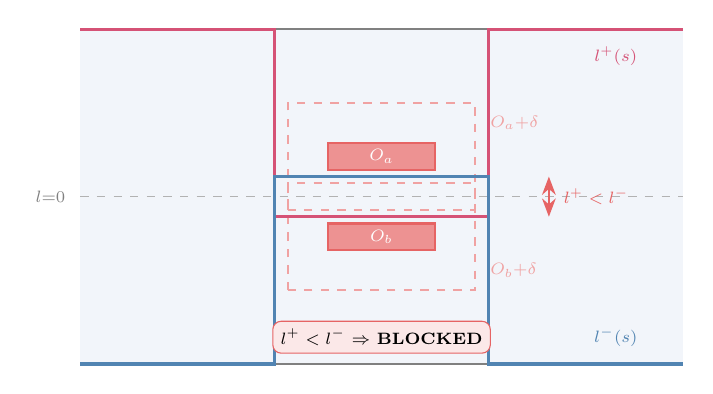
\begin{tikzpicture}[scale=0.85, transform shape]
  % 道路背景
  \fill[bglight] (-0.5,-2.5) rectangle (8.5,2.5);
  \draw[gray, thick] (-0.5, 2.5) -- (8.5, 2.5);
  \draw[gray, thick] (-0.5,-2.5) -- (8.5,-2.5);
  \draw[dashed, gray!60] (-0.5, 0) -- (8.5, 0);
  \node[gray, font=\scriptsize, anchor=east] at (-0.6, 0) {$l{=}0$};

  % O_a（上方）
  \fill[dangerred!70, draw=dangerred, thick] (3.2, 0.4) rectangle (4.8, 0.8);
  \node[font=\scriptsize, white] at (4.0, 0.6) {$O_a$};

  % O_b（下方）
  \fill[dangerred!70, draw=dangerred, thick] (3.2,-0.8) rectangle (4.8,-0.4);
  \node[font=\scriptsize, white] at (4.0,-0.6) {$O_b$};

  % 膨胀虚线 δ=0.6
  \draw[dangerred!60, dashed, thick] (2.6,-0.2) rectangle (5.4, 1.4);
  \node[dangerred!60, font=\scriptsize, anchor=west] at (5.5, 1.1) {$O_a{+}\delta$};
  \draw[dangerred!60, dashed, thick] (2.6,-1.4) rectangle (5.4, 0.2);
  \node[dangerred!60, font=\scriptsize, anchor=west] at (5.5,-1.1) {$O_b{+}\delta$};

  % 上界 l+(s)：右绕 O_a
  \draw[deeppink, very thick]
    (-0.5, 2.5) -- (2.4, 2.5) -- (2.4, -0.3) -- (5.6, -0.3) -- (5.6, 2.5) -- (8.5, 2.5);
  \node[deeppink, font=\scriptsize] at (7.5, 2.1) {$l^+(s)$};

  % 下界 l-(s)：左绕 O_b
  \draw[deepblue, very thick]
    (-0.5,-2.5) -- (2.4,-2.5) -- (2.4, 0.3) -- (5.6, 0.3) -- (5.6,-2.5) -- (8.5,-2.5);
  \node[deepblue, font=\scriptsize] at (7.5,-2.1) {$l^-(s)$};

  % 矛盾标注
  \draw[dangerred, thick, {Stealth}-{Stealth}] (6.5,-0.3) -- (6.5, 0.3);
  \node[dangerred, font=\scriptsize, anchor=west] at (6.6, 0) {$l^+ < l^-$};

  % BLOCKED 判定
  \node[draw=dangerred, fill=dangerred!15, font=\scriptsize,
        rounded corners=3pt, align=center] at (4.0,-2.1)
    {$l^+ < l^-$ $\Rightarrow$ \textbf{BLOCKED}};
\end{tikzpicture}
\end{center}\vspace*{\fill}\clearpage
\vspace*{\fill}\begin{center}% 子图(b)：全局协调，统一右绕 → 通行
\begin{tikzpicture}[scale=0.85, transform shape]
  % 道路背景
  \fill[bglight] (-0.5,-2.5) rectangle (8.5,2.5);
  \draw[gray, thick] (-0.5, 2.5) -- (8.5, 2.5);
  \draw[gray, thick] (-0.5,-2.5) -- (8.5,-2.5);
  \draw[dashed, gray!60] (-0.5, 0) -- (8.5, 0);
  \node[gray, font=\scriptsize, anchor=east] at (-0.6, 0) {$l{=}0$};

  % O_a（上方）
  \fill[dangerred!70, draw=dangerred, thick] (3.2, 0.4) rectangle (4.8, 0.8);
  \node[font=\scriptsize, white] at (4.0, 0.6) {$O_a$};

  % O_b（下方）
  \fill[dangerred!70, draw=dangerred, thick] (3.2,-0.8) rectangle (4.8,-0.4);
  \node[font=\scriptsize, white] at (4.0,-0.6) {$O_b$};

  % 膨胀虚线 δ=0.6
  \draw[dangerred!60, dashed, thick] (2.6,-0.2) rectangle (5.4, 1.4);
  \node[dangerred!60, font=\scriptsize, anchor=west] at (5.5, 0.6) {$O_a{+}\delta$};
  \draw[dangerred!60, dashed, thick] (2.6,-1.4) rectangle (5.4, 0.2);
  \node[dangerred!60, font=\scriptsize, anchor=west] at (5.5,-0.6) {$O_b{+}\delta$};

  % 上界 l+(s)：统一右绕，压到 O_b 膨胀下缘
  \draw[deeppink, very thick]
    (-0.5, 2.5) -- (2.4, 2.5) -- (2.4, -1.5) -- (5.6, -1.5) -- (5.6, 2.5) -- (8.5, 2.5);
  \node[deeppink, font=\scriptsize] at (7.5, 2.1) {$l^+(s)$};

  % 下界 l-(s)：道路下界
  \draw[deepblue, very thick, dashed]
    (-0.5,-2.5) -- (8.5,-2.5);
  \node[deepblue, font=\scriptsize, left] at (-0.6,-2.5) {$l^-(s)$};

  % 通行带
  \fill[lightgreen, opacity=0.25] (-0.5,-2.5) rectangle (8.5,-1.5);

  % 通行带宽度标注
  \draw[deeppink, thick, {Stealth}-{Stealth}] (0.5,-2.5) -- (0.5,-1.5);
  \node[deeppink, font=\scriptsize, anchor=east] at (0.4,-2.0) {$W{=}1.0$m};

  % 自车轨迹
  \draw[deepblue, very thick, -{Stealth}]
    plot[smooth, tension=0.55] coordinates
      {(0.5, 0) (1.5,-0.5) (2.5,-1.8) (4.0,-2.0) (5.5,-1.8) (6.5,-0.5) (7.5, 0)};
  \node[deepblue, font=\scriptsize] at (4.0,-2.45) {规划轨迹};

  % PASS 判定
  \node[draw=lightgreen!80!black, fill=lightgreen!20, font=\scriptsize,
        rounded corners=3pt, align=center] at (4.0, 2.0)
    {统一右绕 $\Rightarrow$ \textbf{PASS}};
\end{tikzpicture}
\end{center}\vspace*{\fill}\clearpage

% ============================================================
% 可行域压缩 子图a
% ============================================================
\vspace*{\fill}\begin{center}% 2 个障碍物 通行带可行（子图 a）
\begin{tikzpicture}[scale=0.7, transform shape]
  \draw[-Stealth, thick] (0,-2.5) -- (8.5,-2.5) node[right, font=\footnotesize] {$s$};
  \draw[-Stealth, thick] (0,-2.5) -- (0,2.5) node[above, font=\footnotesize] {$l$};

  \draw[gray, thick] (0,1.875) -- (8,1.875);
  \draw[gray, thick] (0,-1.875) -- (8,-1.875);
  \draw[gray, dashed] (0,0) -- (8,0);

  \begin{scope}[on background layer]
    \fill[bglight] (0,-1.875) rectangle (8,1.875);
  \end{scope}

  % O1（上方靠边）y=[0.6, 1.3], s=[2, 4]
  \fill[dangerred!70, draw=dangerred, thick] (2,0.6) rectangle (4,1.3);
  \node[white, font=\footnotesize\bfseries] at (3,0.95) {$O_1$};

  % O2（下方靠边）y=[-1.2, -0.5], s=[5, 7]
  \fill[dangerred!70, draw=dangerred, thick] (5,-1.2) rectangle (7,-0.5);
  \node[white, font=\footnotesize\bfseries] at (6,-0.85) {$O_2$};

  % O1 右绕 → 上界压到 O1 膨胀下缘 (0.6-0.4=0.2)
  \draw[deeppink, very thick]
    (0,1.875) -- (1.8,1.875) -- (1.8,0.2) -- (4.2,0.2) -- (4.2,1.875) -- (8,1.875);
  \node[deeppink, font=\tiny] at (1, 2.1) {$l^+(s)$};

  % O2 左绕 → 下界抬到 O2 膨胀上缘 (-0.5+0.4=-0.1)
  \draw[deepblue, very thick]
    (0,-1.875) -- (4.8,-1.875) -- (4.8,-0.1) -- (7.2,-0.1) -- (7.2,-1.875) -- (8,-1.875);
  \node[deepblue, font=\tiny] at (7.5, -2.1) {$l^-(s)$};

  \node[lightgreen!60!black, font=\footnotesize\bfseries] at (4,-1.35) {通行带充足};
\end{tikzpicture}
\end{center}\vspace*{\fill}\clearpage
% ============================================================
% 可行域压缩 子图b
% ============================================================
\vspace*{\fill}\begin{center}% 4 个障碍物 通行带狭窄（子图 b）
\begin{tikzpicture}[scale=0.7, transform shape]
  \draw[-Stealth, thick] (0,-2.5) -- (8.5,-2.5) node[right, font=\footnotesize] {$s$};
  \draw[-Stealth, thick] (0,-2.5) -- (0,2.5) node[above, font=\footnotesize] {$l$};

  \draw[gray, thick] (0,1.875) -- (8,1.875);
  \draw[gray, thick] (0,-1.875) -- (8,-1.875);
  \draw[gray, dashed] (0,0) -- (8,0);

  \begin{scope}[on background layer]
    \fill[bglight] (0,-1.875) rectangle (8,1.875);
  \end{scope}

  % O1（上方靠边）y=[0.5, 1.1], s=[1, 2.5]
  \fill[dangerred!70, draw=dangerred, thick] (1,0.5) rectangle (2.5,1.1);
  \node[white, font=\tiny\bfseries] at (1.75,0.8) {$O_1$};

  % O2（下方靠边）y=[-1.0, -0.4], s=[2.5, 4]
  \fill[dangerred!70, draw=dangerred, thick] (2.5,-1.0) rectangle (4,-0.4);
  \node[white, font=\tiny\bfseries] at (3.25,-0.7) {$O_2$};

  % O3（上方靠边）y=[0.4, 0.9], s=[4.5, 6]
  \fill[dangerred!70, draw=dangerred, thick] (4.5,0.4) rectangle (6,0.9);
  \node[white, font=\tiny\bfseries] at (5.25,0.65) {$O_3$};

  % O4（下方靠边）y=[-0.8, -0.2], s=[6, 7.5]
  \fill[dangerred!70, draw=dangerred, thick] (6,-0.8) rectangle (7.5,-0.2);
  \node[white, font=\tiny\bfseries] at (6.75,-0.5) {$O_4$};

  % 上界 l+(s)：O1右绕压到0.1, O3右绕压到0.0
  \draw[deeppink, very thick]
    (0,1.875) -- (0.8,1.875) -- (0.8,0.1) -- (2.7,0.1)
    -- (2.7,1.875) -- (4.3,1.875) -- (4.3,0.0) -- (6.2,0.0)
    -- (6.2,1.875) -- (8,1.875);

  % 下界 l-(s)：O2左绕抬到0.0, O4左绕抬到0.2
  \draw[deepblue, very thick]
    (0,-1.875) -- (2.3,-1.875) -- (2.3,0.0) -- (4.2,0.0)
    -- (4.2,-1.875) -- (5.8,-1.875) -- (5.8,0.2) -- (7.7,0.2)
    -- (7.7,-1.875) -- (8,-1.875);

  % 窄处标注
  \draw[lightorange, ultra thick] (2.5,0.0) -- (2.5,0.1);
  \node[lightorange!80!black, font=\tiny\bfseries, anchor=west] at (2.6,0.05) {窄};
  \draw[lightorange, ultra thick] (6,0.0) -- (6,0.2);
  \node[lightorange!80!black, font=\tiny\bfseries, anchor=west] at (6.1,0.1) {窄};

  \node[deeppink, font=\tiny] at (0.5, 2.1) {$l^+(s)$};
  \node[deepblue, font=\tiny] at (7.5, -2.1) {$l^-(s)$};
  \node[lightorange!80!black, font=\footnotesize\bfseries] at (4,-1.5) {多次收缩 通行带退化};
\end{tikzpicture}
\end{center}\vspace*{\fill}\clearpage
% ============================================================
% 可行域压缩 子图c
% ============================================================
\vspace*{\fill}\begin{center}% 密集障碍物 BLOCKED（子图 c）
\begin{tikzpicture}[scale=0.7, transform shape]
  \draw[-Stealth, thick] (0,-2.5) -- (8.5,-2.5) node[right, font=\footnotesize] {$s$};
  \draw[-Stealth, thick] (0,-2.5) -- (0,2.5) node[above, font=\footnotesize] {$l$};

  \draw[gray, thick] (0,1.875) -- (8,1.875);
  \draw[gray, thick] (0,-1.875) -- (8,-1.875);
  \draw[gray, dashed] (0,0) -- (8,0);

  \begin{scope}[on background layer]
    \fill[bglight] (0,-1.875) rectangle (8,1.875);
  \end{scope}

  % 密集障碍物（交替上下，靠近道路边缘）
  \fill[dangerred!70, draw=dangerred, thick] (0.5,0.4) rectangle (1.5,1.2);
  \node[white, font=\tiny\bfseries] at (1,0.8) {$O_1$};

  \fill[dangerred!70, draw=dangerred, thick] (1.5,-1.1) rectangle (2.5,-0.3);
  \node[white, font=\tiny\bfseries] at (2,-0.7) {$O_2$};

  \fill[dangerred!70, draw=dangerred, thick] (2.5,0.3) rectangle (3.5,1.1);
  \node[white, font=\tiny\bfseries] at (3,0.7) {$O_3$};

  \fill[dangerred!70, draw=dangerred, thick] (3.5,-1.0) rectangle (4.5,-0.2);
  \node[white, font=\tiny\bfseries] at (4,-0.6) {$O_4$};

  \fill[dangerred!70, draw=dangerred, thick] (4.5,0.5) rectangle (5.5,1.3);
  \node[white, font=\tiny\bfseries] at (5,0.9) {$O_5$};

  \fill[dangerred!70, draw=dangerred, thick] (5.5,-1.2) rectangle (6.5,-0.3);
  \node[white, font=\tiny\bfseries] at (6,-0.75) {$O_6$};

  \fill[dangerred!70, draw=dangerred, thick] (6.5,0.3) rectangle (7.5,1.1);
  \node[white, font=\tiny\bfseries] at (7,0.7) {$O_7$};

  % 上界 l+(s)：逐步压低 (δ=0.4)
  \draw[deeppink, very thick]
    (0,1.875) -- (0.3,1.875) -- (0.3,0.0) -- (1.7,0.0)
    -- (1.7,1.875) -- (2.3,1.875) -- (2.3,-0.1) -- (3.7,-0.1)
    -- (3.7,1.875) -- (4.3,1.875) -- (4.3,0.1) -- (5.7,0.1);

  % 下界 l-(s)：逐步抬高
  \draw[deepblue, very thick]
    (0,-1.875) -- (1.3,-1.875) -- (1.3,0.1) -- (2.7,0.1)
    -- (2.7,-1.875) -- (3.3,-1.875) -- (3.3,0.2) -- (4.7,0.2);

  % BLOCKED 点
  \fill[dangerred] (4.5,0.15) circle (3pt);

  % 截断区域
  \fill[dangerred, opacity=0.1] (4.5,-1.875) rectangle (8,1.875);
  \node[dangerred, font=\footnotesize\bfseries] at (6.5,1.3) {$l^+ < l^- \rightarrow$ BLOCKED};
  \node[dangerred, font=\tiny] at (6.5,-1.5) {TrimPathBounds 截断};

  \node[deeppink, font=\tiny] at (0.5, 2.1) {$l^+(s)$};
  \node[deepblue, font=\tiny] at (0.5, -2.1) {$l^-(s)$};
\end{tikzpicture}
\end{center}\vspace*{\fill}\clearpage

% ============================================================
% ST边界累积膨胀
% ============================================================

\vspace*{\fill}
\begin{center}
% ST边界累积膨胀示意图
\begin{tikzpicture}[scale=0.75, transform shape]
  % ===== 左图：独立扩展 =====
  \node[font=\small\bfseries] at (4, 7.5) {(a) 独立扩展（Apollo原始）};

  % 坐标轴
  \draw[-Stealth, thick] (0,0) -- (8.5,0) node[right, font=\footnotesize] {$t$};
  \draw[-Stealth, thick] (0,0) -- (0,7) node[above, font=\footnotesize] {$s$};

  % 障碍物1（实际）
  \fill[dangerred!40] (0,1.5) rectangle (7.5,2.5);
  \node[font=\tiny, dangerred] at (1.2, 2.0) {Obs 1};

  % 障碍物1 扩展区域
  \fill[dangerred!15] (0,0.5) rectangle (7.5,1.5);
  \fill[dangerred!15] (0,2.5) rectangle (7.5,3.5);

  % 障碍物2（实际）
  \fill[lightorange!60] (0,3.8) rectangle (7.5,4.8);
  \node[font=\tiny, lightorange!80!black] at (1.2, 4.3) {Obs 2};

  % 障碍物2 扩展区域
  \fill[lightorange!30] (0,2.8) rectangle (7.5,3.8);
  \fill[lightorange!30] (0,4.8) rectangle (7.5,5.8);

  % 障碍物3（实际）
  \fill[deepblue!40] (0,6.0) rectangle (7.5,6.5);
  \node[font=\tiny, deepblue] at (1.2, 6.25) {Obs 3};

  % 障碍物3 扩展区域
  \fill[deepblue!15] (0,5.0) rectangle (7.5,6.0);

  % 重叠区域标注
  \draw[very thick, deeppink, <->] (8.0, 2.5) -- (8.0, 3.5);
  \node[deeppink, font=\tiny, right] at (8.0, 3.0) {重叠};

  \draw[very thick, deeppink, <->] (8.0, 4.8) -- (8.0, 5.8);
  \node[deeppink, font=\tiny, right] at (8.0, 5.3) {重叠};

  % 扩展距离标注
  \draw[{Stealth}-{Stealth}, thick, gray] (-0.6, 1.5) -- (-0.6, 0.5);
  \node[gray, font=\tiny, left] at (-0.6, 1.0) {$d_{ext}$};

  % ===== 右图：合并后 =====
  \begin{scope}[xshift=11cm]
    \node[font=\small\bfseries] at (4, 7.5) {(b) 合并后（改进方案）};

    \draw[-Stealth, thick] (0,0) -- (8.5,0) node[right, font=\footnotesize] {$t$};
    \draw[-Stealth, thick] (0,0) -- (0,7) node[above, font=\footnotesize] {$s$};

    % 合并后的整体边界
    \fill[dangerred!25] (0,0.5) rectangle (7.5,6.5);

    % 实际障碍物
    \fill[dangerred!50] (0,1.5) rectangle (7.5,2.5);
    \fill[lightorange!70] (0,3.8) rectangle (7.5,4.8);
    \fill[deepblue!50] (0,6.0) rectangle (7.5,6.5);

    % 只在整体边界外扩展一次
    \draw[very thick, lightgreen!70!black, dashed] (0,0.5) -- (7.5,0.5);
    \draw[very thick, lightgreen!70!black, dashed] (0,6.5) -- (7.5,6.5);

    % 标注
    \draw[{Stealth}-{Stealth}, thick, lightgreen!70!black] (-0.6, 0.5) -- (-0.6, 6.5);
    \node[lightgreen!70!black, font=\tiny, left, align=center] at (-0.6, 3.5) {合并区域\\仅外扩一次};

    % 可行域标注
    \fill[lightgreen!20] (0,0) rectangle (7.5,0.5);
    \node[lightgreen!70!black, font=\tiny] at (3.8, 0.25) {可行域};
  \end{scope}

  % 箭头连接
  \draw[-Stealth, ultra thick, deeppink] (9, 3.5) -- (10.5, 3.5) node[midway, above, font=\footnotesize\bfseries] {合并};
\end{tikzpicture}

\end{center}
\vspace*{\fill}

\clearpage

% ============================================================
% 威胁度雷达图 子图a
% ============================================================
\vspace*{\fill}\begin{center}% 高威胁障碍物雷达图（子图 a）
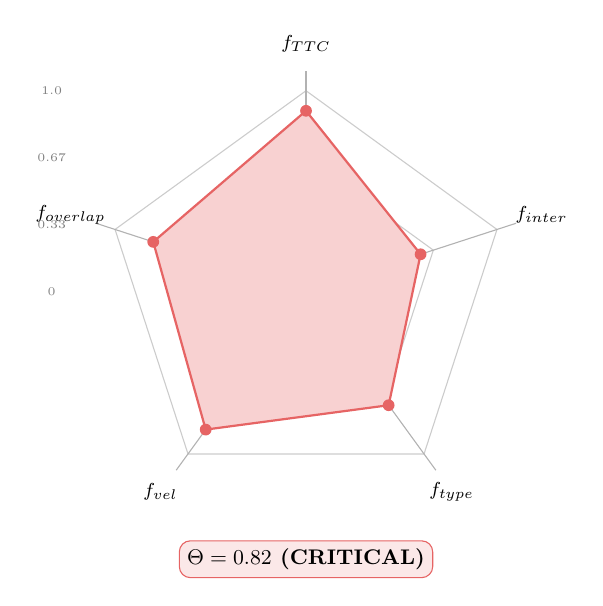
\begin{tikzpicture}[scale=0.85, transform shape]
  \foreach \r in {1, 2, 3} {
    \draw[gray!40, thin] (90:\r) \foreach \a in {162, 234, 306, 378} { -- (\a:\r) } -- cycle;
  }
  \foreach \a/\lbl in {90/$f_{TTC}$, 162/$f_{overlap}$, 234/$f_{vel}$, 306/$f_{type}$, 378/$f_{inter}$} {
    \draw[gray!60, thin] (0,0) -- (\a:3.3);
    \node[font=\footnotesize] at (\a:3.7) {\lbl};
  }

  \fill[dangerred!30, draw=dangerred, thick]
    (90:2.7) -- (162:2.4) -- (234:2.55) -- (306:2.1) -- (378:1.8) -- cycle;
  \foreach \a/\r in {90/2.7, 162/2.4, 234/2.55, 306/2.1, 378/1.8} {
    \fill[dangerred] (\a:\r) circle (2.5pt);
  }

  \node[draw=dangerred, fill=dangerred!15, rounded corners, font=\small\bfseries] at (0, -4) {$\Theta = 0.82$ (CRITICAL)};

  \node[gray, font=\tiny] at (-3.8, 0) {0};
  \node[gray, font=\tiny] at (-3.8, 1.0) {0.33};
  \node[gray, font=\tiny] at (-3.8, 2.0) {0.67};
  \node[gray, font=\tiny] at (-3.8, 3.0) {1.0};
\end{tikzpicture}
\end{center}\vspace*{\fill}\clearpage
% ============================================================
% 威胁度雷达图 子图b
% ============================================================
\vspace*{\fill}\begin{center}% 低威胁障碍物雷达图（子图 b）
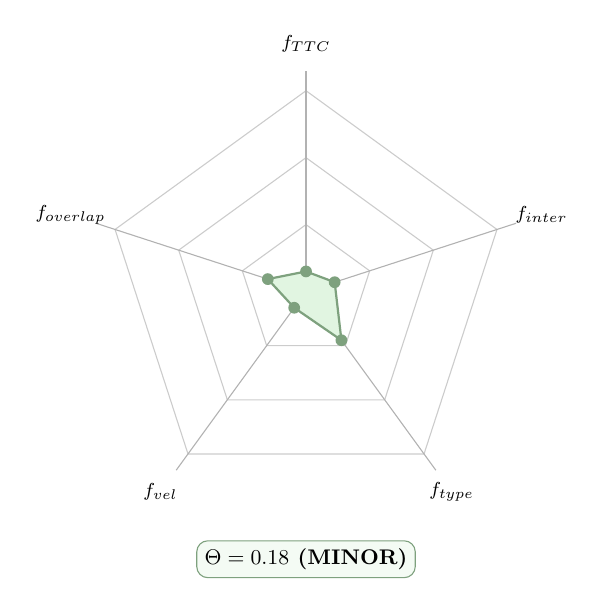
\begin{tikzpicture}[scale=0.85, transform shape]
  \foreach \r in {1, 2, 3} {
    \draw[gray!40, thin] (90:\r) \foreach \a in {162, 234, 306, 378} { -- (\a:\r) } -- cycle;
  }
  \foreach \a/\lbl in {90/$f_{TTC}$, 162/$f_{overlap}$, 234/$f_{vel}$, 306/$f_{type}$, 378/$f_{inter}$} {
    \draw[gray!60, thin] (0,0) -- (\a:3.3);
    \node[font=\footnotesize] at (\a:3.7) {\lbl};
  }

  \fill[lightgreen!40, draw=lightgreen!70!black, thick]
    (90:0.3) -- (162:0.6) -- (234:0.3) -- (306:0.9) -- (378:0.45) -- cycle;
  \foreach \a/\r in {90/0.3, 162/0.6, 234/0.3, 306/0.9, 378/0.45} {
    \fill[lightgreen!70!black] (\a:\r) circle (2.5pt);
  }

  \node[draw=lightgreen!70!black, fill=lightgreen!15, rounded corners, font=\small\bfseries] at (0, -4) {$\Theta = 0.18$ (MINOR)};
\end{tikzpicture}
\end{center}\vspace*{\fill}\clearpage

% ============================================================
% 时空走廊生成过程
% ============================================================

\vspace*{\fill}\begin{center}% 子图(a)：s=s^* 处的横向切片，按式 \eqref{eq:time_varying_gap} 分析 l 方向间隙
% 场景参数：W_ego=1.5；A 在 s^*=3.25 处的 l 投影 [u_A,v_A]=[-1.2,0.3]
\begin{tikzpicture}[scale=1.0, transform shape]
  % 统一 bounding box，与 b、c 图宽高比对齐 (宽:高 ≈ 1.25:1)
  \useasboundingbox (-3.2, -2.3) rectangle (3.2, 2.9);

  % 道路底色放到 background layer，避免覆盖 l 轴刻度与障碍物
  \begin{scope}[on background layer]
    \fill[bglight] (-2, -0.6) rectangle (2, 0.6);
  \end{scope}

  % l 轴
  \draw[-Stealth, thick] (-2.6, 0) -- (2.8, 0) node[right, font=\footnotesize] {$l$};
  \foreach \x in {-2, -1, 0, 1, 2} {
    \draw[thin] (\x, -0.08) -- (\x, 0.08);
    \node[font=\tiny, below=2pt] at (\x, -0.08) {$\x$};
  }

  % 道路上下边界
  \draw[gray!70, thick] (-2, 0.6) -- (2, 0.6);
  \draw[gray!70, thick] (-2, -0.6) -- (2, -0.6);
  \node[gray, font=\tiny, above] at (-2, 0.62) {$l_{road}^{-}$};
  \node[gray, font=\tiny, above] at (2, 0.62) {$l_{road}^{+}$};

  % 障碍物 A 的 l 投影 [u_A, v_A] = [-1.2, 0.3]
  \fill[dangerred!35, draw=dangerred, thick] (-1.2, -0.5) rectangle (0.3, 0.5);
  \node[font=\scriptsize\bfseries, white] at (-0.45, 0) {A};
  \draw[dangerred, thick] (-1.2, -0.5) -- (-1.2, -1.0);
  \draw[dangerred, thick] (0.3, -0.5) -- (0.3, -1.0);
  \node[dangerred, font=\tiny] at (-1.2, -1.22) {$u_A{=}-1.2$};
  \node[dangerred, font=\tiny] at (0.3, -1.22) {$v_A{=}0.3$};

  % 间隙 g_0 = u_A - l_road^- = 0.8；g_1 = l_road^+ - v_A = 1.7
  \draw[lightgreen!70!black, very thick, |-|] (-2, 1.15) -- (-1.2, 1.15);
  \node[lightgreen!70!black, font=\scriptsize] at (-1.6, 1.42) {$g_0{=}0.8$};

  \draw[lightgreen!70!black, very thick, |-|] (0.3, 1.15) -- (2, 1.15);
  \node[lightgreen!70!black, font=\scriptsize] at (1.15, 1.42) {$g_1{=}1.7$};

  % W_ego 参考标尺（居中放在上方，长度严格 1.5）
  \draw[deepblue, very thick, |-|] (-0.75, 1.93) -- (0.75, 1.93);
  \node[deepblue, font=\scriptsize] at (0, 2.20) {$W_{ego}{=}1.5$};

  % 判定结果
  \node[dangerred, font=\scriptsize\bfseries] at (-1.6, 0.88) {$\times$};
  \node[lightgreen!50!black, font=\scriptsize\bfseries] at (1.15, 0.88) {$\checkmark$};

  % 自车（宽度 1.5）正好嵌在 g_1 中
  \fill[deepblue!45, draw=deepblue, thick] (0.35, -0.4) rectangle (1.85, 0.4);
  \node[deepblue, font=\tiny] at (1.1, 0) {自车};

  % 标题
  \node[font=\footnotesize\bfseries] at (0, 2.72) {$s{=}s^\star$ 横向切片};
  \node[font=\tiny, gray!70!black] at (0, -1.90) {在 $t{=}\tau(s^\star)$ 评估，$p^*{=}1$};
\end{tikzpicture}
\end{center}\vspace*{\fill}\clearpage
\vspace*{\fill}\begin{center}% 子图 (b)：g_{p^*}(s) 沿全 s 的剖面，与 W_ego 比较
% A 静态偏置 s in [2.5, 4], l in [-1.2, 0.3]: g_{p^*} = g_1 = 1.7, ok
% D 动态宽体 s ∈ [6.5, 7]，t=0 时 l ∈ [-1.3, 1.3]，v_lat = +0.4 m/s
%   τ(s) = s/4 → D 中心 +0.4·τ(s) = +0.1·s，D(τ) ⇒ l ∈ [-1.3 + 0.1s, 1.3 + 0.1s]
%   两侧间隙：左 g_0(s) = (-1.3 + 0.1s) + 2 = 0.7 + 0.1s ∈ [1.35, 1.40]
%             右 g_1(s) =  2 - (1.3 + 0.1s)   = 0.7 - 0.1s ∈ [0.30, 0.35]
%   max-gap p^* = 0（左），g_{p^*}(s) = 0.7 + 0.1s 在 s∈[6.5, 7] 从 1.35 微升到 1.40
%   全段 < W_ego = 1.5 → 禁行切片
\begin{tikzpicture}
\begin{axis}[
    width=8.4cm, height=6.0cm,
    xlabel={$s$ (m)}, ylabel={$g_{p^\star}(s)$ (m)},
    xmin=0, xmax=9, ymin=0, ymax=4.4,
    grid=major, grid style={gray!18},
    axis line style={thick},
    tick label style={font=\footnotesize},
    label style={font=\small\bfseries},
    legend style={
        font=\scriptsize,
        legend columns=-1,
        column sep=1.0em,
        at={(0.5, -0.25)}, anchor=north,
        draw=none, fill=none,
    },
    legend cell align=left,
    legend image post style={line width=1.0pt},
]

% ===== 禁行切片背景（D 段，s ∈ [6.5, 7]，全列填红）=====
\fill[dangerred!15] (axis cs:6.5, 0) rectangle (axis cs:7, 4.4);

% ===== s^* = 3.25 引线，呼应 (a) =====
\draw[gray!55!black, thin, dashed] (axis cs:3.25, 0) -- (axis cs:3.25, 1.7);
\filldraw[deepblue] (axis cs:3.25, 1.7) circle (1.6pt);
\node[deepblue!75!black, font=\scriptsize, anchor=south] at (axis cs:3.25, 1.78) {$s^\star$};

% ===== 主曲线 g_{p^*}(s) =====
\addplot[deepblue, very thick] coordinates {
    (0,    4)
    (2.5,  4)
    (2.5,  1.7)
    (4,    1.7)
    (4,    4)
    (6.5,  4)
    (6.5,  1.35)
    (7,    1.40)
    (7,    4)
    (9,    4)
};
\addlegendentry{$g_{p^\star}(s)$}

% ===== W_ego 参考虚线 =====
\addplot[dangerred, very thick, densely dashed] coordinates {(0, 1.5) (9, 1.5)};
\addlegendentry{$W_{ego} = 1.5$}

% ===== A 段标记（s ∈ [2.5, 4]） =====
\draw[dangerred, thick] (axis cs:2.5, 0.18) -- (axis cs:4, 0.18);
\node[dangerred, font=\scriptsize] at (axis cs:3.25, 0.50) {A 静态};

% ===== D 段标记（s ∈ [6.5, 7]） =====
\draw[dangerred, thick] (axis cs:6.5, 0.18) -- (axis cs:7, 0.18);
\node[dangerred, font=\scriptsize] at (axis cs:6.75, 0.50) {D 动态};

% ===== 判定标注 =====
\node[lightgreen!40!black, font=\scriptsize] at (axis cs:3.25, 2.10) {$\geq W_{ego}$ $\checkmark$};
\node[dangerred, font=\scriptsize] at (axis cs:7.55, 1.05) {$<W_{ego}$ $\times$};

% ===== 静态/动态对照（小字解释）=====
\node[deepblue!65!black, font=\tiny, align=center] at (axis cs:3.25, 1.05) {剖面平直};
\node[deepblue!65!black, font=\tiny, align=center] at (axis cs:6.75, 1.05) {随 $\tau$ 走};

% ===== 禁行切片标注 =====
\node[dangerred, font=\scriptsize, align=center]
    at (axis cs:6.75, 3.70) {禁行切片\\($\tau$ 引致)};

\end{axis}
\end{tikzpicture}
\end{center}\vspace*{\fill}\clearpage
\vspace*{\fill}\begin{center}% 子图 (c)：将通行 s 区间投至 ST 平面 ∩ 可达集 {t ≥ τ(s)}，得到走廊 Ω
% τ(s) = s/4 ⇒ ST 图上为过 (0,0) 与 (2.25, 9) 的直线
% 通行段：s ∈ [0, 6.5] ∪ [7, 9]；禁行切片：s ∈ [6.5, 7]
% Ω 下半段：(0,0) (1.625, 6.5) (3, 6.5) (3, 0)
% Ω 上半段：(1.75, 7) (2.25, 9) (3, 9) (3, 7)
% QP 轨迹严格起自 (0, 0)，紧贴 τ(s) 右下，止于禁行切片下沿 s ≈ 6.45
\begin{tikzpicture}
\begin{axis}[
    width=8.4cm, height=6.4cm,
    xlabel={$t$ (s)}, ylabel={$s$ (m)},
    xmin=0, xmax=3, ymin=0, ymax=9,
    grid=major, grid style={gray!18},
    axis line style={thick},
    tick label style={font=\footnotesize},
    label style={font=\small\bfseries},
    legend style={
        font=\scriptsize,
        legend columns=-1,
        column sep=0.9em,
        at={(0.5, -0.22)}, anchor=north,
        draw=none, fill=none,
    },
    legend cell align=left,
    legend image post style={line width=1.0pt},
]

% ===== 不可达区 t < τ(s)：(0,0) (2.25, 9) (0, 9) 三角 =====
\fill[gray!18]
    (axis cs:0, 0) -- (axis cs:2.25, 9) -- (axis cs:0, 9) -- cycle;

% ===== Ω 走廊 下半段 s ∈ [0, 6.5] =====
\fill[lightgreen!35]
    (axis cs:0, 0) -- (axis cs:1.625, 6.5)
    -- (axis cs:3, 6.5) -- (axis cs:3, 0) -- cycle;

% ===== Ω 走廊 上半段 s ∈ [7, 9] =====
\fill[lightgreen!35]
    (axis cs:1.75, 7) -- (axis cs:2.25, 9)
    -- (axis cs:3, 9) -- (axis cs:3, 7) -- cycle;

% ===== 禁行切片 s ∈ [6.5, 7] × 全 t =====
\fill[dangerred!25] (axis cs:0, 6.5) rectangle (axis cs:3, 7);
\draw[dangerred, thick, dashed] (axis cs:0, 6.5) -- (axis cs:3, 6.5);
\draw[dangerred, thick, dashed] (axis cs:0, 7  ) -- (axis cs:3, 7  );

% ===== τ(s) = s/4 蓝色虚线 =====
\addplot[deepblue, very thick, densely dashed] coordinates {(0, 0) (2.25, 9)};
\addlegendentry{$\tau(s) = s/4$}

% ===== Ω 走廊（图例占位用色块）=====
\addplot[lightgreen!35, fill=lightgreen!35, mark=none, forget plot] coordinates {(-1, -1)};
\addlegendimage{area legend, fill=lightgreen!35, draw=lightgreen!50!black}
\addlegendentry{$\Omega$ 走廊}

% ===== 禁行切片图例占位 =====
\addlegendimage{area legend, fill=dangerred!25, draw=dangerred}
\addlegendentry{禁行切片}

% ===== QP 最优轨迹 s(t) =====
\addplot[deeppink, very thick, -{Stealth}] coordinates {
    (0,    0)
    (0.15, 0.5)
    (0.32, 1.2)
    (0.55, 2.1)
    (0.80, 3.1)
    (1.05, 4.1)
    (1.30, 5.1)
    (1.55, 6.1)
    (1.70, 6.45)
};
\addlegendentry{QP 轨迹 $s(t)$}

% ===== 文字标注 =====
\node[lightgreen!35!black, font=\footnotesize\bfseries] at (axis cs:2.45, 3.0) {$\Omega$};
\node[dangerred!85!black, font=\tiny, anchor=west]
    at (axis cs:0.05, 8.55) {D 在 $t = \tau$ 时仍堵塞};
\node[dangerred, font=\scriptsize] at (axis cs:2.50, 6.75) {禁行切片};
\node[gray!55!black, font=\scriptsize, align=center]
    at (axis cs:0.55, 7.55) {$t < \tau(s)$\\不可达};

% ===== s 轴侧标 A、D 区间 =====
\draw[dangerred, thick] (axis cs:-0.04, 2.5) -- (axis cs:-0.04, 4);
\node[dangerred, font=\tiny, anchor=east] at (axis cs:-0.06, 3.25) {A};
\draw[dangerred, thick] (axis cs:-0.04, 6.5) -- (axis cs:-0.04, 7);
\node[dangerred, font=\tiny, anchor=east] at (axis cs:-0.06, 6.75) {D};

\end{axis}
\end{tikzpicture}
\end{center}\vspace*{\fill}\clearpage

% ============================================================
% 约束转化对比 子图a
% ============================================================
\vspace*{\fill}\begin{center}% Apollo原始多独立ST约束（子图 a）
\begin{tikzpicture}[scale=0.75, transform shape]
  \draw[-Stealth, thick] (0,0) -- (8.5,0) node[right, font=\footnotesize] {$t$};
  \draw[-Stealth, thick] (0,0) -- (0,7.5) node[above, font=\footnotesize] {$s$};

  % 三个独立 ST boundary 禁行区
  \fill[dangerred!30, draw=dangerred, thick] (0,1.0) rectangle (7.5,2.0);
  \fill[lightorange!30, draw=lightorange!80!black, thick] (1,3.5) -- (6,4.5) -- (6,5.2) -- (1,4.2) -- cycle;
  \fill[deepblue!20, draw=deepblue, thick] (2,5.8) rectangle (7.5,6.6);

  \node[dangerred, font=\footnotesize] at (-0.8, 1.5) {$B_1$};
  \node[lightorange!80!black, font=\footnotesize] at (-0.8, 3.8) {$B_2$};
  \node[deepblue, font=\footnotesize] at (-0.8, 6.2) {$B_3$};

  % 每个 boundary 的 YIELD/OVERTAKE 离散选择标注
  \node[dangerred, font=\tiny, align=center] at (3.75, 1.5) {YIELD 或 OVERTAKE?};
  \node[lightorange!80!black, font=\tiny, align=center] at (3.5, 4.85) {YIELD 或 OVERTAKE?};
  \node[deepblue, font=\tiny, align=center] at (4.75, 6.2) {YIELD 或 OVERTAKE?};

  % 底部标注
  \node[draw=dangerred, fill=dangerred!10, rounded corners, font=\footnotesize, align=center] at (4, -1.2) {$2^n$ 种 YIELD/OVERTAKE 组合\\非凸离散选择 \;\; DP 启发式搜索};

  % DP搜索路径（锯齿穿行）
  \draw[thick, deepblue, dashed, -{Stealth}]
    plot[smooth, tension=0.4] coordinates {(0,0.3) (1,0.8) (2,2.5) (3,3.0) (4,3.2) (5,5.5) (6,5.6) (7,5.7)};
  \node[deepblue, font=\tiny\bfseries] at (6.5, 5.2) {DP路径};
\end{tikzpicture}
\end{center}\vspace*{\fill}\clearpage
% ============================================================
% 约束转化对比 子图b
% ============================================================
\vspace*{\fill}\begin{center}% 改进方案走廊约束（子图 b）
\begin{tikzpicture}[scale=0.75, transform shape]
  \draw[-Stealth, thick] (0,0) -- (8.5,0) node[right, font=\footnotesize] {$t$};
  \draw[-Stealth, thick] (0,0) -- (0,7.5) node[above, font=\footnotesize] {$s$};

  \fill[gray!15] (0,1.0) rectangle (7.5,2.0);
  \fill[gray!15] (1,3.5) -- (6,4.5) -- (6,5.2) -- (1,4.2) -- cycle;
  \fill[gray!15] (2,5.8) rectangle (7.5,6.6);

  \fill[lightgreen!30]
    plot[smooth] coordinates {(0,0.2) (1,0.3) (2,0.4) (3,2.2) (4,2.3) (5,2.4) (6,2.5) (7,2.6)}
    -- plot[smooth] coordinates {(7,3.3) (6,3.2) (5,3.1) (4,3.0) (3,2.9) (2,0.9) (1,0.8) (0,0.7)}
    -- cycle;
  \draw[very thick, lightgreen!70!black]
    plot[smooth] coordinates {(0,0.2) (1,0.3) (2,0.4) (3,2.2) (4,2.3) (5,2.4) (6,2.5) (7,2.6)};
  \draw[very thick, lightgreen!70!black]
    plot[smooth] coordinates {(0,0.7) (1,0.8) (2,0.9) (3,2.9) (4,3.0) (5,3.1) (6,3.2) (7,3.3)};

  \node[lightgreen!70!black, font=\footnotesize\bfseries] at (5.5, 1.8) {走廊 $\Omega$};

  \draw[{Stealth}-{Stealth}, thick, lightgreen!70!black] (7.8, 2.6) -- (7.8, 3.3);
  \node[lightgreen!70!black, font=\tiny, right] at (7.9, 2.95) {$s_{lower}^{\Omega} \leq s \leq s_{upper}^{\Omega}$};

  \draw[very thick, deepblue, -{Stealth}]
    plot[smooth] coordinates {(0,0.5) (1,0.6) (2,0.7) (3,2.6) (4,2.7) (5,2.8) (6,2.9) (7,3.0)};
  \node[deepblue, font=\footnotesize\bfseries] at (5, 3.6) {QP全局最优};

  \node[draw=lightgreen!70!black, fill=lightgreen!10, rounded corners, font=\footnotesize, align=center] at (4, -1) {约束 $s_{lower}^{\Omega}(t_k) \leq s_k \leq s_{upper}^{\Omega}(t_k)$\\凸 \;\; 约束数 $O(K)$};
\end{tikzpicture}
\end{center}\vspace*{\fill}\clearpage

% ============================================================
% 四类测试场景
% ============================================================

\vspace*{\fill}
\begin{center}
% 四类测试场景布局示意图
\begin{tikzpicture}[scale=0.55, transform shape]
  % ===== 场景一：纵向密集静态 =====
  \node[font=\small\bfseries] at (4, 4.5) {场景一：纵向密集静态障碍物};

  % 道路
  \fill[bglight] (0, -1.5) rectangle (8, 1.5);
  \draw[thick, gray] (0,1.5) -- (8,1.5);
  \draw[thick, gray] (0,-1.5) -- (8,-1.5);
  \draw[dashed, gray] (0,0) -- (8,0);

  % 自车
  \fill[deepblue, rounded corners=1pt] (0.3,-0.35) rectangle (1.2,0.35);
  \node[white, font=\tiny] at (0.75,0) {E};

  % 纵向排列的障碍物
  \foreach \x in {2.5, 4.0, 5.5, 7.0} {
    \fill[dangerred!60, rounded corners=1pt] (\x,-0.3) rectangle (\x+0.8,0.3);
  }
  \draw[{Stealth}-{Stealth}, thin, deeppink] (3.3, -0.7) -- (4.0, -0.7);
  \node[deeppink, font=\tiny] at (3.65, -1.1) {间距};

  % ===== 场景二：横向密集 =====
  \begin{scope}[xshift=10cm]
    \node[font=\small\bfseries] at (4, 4.5) {场景二：横向密集障碍物};

    \fill[bglight] (0, -2.5) rectangle (8, 2.5);
    \draw[thick, gray] (0,2.5) -- (8,2.5);
    \draw[thick, gray] (0,-2.5) -- (8,-2.5);
    \draw[dashed, gray] (0,0) -- (8,0);

    % 自车
    \fill[deepblue, rounded corners=1pt] (0.3,-0.35) rectangle (1.2,0.35);
    \node[white, font=\tiny] at (0.75,0) {E};

    % 上方障碍物
    \fill[dangerred!60, rounded corners=1pt] (3, 0.8) rectangle (5.5, 2.0);
    % 下方障碍物
    \fill[lightorange!70, rounded corners=1pt] (3.5, -2.0) rectangle (6, -0.8);

    % 窄通道
    \fill[lightgreen!20] (3, -0.8) rectangle (6, 0.8);
    \draw[{Stealth}-{Stealth}, thin, lightgreen!70!black] (6.3, -0.8) -- (6.3, 0.8);
    \node[lightgreen!70!black, font=\tiny, right] at (6.4, 0) {窄通道};
  \end{scope}

  % ===== 场景三：混合动静态 =====
  \begin{scope}[yshift=-7cm]
    \node[font=\small\bfseries] at (4, 4.5) {场景三：混合动静态障碍物};

    \fill[bglight] (0, -1.5) rectangle (8, 1.5);
    \draw[thick, gray] (0,1.5) -- (8,1.5);
    \draw[thick, gray] (0,-1.5) -- (8,-1.5);
    \draw[dashed, gray] (0,0) -- (8,0);

    % 自车
    \fill[deepblue, rounded corners=1pt] (0.3,-0.35) rectangle (1.2,0.35);
    \node[white, font=\tiny] at (0.75,0) {E};

    % 静态障碍物
    \fill[dangerred!60, rounded corners=1pt] (3, 0.6) rectangle (3.8, 1.2);
    \node[font=\tiny] at (3.4, 0.3) {静态};

    % 动态障碍物（带速度箭头）
    \fill[lightorange!70, rounded corners=1pt] (5, -0.3) rectangle (5.8, 0.3);
    \draw[-Stealth, thick, lightorange!80!black] (5.8, 0) -- (6.5, 0);
    \node[font=\tiny] at (6.2, -0.4) {动态};

    % 行人
    \fill[deeppink] (6.5, 1.0) circle (4pt);
    \draw[-Stealth, thin, deeppink] (6.5, 1.0) -- (6.5, 0.3);
    \node[font=\tiny, deeppink] at (7.2, 1.0) {行人};
  \end{scope}

  % ===== 场景四：交叉路口 =====
  \begin{scope}[xshift=10cm, yshift=-7cm]
    \node[font=\small\bfseries] at (4, 4.5) {场景四：高密度交叉路口};

    % 交叉路口
    \fill[bglight] (0, -0.5) rectangle (8, 3.5);
    \fill[bglight] (2.5, -2.5) rectangle (5.5, 4.5);
    \draw[thick, gray] (0, 3.5) -- (2.5, 3.5);
    \draw[thick, gray] (5.5, 3.5) -- (8, 3.5);
    \draw[thick, gray] (0, -0.5) -- (2.5, -0.5);
    \draw[thick, gray] (5.5, -0.5) -- (8, -0.5);
    \draw[thick, gray] (2.5, 4.5) -- (2.5, 3.5);
    \draw[thick, gray] (5.5, 4.5) -- (5.5, 3.5);
    \draw[thick, gray] (2.5, -2.5) -- (2.5, -0.5);
    \draw[thick, gray] (5.5, -2.5) -- (5.5, -0.5);

    % 自车（从左进入）
    \fill[deepblue, rounded corners=1pt] (0.5, 1.2) rectangle (1.5, 1.8);
    \draw[-Stealth, thick, deepblue] (1.5, 1.5) -- (2.3, 1.5);

    % 多方向来车
    \fill[dangerred!60, rounded corners=1pt] (6, 1.7) rectangle (7, 2.3);
    \draw[-Stealth, thick, dangerred] (6, 2.0) -- (5.3, 2.0);

    \fill[lightorange!70, rounded corners=1pt] (3.7, 4.0) rectangle (4.3, 3.2);
    \draw[-Stealth, thick, lightorange!80!black] (4.0, 3.2) -- (4.0, 2.5);

    \fill[lightgreen!60!black, rounded corners=1pt] (3.2, -2.0) rectangle (3.8, -1.2);
    \draw[-Stealth, thick, lightgreen!60!black] (3.5, -1.2) -- (3.5, -0.3);

    % 行人
    \fill[deeppink] (4.5, 0.5) circle (3pt);
    \fill[deeppink] (3.0, 2.8) circle (3pt);
    \draw[-Stealth, thin, deeppink] (4.5, 0.5) -- (3.8, 0.5);
  \end{scope}
\end{tikzpicture}

\end{center}
\vspace*{\fill}

\clearpage

% ============================================================
% 测试场景1
% ============================================================
\vspace*{\fill}\begin{center}% 场景一：纵向密集静态障碍物
\begin{tikzpicture}[scale=0.7, transform shape]
  \fill[bglight] (0, -1.8) rectangle (9, 1.8);
  \draw[thick, gray] (0,1.8) -- (9,1.8);
  \draw[thick, gray] (0,-1.8) -- (9,-1.8);
  \draw[dashed, gray] (0,0) -- (9,0);

  \fill[deepblue, rounded corners=2pt] (0.3,-0.4) rectangle (1.4,0.4);
  \node[white, font=\scriptsize] at (0.85,0) {自车};

  \foreach \x in {2.5, 4.2, 5.9, 7.6} {
    \fill[dangerred!60, draw=dangerred, rounded corners=1pt] (\x,-0.35) rectangle (\x+0.9,0.35);
  }

  \draw[{Stealth}-{Stealth}, thin, deeppink] (3.4, -0.8) -- (4.2, -0.8);
  \node[deeppink, font=\scriptsize] at (3.8, -1.2) {间距};
\end{tikzpicture}
\end{center}\vspace*{\fill}\clearpage
% ============================================================
% 测试场景2
% ============================================================
\vspace*{\fill}\begin{center}% 场景二：横向密集障碍物
\begin{tikzpicture}[scale=0.7, transform shape]
  \fill[bglight] (0, -2.5) rectangle (9, 2.5);
  \draw[thick, gray] (0,2.5) -- (9,2.5);
  \draw[thick, gray] (0,-2.5) -- (9,-2.5);
  \draw[dashed, gray] (0,0) -- (9,0);

  \fill[deepblue, rounded corners=2pt] (0.3,-0.4) rectangle (1.4,0.4);
  \node[white, font=\scriptsize] at (0.85,0) {自车};

  \fill[dangerred!60, draw=dangerred, rounded corners=1pt] (3, 0.8) rectangle (6, 2.0);
  \node[font=\scriptsize] at (4.5, 1.4) {上方障碍物};

  \fill[lightorange!70, draw=lightorange!80!black, rounded corners=1pt] (3.5, -2.0) rectangle (6.5, -0.8);
  \node[font=\scriptsize] at (5.0, -1.4) {下方障碍物};

  \fill[lightgreen!20] (3, -0.8) rectangle (6.5, 0.8);
  \draw[{Stealth}-{Stealth}, thin, lightgreen!70!black] (7.0, -0.8) -- (7.0, 0.8);
  \node[lightgreen!70!black, font=\scriptsize, right] at (7.1, 0) {窄通道};
\end{tikzpicture}
\end{center}\vspace*{\fill}\clearpage
% ============================================================
% 测试场景3
% ============================================================
\vspace*{\fill}\begin{center}% 场景三：混合动静态障碍物
\begin{tikzpicture}[scale=0.7, transform shape]
  \fill[bglight] (0, -1.8) rectangle (9, 1.8);
  \draw[thick, gray] (0,1.8) -- (9,1.8);
  \draw[thick, gray] (0,-1.8) -- (9,-1.8);
  \draw[dashed, gray] (0,0) -- (9,0);

  \fill[deepblue, rounded corners=2pt] (0.3,-0.4) rectangle (1.4,0.4);
  \node[white, font=\scriptsize] at (0.85,0) {自车};

  % 静态
  \fill[dangerred!60, draw=dangerred, rounded corners=1pt] (3, 0.6) rectangle (4.0, 1.3);
  \node[font=\scriptsize] at (3.5, 0.3) {静态};

  % 动态车辆
  \fill[lightorange!70, draw=lightorange!80!black, rounded corners=1pt] (5.2, -0.4) rectangle (6.2, 0.3);
  \draw[-Stealth, thick, lightorange!80!black] (6.2, -0.05) -- (7.2, -0.05);
  \node[font=\scriptsize] at (6.7, -0.55) {动态};

  % 行人
  \fill[deeppink] (7.5, 1.0) circle (5pt);
  \draw[-Stealth, thin, deeppink] (7.5, 1.0) -- (7.5, 0.2);
  \node[font=\scriptsize, deeppink, right] at (7.7, 1.0) {行人};
\end{tikzpicture}
\end{center}\vspace*{\fill}\clearpage
% ============================================================
% 测试场景4
% ============================================================
\vspace*{\fill}\begin{center}% 场景四：高密度交叉路口
\begin{tikzpicture}[scale=0.7, transform shape]
  % 十字路口
  \fill[bglight] (0, -0.5) rectangle (9, 3.5);
  \fill[bglight] (2.8, -2.5) rectangle (6.2, 5.0);
  \draw[thick, gray] (0, 3.5) -- (2.8, 3.5);
  \draw[thick, gray] (6.2, 3.5) -- (9, 3.5);
  \draw[thick, gray] (0, -0.5) -- (2.8, -0.5);
  \draw[thick, gray] (6.2, -0.5) -- (9, -0.5);
  \draw[thick, gray] (2.8, 5.0) -- (2.8, 3.5);
  \draw[thick, gray] (6.2, 5.0) -- (6.2, 3.5);
  \draw[thick, gray] (2.8, -2.5) -- (2.8, -0.5);
  \draw[thick, gray] (6.2, -2.5) -- (6.2, -0.5);

  % 自车
  \fill[deepblue, rounded corners=2pt] (0.5, 1.1) rectangle (1.7, 1.9);
  \draw[-Stealth, thick, deepblue] (1.7, 1.5) -- (2.6, 1.5);
  \node[white, font=\tiny] at (1.1, 1.5) {自车};

  % 对向来车
  \fill[dangerred!60, draw=dangerred, rounded corners=1pt] (7.0, 1.7) rectangle (8.0, 2.3);
  \draw[-Stealth, thick, dangerred] (7.0, 2.0) -- (6.3, 2.0);

  % 纵向来车
  \fill[lightorange!70, draw=lightorange!80!black, rounded corners=1pt] (4.0, 4.3) rectangle (4.8, 3.5);
  \draw[-Stealth, thick, lightorange!80!black] (4.4, 3.5) -- (4.4, 2.5);

  \fill[lightgreen!70, draw=lightgreen!80!black, rounded corners=1pt] (3.5, -2.0) rectangle (4.3, -1.2);
  \draw[-Stealth, thick, lightgreen!80!black] (3.9, -1.2) -- (3.9, -0.3);

  % 行人
  \fill[deeppink] (5.2, 0.5) circle (4pt);
  \fill[deeppink] (3.5, 3.0) circle (4pt);
  \draw[-Stealth, thin, deeppink] (5.2, 0.5) -- (4.3, 0.5);
\end{tikzpicture}
\end{center}\vspace*{\fill}

\clearpage

% ============================================================
% 综合性能对比柱状图
% ============================================================

\vspace*{\fill}
\begin{center}
% 综合性能对比柱状图
\begin{tikzpicture}[scale=0.85, transform shape]
  % 参数定义
  \def\barwidth{0.55}
  \def\gap{0.25}
  \def\groupwidth{2.2}

  % ===== 坐标轴 =====
  \draw[-Stealth, thick] (-0.5, 0) -- (12.5, 0);
  \draw[-Stealth, thick] (0, -0.3) -- (0, 7.5) node[above, font=\footnotesize] {指标值};

  % Y轴刻度
  \foreach \y/\lbl in {0/0, 1.5/25, 3/50, 4.5/75, 6/100} {
    \draw[gray!50, thin] (0.1, \y) -- (12, \y);
    \draw[thick] (-0.1, \y) -- (0.1, \y) node[left, font=\tiny] {\lbl};
  }

  % ===== 指标1：规划成功率（%） =====
  \def\xbase{1.2}
  % Apollo原始: 79.8%
  \fill[dangerred!60, draw=dangerred!80, thick] (\xbase-\barwidth/2, 0) rectangle (\xbase+\barwidth/2, 4.788);
  \node[font=\tiny, dangerred!80!black] at (\xbase, 5.05) {79.8};
  % 改进: 95.6%
  \fill[lightgreen!70, draw=lightgreen!80!black, thick] (\xbase+\gap+\barwidth/2, 0) rectangle (\xbase+\gap+3*\barwidth/2, 5.736);
  \node[font=\tiny, lightgreen!70!black] at (\xbase+\gap+\barwidth, 6.0) {95.6};
  % 标签
  \node[font=\tiny, align=center] at (\xbase+\gap/2+\barwidth/2, -0.6) {规划成功率\\(\%)};

  % ===== 指标2：通行速度（m/s） =====
  \def\xbase{3.6}
  \fill[dangerred!60, draw=dangerred!80, thick] (\xbase-\barwidth/2, 0) rectangle (\xbase+\barwidth/2, 2.865);
  \node[font=\tiny, dangerred!80!black] at (\xbase, 3.13) {3.82};
  \fill[lightgreen!70, draw=lightgreen!80!black, thick] (\xbase+\gap+\barwidth/2, 0) rectangle (\xbase+\gap+3*\barwidth/2, 3.773);
  \node[font=\tiny, lightgreen!70!black] at (\xbase+\gap+\barwidth, 4.04) {5.03};
  \node[font=\tiny, align=center] at (\xbase+\gap/2+\barwidth/2, -0.6) {通行速度\\(m/s)};

  % ===== 指标3：停车次数 =====
  \def\xbase{6.0}
  \fill[dangerred!60, draw=dangerred!80, thick] (\xbase-\barwidth/2, 0) rectangle (\xbase+\barwidth/2, 3.36);
  \node[font=\tiny, dangerred!80!black] at (\xbase, 3.63) {1.68};
  \fill[lightgreen!70, draw=lightgreen!80!black, thick] (\xbase+\gap+\barwidth/2, 0) rectangle (\xbase+\gap+3*\barwidth/2, 0.62);
  \node[font=\tiny, lightgreen!70!black] at (\xbase+\gap+\barwidth, 0.89) {0.31};
  \node[font=\tiny, align=center] at (\xbase+\gap/2+\barwidth/2, -0.6) {停车次数\\(次)};

  % 下降箭头标注
  \draw[-Stealth, thick, deeppink] (\xbase+\gap/2+\barwidth/2, 3.6) -- (\xbase+\gap/2+\barwidth/2, 1.1);
  \node[deeppink, font=\tiny\bfseries] at (\xbase+\gap/2+\barwidth/2+0.6, 2.35) {-81.5\%};

  % ===== 指标4：规划耗时（ms） =====
  \def\xbase{8.4}
  \fill[dangerred!60, draw=dangerred!80, thick] (\xbase-\barwidth/2, 0) rectangle (\xbase+\barwidth/2, 3.12);
  \node[font=\tiny, dangerred!80!black] at (\xbase, 3.39) {26.0};
  \fill[lightgreen!70, draw=lightgreen!80!black, thick] (\xbase+\gap+\barwidth/2, 0) rectangle (\xbase+\gap+3*\barwidth/2, 2.592);
  \node[font=\tiny, lightgreen!70!black] at (\xbase+\gap+\barwidth, 2.86) {21.6};
  \node[font=\tiny, align=center] at (\xbase+\gap/2+\barwidth/2, -0.6) {规划耗时\\(ms)};

  % ===== 指标5：加速度方差 =====
  \def\xbase{10.8}
  \fill[dangerred!60, draw=dangerred!80, thick] (\xbase-\barwidth/2, 0) rectangle (\xbase+\barwidth/2, 3.7);
  \node[font=\tiny, dangerred!80!black] at (\xbase, 3.97) {0.74};
  \fill[lightgreen!70, draw=lightgreen!80!black, thick] (\xbase+\gap+\barwidth/2, 0) rectangle (\xbase+\gap+3*\barwidth/2, 2.35);
  \node[font=\tiny, lightgreen!70!black] at (\xbase+\gap+\barwidth, 2.62) {0.47};
  \node[font=\tiny, align=center] at (\xbase+\gap/2+\barwidth/2, -0.6) {加速度方差\\($\text{m}^2/\text{s}^4$)};

  % ===== 图例 =====
  \fill[dangerred!60, draw=dangerred!80, thick] (3.5, 7.0) rectangle (4.3, 7.35);
  \node[font=\footnotesize, right] at (4.4, 7.175) {Apollo原始};
  \fill[lightgreen!70, draw=lightgreen!80!black, thick] (7.0, 7.0) rectangle (7.8, 7.35);
  \node[font=\footnotesize, right] at (7.9, 7.175) {改进算法};

  % ===== 改进百分比标注（顶部） =====
  \node[deepblue, font=\tiny\bfseries] at (1.6, 6.3) {+15.8\%};
  \node[deepblue, font=\tiny\bfseries] at (4.0, 4.4) {+31.7\%};
  \node[deepblue, font=\tiny\bfseries] at (8.8, 3.7) {-16.9\%};
  \node[deepblue, font=\tiny\bfseries] at (11.2, 4.3) {-36.5\%};
\end{tikzpicture}

\end{center}
\vspace*{\fill}

\clearpage

% ============================================================
% 时空走廊改进前后对比
% ============================================================

\vspace*{\fill}
\begin{center}
% 时空走廊改进前后对比（与式\eqref{eq:st_corridor} 定义的 Ω 严格一致）
\begin{tikzpicture}[
  scale=1.3, transform shape,
  arr/.style={-Stealth, thick}
]

%% ===== 左面板：Apollo Baseline（独立 ST boundary + YIELD/OVERTAKE 组合 + DP）=====
\begin{scope}

  %% 面板标题
  \node[font=\footnotesize\bfseries, align=center] at (2.7, 4.75)
    {Apollo Baseline\\[-2pt]{\scriptsize 逐障碍物 ST 边界 + YIELD/OVERTAKE 组合}};

  %% 坐标轴
  \draw[arr, thick] (0,0) -- (5.4, 0) node[right, font=\tiny] {$t$/s};
  \draw[arr, thick] (0,0) -- (0, 4.3) node[above, font=\tiny] {$s$/m};
  \node[font=\tiny, left=2pt] at (0,0) {$0$};

  %% 障碍 A 的 ST boundary（慢速前车斜向多边形）
  \fill[dangerred!55, opacity=0.85]
    (0.3, 2.4) -- (2.0, 3.0) -- (4.2, 3.8) -- (4.2, 3.2) -- (2.0, 2.4) -- (0.3, 1.8) -- cycle;
  \node[font=\tiny\bfseries, dangerred] at (2.2, 2.85) {ST\,boundary\,A};

  %% 障碍 B 的 ST boundary（横穿行人短时段）
  \fill[lightorange!80, opacity=0.85]
    (1.0, 0.6) -- (3.2, 1.6) -- (3.2, 1.0) -- (1.0, 0.0) -- cycle;
  \node[font=\tiny\bfseries, lightorange!60!black] at (2.1, 0.65) {ST\,boundary\,B};

  %% A 的 YIELD 生成 s_ub 约束线
  \draw[dangerred, very thick, densely dashed]
    (0, 1.8) -- (0.3, 1.8) -- (2.0, 2.4) -- (4.2, 3.2);
  \node[font=\tiny, dangerred, anchor=south west] at (3.5, 3.25) {$s_j^{ub}$(A)};

  %% B 的 YIELD 生成 s_ub 约束线
  \draw[lightorange!60!black, very thick, densely dashed]
    (0, 0.0) -- (1.0, 0.0) -- (3.2, 1.0);
  \node[font=\tiny, lightorange!60!black, anchor=north west] at (2.8, 0.75) {$s_j^{ub}$(B)};

  %% 合成上界（两线取 min）——凸但分段
  \draw[dangerred, ultra thick]
    (0, 0.0) -- (1.0, 0.0) -- (2.0, 0.6);
  \draw[dangerred, ultra thick]
    (2.0, 0.6) -- (3.2, 1.0);
  \node[font=\tiny\bfseries, dangerred, align=center, anchor=west] at (4.35, 1.6)
    {$s_j^{ub}$ 分段};

  %% DP 启发式在 YIELD/OVERTAKE 组合空间中搜索
  \draw[gray!60, thick, densely dotted]
    (0.1, 0.1) -- (1.0, 0.2) -- (2.5, 1.8) -- (4.5, 3.2);
  \node[font=\tiny, gray!50!black, anchor=south] at (1.8, 1.5) {DP 搜索};
  \node[font=\tiny, gray!55!black, anchor=west] at (0.1, 4.0) {$2^n$ 组合};

\end{scope}


%% ===== 中间箭头 =====
\draw[-Stealth, line width=2.2pt, deepblue] (5.6, 2.1) -- (7.1, 2.1);
\node[font=\scriptsize\bfseries, deepblue, align=center] at (6.35, 2.55)
  {走廊\\[-1pt]算法};


%% ===== 右面板：本文方法（Ω 楔形，与式 \eqref{eq:st_corridor} 一致）=====
\begin{scope}[xshift=7.5cm]

  %% 面板标题
  \node[font=\footnotesize\bfseries, align=center] at (2.7, 4.75)
    {本文方法\\[-2pt]{\scriptsize 时空可通行走廊 $\Omega$，$p^\star$ 全局选定}};

  %% 坐标轴
  \draw[arr, thick] (0,0) -- (5.4, 0) node[right, font=\tiny] {$t$/s};
  \draw[arr, thick] (0,0) -- (0, 4.3) node[above, font=\tiny] {$s$/m};
  \node[font=\tiny, left=2pt] at (0,0) {$0$};

  %% Ω 楔形：t ≥ τ(s)，即 s ≤ v_ego·t；取 v_ego ≈ 0.9（图中单位） → 画至 (5.2, 4.2)
  %% 禁行切片在 s ∈ [2.6, 3.0]（C 宽阻挡产生的水平缺口）
  %% 下半: s ∈ [0, 2.6]
  \fill[lightgreen!45, opacity=0.8]
    (0, 0) -- (2.9, 2.6) -- (5.2, 2.6) -- (5.2, 0) -- cycle;
  %% 上半: s ∈ [3.0, 4.2]
  \fill[lightgreen!45, opacity=0.8]
    (3.35, 3.0) -- (4.7, 4.2) -- (5.2, 4.2) -- (5.2, 3.0) -- cycle;

  %% τ(s) 边界线
  \draw[deepblue, very thick, densely dashed] (0, 0) -- (4.7, 4.2);
  \node[font=\tiny, deepblue, rotate=42, anchor=south] at (2.2, 2.1) {$\tau(s)$};

  %% 禁行切片：s ∈ [2.6, 3.0] 全时段禁行
  \fill[dangerred!25] (0, 2.6) rectangle (5.2, 3.0);
  \draw[dangerred, thick, dashed] (0, 2.6) -- (5.2, 2.6);
  \draw[dangerred, thick, dashed] (0, 3.0) -- (5.2, 3.0);
  \node[font=\tiny, dangerred, anchor=west] at (3.6, 2.8) {$g_{p^*}{<}W_{ego}$};

  %% 不可达区（τ 左上方）
  \fill[gray!18] (0, 0) -- (4.7, 4.2) -- (0, 4.2) -- cycle;

  %% Ω 标注
  \node[font=\small\bfseries, lightgreen!50!black] at (4.1, 1.1) {$\Omega$};
  \node[font=\tiny, gray!55!black] at (0.8, 3.7) {不可达};

  %% QP 最优轨迹：沿 τ 右侧爬升，在禁行切片下沿 s=2.6 终止
  \draw[deeppink, very thick, -Stealth]
    (0.05, 0)
    .. controls (0.6, 0.3) and (1.2, 0.9) ..
    (1.8, 1.5)
    .. controls (2.3, 1.9) and (2.6, 2.2) ..
    (2.85, 2.55);
  \node[font=\tiny\bfseries, deeppink, anchor=west] at (1.9, 1.2)
    {QP 轨迹};

  %% 单一约束标注
  \node[font=\tiny\bfseries, lightgreen!50!black, anchor=east] at (5.2, 0.5)
    {\checkmark\;凸 QP 直接求解};
  \node[font=\tiny, lightgreen!50!black, anchor=east] at (5.2, 0.15)
    {无需 $2^n$ 组合枚举};

\end{scope}

\end{tikzpicture}

\end{center}
\vspace*{\fill}

\clearpage

% ============================================================
% ST走廊对比 子图a
% ============================================================
\vspace*{\fill}\begin{center}% 图6(a) 车道汇入·Baseline：汇入车 ST 轨迹为倾斜平行四边形，
% 全时刻并集投影把其左沿保守压至 t=0，自车从起点即被挡，被迫停车。
\begin{tikzpicture}[scale=1.0, transform shape, arr/.style={-Stealth, thick}]
  \useasboundingbox (-0.75,-1.05) rectangle (5.85,4.75);

  % 汇入车 ST 轨迹：倾斜平行四边形，左沿压至 t=0（左下角 (0,1.2)）
  \fill[dangerred!35, draw=dangerred, thick]
    (0,1.2) -- (4.0,3.3) -- (4.0,4.3) -- (0,2.2) -- cycle;
  \node[font=\scriptsize\bfseries, dangerred!85!black, rotate=27] at (2.0,3.0) {汇入车 ST 轨迹};
  % 压至 t=0 标注
  \draw[dangerred, very thick] (0,1.2) -- (0,2.2);
  \node[font=\tiny, dangerred!80!black, anchor=east, align=right] at (-0.05,1.7) {左沿\\压至\\$t{=}0$};

  % 坐标轴
  \draw[arr] (0,0) -- (5.6,0) node[right, font=\scriptsize] {$t$/s};
  \draw[arr] (0,0) -- (0,4.5) node[above, font=\scriptsize] {$s$/m};
  \node[font=\tiny, left=2pt] at (0,0) {$0$};

  % Baseline s(t)：起步即撞平行四边形下沿，被迫停车（几乎不前进）
  \draw[deepblue, very thick, -Stealth]
    (0,0) .. controls (0.3,0.6) and (0.6,0.95) .. (0.8,1.0) -- (5.0,1.0);
  \fill[deepblue] (0.8,1.0) circle (1.6pt);
  \node[font=\tiny, deepblue!80!black, anchor=north] at (2.8,0.97) {自车被迫停车（无通行区）};
\end{tikzpicture}
\end{center}\vspace*{\fill}\clearpage
% ============================================================
% ST走廊对比 子图b
% ============================================================
\vspace*{\fill}\begin{center}% 图6(b) 车道汇入·MIKU：按到达时间 τ(s) 摆放同一汇入车 ST 平行四边形，
% 其左沿右移至真实进入时刻，左下方让出三角通行区，自车得以争取一段前进。
\begin{tikzpicture}[scale=1.0, transform shape, arr/.style={-Stealth, thick}]
  \useasboundingbox (-0.75,-1.05) rectangle (5.85,4.75);

  % τ(s) 左下沿（楔形）：t≥τ(s) 可达
  \draw[deepblue, very thick, densely dashed] (0,0) -- (2.6,4.2);
  \node[font=\tiny, gray!55!black, align=center] at (0.55,3.75) {$t{<}\tau(s)$\\不可达};

  % 汇入车 ST 轨迹：同一平行四边形，左沿右移至 t=1.5（真实进入时刻）
  \fill[dangerred!35, draw=dangerred, thick]
    (1.5,1.2) -- (5.0,3.0) -- (5.0,4.0) -- (1.5,2.2) -- cycle;
  \node[font=\scriptsize\bfseries, dangerred!85!black, rotate=22] at (3.3,2.9) {汇入车 ST 轨迹};
  \draw[<-, dangerred!75!black, thin] (0.4,1.7) -- (1.45,1.7);
  \node[font=\tiny, dangerred!80!black, anchor=east, align=right] at (0.4,1.7) {左沿\\按 $\tau$\\右移};

  % 争取出的三角通行区（左下方）
  \fill[lightgreen!35] (0,0) -- (1.5,1.2) -- (1.5,0) -- cycle;
  \node[font=\tiny\bfseries, lightgreen!45!black, align=center] at (0.95,0.45) {通行区};

  % 坐标轴
  \draw[arr] (0,0) -- (5.6,0) node[right, font=\scriptsize] {$t$/s};
  \draw[arr] (0,0) -- (0,4.5) node[above, font=\scriptsize] {$s$/m};
  \node[font=\tiny, left=2pt] at (0,0) {$0$};

  % MIKU s(t)：沿通行区争取前进，随后与平行四边形下沿平行前进但保持间隙、不贴合
  \draw[deeppink, very thick, -Stealth]
    (0,0) .. controls (0.7,0.7) and (1.1,0.85) .. (1.4,0.9)
    .. controls (2.6,1.35) and (3.8,1.95) .. (5.0,2.45);
  \fill[deeppink] (1.4,0.9) circle (1.6pt);
  \node[font=\tiny, deeppink, anchor=north west] at (1.55,0.85) {争取前进后平行跟行};
  % 与下沿的间隙指示
  \draw[<->, gray!60, thin] (3.5,1.72) -- (3.5,2.28);
  \node[font=\tiny, gray!55!black, anchor=west] at (3.55,2.0) {间隙};
\end{tikzpicture}
\end{center}\vspace*{\fill}

\clearpage

% ============================================================
% 论文版技术路线图
% ============================================================

\begin{center}
% 论文版技术路线图（七步研究路线，对齐 Ch4/Ch5/Ch6 双层框架）
\begin{tikzpicture}[
    node distance=0.35cm,
    scale=1.05, transform shape,
    block/.style={rectangle, draw=deepblue, fill=skyblue, text width=10cm, text centered, rounded corners, minimum height=0.9cm, font=\normalsize},
    coreblock/.style={rectangle, draw=deeppink, fill=improvedpink, text width=10cm, text centered, rounded corners, minimum height=0.9cm, font=\normalsize},
    endblock/.style={rectangle, draw=deepblue, fill=outputpink, text width=10cm, text centered, rounded corners, minimum height=0.9cm, font=\normalsize},
    arrow/.style={thick, -Stealth, deepblue}
]

\node (s1) [block] {\textbf{Apollo Planning 源码级分析}};

\node (s2) [block, below=of s1] {\textbf{多障碍物场景局限识别}};

\node (s3) [block, below=of s2] {\textbf{多障碍物统一规划统一建模}};

\node (s4) [coreblock, below=of s3] {\textbf{最优通行带求解算法设计}};

\node (s5) [coreblock, below=of s4] {\textbf{时空可通行走廊与速度协调}};

\node (s6) [block, below=of s5] {\textbf{Apollo 集成实现}};

\node (s7) [endblock, below=of s6] {\textbf{多场景仿真对比与验证}};

\draw[arrow] (s1) -- (s2);
\draw[arrow] (s2) -- (s3);
\draw[arrow] (s3) -- (s4);
\draw[arrow] (s4) -- (s5);
\draw[arrow] (s5) -- (s6);
\draw[arrow] (s6) -- (s7);

\end{tikzpicture}

\end{center}

\clearpage

% ============================================================
% SL空间障碍物投影与路径边界
% ============================================================

\vspace*{\fill}
\begin{center}
% SL空间中障碍物投影与路径边界示意图
\begin{tikzpicture}[scale=0.9, transform shape]
    \fill[bglight] (0.1,-2.8) rectangle (10.5,2.8);
    % 坐标轴
    \draw[-{Stealth}, thick] (0,0) -- (11,0) node[right, font=\small\bfseries] {$s$};
    \draw[-{Stealth}, thick] (0,-3.5) -- (0,3.5) node[above, font=\small\bfseries] {$l$};

    % 道路背景

    % 道路边界
    \draw[thick, gray] (0,2.8) -- (10.5,2.8) node[right, font=\small] {$l_{road}^+$};
    \draw[thick, gray] (0,-2.8) -- (10.5,-2.8) node[right, font=\small] {$l_{road}^-$};
    \draw[dashed, gray!50] (0,0) -- (10.5,0);
    \node[gray, font=\footnotesize] at (10.8, 0) {参考线};

    % 障碍物A（右上方）
    \fill[dangerred!30, draw=dangerred, thick, rounded corners=2pt] (2,0.3) rectangle (4.2,1.5);
    \node[font=\small\bfseries] at (3.1,0.9) {$O_a$};

    % 障碍物A安全裕度虚线
    \draw[dangerred!60, dashed, thin] (2,-0.3) -- (4.2,-0.3);
    \draw[dangerred!60, dashed, thin] (2,2.1) -- (4.2,2.1);
    \draw[{Stealth}-{Stealth}, dangerred!60, thin] (4.4, 1.5) -- (4.4, 2.1);
    \node[dangerred!70, font=\tiny, right] at (4.5, 1.8) {$\delta$};

    % 障碍物B（左下方）
    \fill[lightorange!50, draw=lightorange!80!black, thick, rounded corners=2pt] (5.5,-1.8) rectangle (8,-0.5);
    \node[font=\small\bfseries] at (6.75,-1.15) {$O_b$};

    % 障碍物B安全裕度虚线
    \draw[lightorange!60, dashed, thin] (5.5,0.1) -- (8,0.1);
    \draw[lightorange!60, dashed, thin] (5.5,-2.4) -- (8,-2.4);

    % 路径上界 l+(s) — 对A取右绕
    \draw[deepblue, very thick]
        (0,2.8) -- (1.8,2.8) -- (2,-0.3) -- (4.2,-0.3) -- (4.4,2.8) -- (10.5,2.8);

    % 路径下界 l-(s) — 对B取右绕
    \draw[deepblue, very thick, dashed]
        (0,-2.8) -- (5.3,-2.8) -- (5.5,-2.4) -- (8,-2.4) -- (8.2,-2.8) -- (10.5,-2.8);

    % 标注 l+ 和 l-
    \node[font=\small, deepblue] at (3.1, -0.7) {$l^+(s)$};
    \node[font=\small, deepblue] at (6.75, -2.7) {$l^-(s)$};

    % 通行带宽度标注
    \fill[lightgreen!20] (4.6, -2.8) rectangle (5.2, 2.8);
    \draw[{Stealth}-{Stealth}, thick, lightgreen!70!black] (4.9, 2.8) -- (4.9, -2.8);
    \node[right, font=\small, lightgreen!70!black] at (5.0, 0) {$W(s)$};

    % 规划路径
    \draw[very thick, deeppink, -{Stealth}]
        plot[smooth, tension=0.5] coordinates {(0.5, 0) (1.5, -0.2) (3, -0.8) (4.2, -0.5) (5.5, 0) (6.5, -2.6) (8, -2.6) (9.5, -1.5)};
    \node[deeppink, font=\footnotesize\bfseries] at (9.5, -2.1) {规划路径 $l(s)$};
\end{tikzpicture}

\end{center}
\vspace*{\fill}

\clearpage

% ============================================================
% SL空间障碍物投影（纯投影）
% ============================================================

\vspace*{\fill}
\begin{center}
% SL空间障碍物投影示意图（S弯道场景）— 子图 a：笛卡尔空间
\begin{tikzpicture}[scale=0.9, transform shape]

  % 道路背景（参考线 ±1.2 的条带，与子图 b 一致）
  \begin{scope}[on background layer]
    \fill[bglight]
      plot[domain=0:7, samples=100] (\x, {1.5*sin(\x*50)+1.2})
      -- plot[domain=7:0, samples=100] (\x, {1.5*sin(\x*50)-1.2})
      -- cycle;
  \end{scope}

  % S型参考线（正弦函数）
  \draw[deepblue, very thick]
    plot[domain=0:7, samples=100] (\x, {1.5*sin(\x*50)});
  \node[deepblue, font=\footnotesize, right] at (7.1,{1.5*sin(350)}) {参考线};

  % 道路边界（参考线 ±1.2 偏移）
  \draw[gray, thick, dashed]
    plot[domain=0:7, samples=100] (\x, {1.5*sin(\x*50)+1.2});
  \draw[gray, thick, dashed]
    plot[domain=0:7, samples=100] (\x, {1.5*sin(\x*50)-1.2});

  % 障碍物 O1（s≈1.5 处，参考线上方偏）
  \pgfmathsetmacro{\oa}{1.5*sin(1.5*50)}
  \pgfmathsetmacro{\oaAngle}{atan(1.5*50*cos(1.5*50)*3.14159/180)}
  \fill[dangerred!40, draw=dangerred, thick, rounded corners=1pt,
        rotate around={\oaAngle:(1.5,\oa+0.5)}]
    (1.1,\oa+0.2) rectangle (1.9,\oa+0.8);
  \node[font=\small\bfseries] at (1.5,\oa+0.5) {$O_1$};

  % 障碍物 O2（s≈3.5 处，弯顶附近）
  \pgfmathsetmacro{\ob}{1.5*sin(3.5*50)}
  \pgfmathsetmacro{\obAngle}{atan(1.5*50*cos(3.5*50)*3.14159/180)}
  \fill[dangerred!40, draw=dangerred, thick, rounded corners=1pt,
        rotate around={\obAngle:(3.5,\ob-0.4)}]
    (3.1,\ob-0.7) rectangle (3.9,\ob-0.1);
  \node[font=\small\bfseries] at (3.5,\ob-0.4) {$O_2$};

  % 障碍物 O3（s≈5.8 处，弯道后段）
  \pgfmathsetmacro{\oc}{1.5*sin(5.8*50)}
  \pgfmathsetmacro{\ocAngle}{atan(1.5*50*cos(5.8*50)*3.14159/180)}
  \fill[dangerred!40, draw=dangerred, thick, rounded corners=1pt,
        rotate around={\ocAngle:(5.8,\oc+0.4)}]
    (5.4,\oc+0.1) rectangle (6.2,\oc+0.7);
  \node[font=\small\bfseries] at (5.8,\oc+0.4) {$O_3$};

  % 自车（沿参考线切线方向贴合，风格与障碍物一致但色调为蓝）
  \pgfmathsetmacro{\egoX}{0.5}
  \pgfmathsetmacro{\egoY}{1.5*sin(\egoX*50)}
  \pgfmathsetmacro{\egoAngle}{atan(1.309*cos(\egoX*50))}
  \fill[deepblue!25, draw=deepblue, thick, rounded corners=1pt,
        rotate around={\egoAngle:(\egoX,\egoY)}]
    ({\egoX-0.32},{\egoY-0.18}) rectangle ({\egoX+0.32},{\egoY+0.18});
  \fill[deepblue,
        rotate around={\egoAngle:(\egoX,\egoY)}]
    ({\egoX+0.32},{\egoY-0.12}) -- ({\egoX+0.50},{\egoY}) -- ({\egoX+0.32},{\egoY+0.12}) -- cycle;
  \node[deepblue, font=\scriptsize] at (1.4,-0.3) {自车};
  \draw[deepblue, thin] (1.15,-0.25) -- ({\egoX+0.15},{\egoY-0.35});

  % 坐标轴
  \draw[-{Stealth}, thick, gray] (-0.3,-2.5) -- (1.5,-2.5) node[right, font=\footnotesize] {$x$};
  \draw[-{Stealth}, thick, gray] (-0.3,-2.5) -- (-0.3,-1.2) node[above, font=\footnotesize] {$y$};

\end{tikzpicture}

\end{center}
\vspace*{\fill}

\clearpage

% ============================================================
% SL空间障碍物投影 子图b
% ============================================================

\vspace*{\fill}
\begin{center}
% SL空间障碍物投影示意图 — 子图 b：SL空间
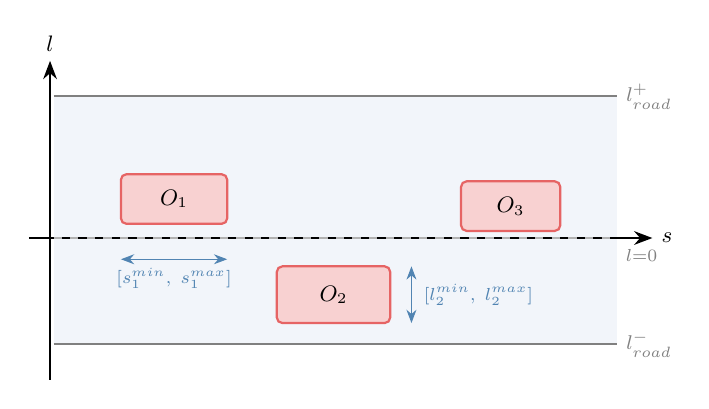
\begin{tikzpicture}[scale=0.9, transform shape]

  % 坐标轴（先画，不被遮挡）
  \draw[-{Stealth}, thick] (-0.3,0) -- (8.5,0) node[right, font=\small\bfseries] {$s$};
  \draw[-{Stealth}, thick] (0,-2.0) -- (0,2.5) node[above, font=\small\bfseries] {$l$};

  % 道路背景（在坐标轴之后，用 scope + opacity 避免遮挡）
  \begin{scope}[on background layer]
    \fill[bglight] (0.05,-1.5) rectangle (8.0,2.0);
  \end{scope}

  % 道路边界
  \draw[gray, thick] (0.05,2.0) -- (8.0,2.0) node[right, font=\footnotesize] {$l_{road}^+$};
  \draw[gray, thick] (0.05,-1.5) -- (8.0,-1.5) node[right, font=\footnotesize] {$l_{road}^-$};

  % 参考线
  \draw[dashed, gray!60] (0.05,0) -- (8.0,0);
  \node[gray, font=\scriptsize, right] at (8.0,-0.25) {$l{=}0$};

  % O1 SL矩形（弯道前段，l > 0）
  \fill[dangerred!30, draw=dangerred, thick, rounded corners=2pt]
    (1.0,0.2) rectangle (2.5,0.9);
  \node[font=\small\bfseries] at (1.75,0.55) {$O_1$};
  \draw[{Stealth}-{Stealth}, thin, deepblue] (1.0,-0.3) -- (2.5,-0.3);
  \node[deepblue, font=\scriptsize, below] at (1.75,-0.3) {$[s_1^{min},\;s_1^{max}]$};

  % O2 SL矩形（弯道中段，l < 0）
  \fill[dangerred!30, draw=dangerred, thick, rounded corners=2pt]
    (3.2,-1.2) rectangle (4.8,-0.4);
  \node[font=\small\bfseries] at (4.0,-0.8) {$O_2$};
  \draw[{Stealth}-{Stealth}, thin, deepblue] (5.1,-1.2) -- (5.1,-0.4);
  \node[deepblue, font=\scriptsize, right] at (5.15,-0.8) {$[l_2^{min},\;l_2^{max}]$};

  % O3 SL矩形（弯道后段，l > 0）
  \fill[dangerred!30, draw=dangerred, thick, rounded corners=2pt]
    (5.8,0.1) rectangle (7.2,0.8);
  \node[font=\small\bfseries] at (6.5,0.45) {$O_3$};

\end{tikzpicture}

\end{center}
\vspace*{\fill}

\clearpage

% ============================================================
% ST约束几何表示
% ============================================================

\vspace*{\fill}
\begin{center}
% 时间有效性约束在 ST 图中的几何表示
% 与 7.2.6 横穿行人示例保持一致：v_ego=8 m/s, s_ped=10 m, τ_k=1.25 s
% 网格：横轴 1 单位 = 0.25 s，纵轴 1 单位 = 2 m
%
% 单一动态障碍物（横穿行人，v_s=0），故 ST boundary 与 SBD 上界都是水平
% Baseline 视角：SBD 把行人 ST boundary 推到 s ≤ 9.75 m 在 t ∈ [0, 1.45] 全时段
% MIKU 视角：PathBoundsDecider 用 τ-shifted 投影避让，SBD 上界恢复为 s_max 附近
%   T 约束保留 ego 不得在 τ_k 之前到达 s_k 的硬性条款，是 path 决策有效性的前提
%
% 本图取 MIKU 视角：SBD 原上界 ≈ s_max（水平线 s≈13），T 引入 (0,0)-(τ_k,s_k) 禁止矩形
\begin{tikzpicture}[scale=0.95, transform shape]
    % 坐标轴
    \draw[->, thick] (0,0) -- (8.6,0) node[right, font=\small\bfseries] {$t$/s};
    \draw[->, thick] (0,0) -- (0,7.6) node[above, font=\small\bfseries] {$s$/m};

    % 浅网格
    \draw[gray!12, very thin] (0,0) grid[step=1] (8,7);

    % 横轴刻度
    \foreach \i/\t in {1/0.25, 2/0.5, 3/0.75, 4/1.0, 5/1.25, 6/1.5, 7/1.75, 8/2.0} {
        \draw (\i, -0.08) -- (\i, 0.08);
        \node[below, font=\footnotesize] at (\i, -0.08) {\t};
    }
    % 纵轴刻度
    \foreach \i/\s in {1/2, 2/4, 3/6, 4/8, 5/10, 6/12, 7/14} {
        \draw (-0.08, \i) -- (0.08, \i);
        \node[left, font=\footnotesize] at (-0.08, \i) {\s};
    }

    % ====== 红色 T 禁止区（t < τ_k 内 s > s_k） ======
    \fill[dangerred!15] (0, 5.0) rectangle (5.0, 7);
    \node[font=\small, dangerred!75!black, align=center] at (2.5, 6.0) {$\mathcal{T}$ 禁止区\\$t{<}\tau_k$ 内 $s{>}s_k$};

    % ====== SBD 原上界：横穿行人 v_s=0，故 SBD 推出的 s_ub 为水平 ======
    %  MIKU 流水线下 path 已绕开行人，SBD 上界趋近 s_max；这里取 s≈13（接近道路尾端示意）
    \draw[deepblue!65, very thick, dashed] (0, 6.5) -- (8, 6.5);
    \node[deepblue!65!black, font=\footnotesize, anchor=south] at (6.0, 6.55) {SBD $s_j^{ub,\text{SBD}}$};
    \node[deepblue!65!black, font=\tiny, anchor=south west] at (5.5, 6.05) {（行人 $v_s{=}0$，水平）};

    % ====== T 引入的水平约束线 s = s_k = 10 ======
    \draw[dangerred, very thick] (0, 5.0) -- (5.0, 5.0);
    \draw[dangerred, thin, dashed] (5.0, 5.0) -- (5.0, 0);

    % 约束点 (τ_k, s_k)
    \filldraw[dangerred] (5.0, 5.0) circle (3pt);
    \node[dangerred, font=\small\bfseries, anchor=south west] at (5.10, 5.10) {$(\tau_k,\,s_k){=}(\PedExampleTauK,\,\PedExampleSk)$};

    % ====== 融合上界 = min(SBD, T) ======
    %  t ∈ [0, τ_k]：T=10 < SBD=13，T 主导，融合上界 = 5（网格）
    %  t = τ_k 跳跃：T 解除，min 跳到 SBD = 6.5（网格）
    %  t > τ_k：SBD 主导，融合 = 6.5
    \draw[lightgreen!70!black, ultra thick] (0, 5.0) -- (5.0, 5.0);
    \draw[lightgreen!70!black, thin, dotted] (5.0, 5.0) -- (5.0, 6.5);
    \draw[lightgreen!70!black, ultra thick] (5.0, 6.5) -- (8, 6.5);
    \node[font=\footnotesize\bfseries, lightgreen!70!black, anchor=west] at (0.2, 4.55) {融合 $s_j^{ub}{=}\min(\mathrm{SBD},\,\mathcal{T})$};

    % ====== 速度曲线 s(t)：贴沿到 (τ_k, s_k)，之后沿融合上界平滑爬升 ======
    \draw[deeppink, very thick, smooth, tension=0.55, -{Stealth}]
        plot[smooth] coordinates {(0,0) (1,1.4) (2,2.8) (3,4.0) (4,4.65) (4.5,4.88) (5,5.0) (5.5,5.6) (6,6.0) (7,6.35) (7.8,6.45)};
    \node[deeppink, font=\small\bfseries, anchor=west] at (1.2, 0.85) {速度曲线 $s(t)$};

    % ====== 约束点坐标轴标注 ======
    \node[dangerred, font=\small] at (5.0, -0.45) {$\tau_k$};
    \node[dangerred, font=\small, anchor=east] at (-0.18, 5.0) {$s_k$};

    % ====== 减速贴边箭头 ======
    \draw[-Stealth, thick, deeppink!75!black] (6.6, 3.7) -- (5.08, 4.92);
    \node[deeppink!75!black, font=\scriptsize\bfseries, anchor=west, align=left] at (6.6, 3.55)
        {贴沿抵 $(\tau_k,s_k)$\\行人随后让出};

    % ====== 图例（轴下方横向一行，无边框，与 fig_corridor_a/b 统一风格） ======
    \begin{scope}[shift={(0,-1.1)}]
        % 第 1 项: T 禁止区
        \fill[dangerred!15] (0.30, -0.07) rectangle (0.65, 0.07);
        \node[font=\tiny, anchor=west] at (0.70, 0.00) {$\mathcal{T}$ 禁止区};

        % 第 2 项: SBD 原上界
        \draw[deepblue!65, very thick, dashed] (2.40, 0.00) -- (2.75, 0.00);
        \node[font=\tiny, anchor=west] at (2.80, 0.00) {SBD 原上界};

        % 第 3 项: 融合 min(·)
        \draw[lightgreen!70!black, ultra thick] (4.45, 0.00) -- (4.80, 0.00);
        \node[font=\tiny, anchor=west] at (4.85, 0.00) {融合 $\min(\cdot)$};

        % 第 4 项: QP 输出 s(t)
        \draw[deeppink, very thick, -{Stealth}] (6.40, 0.00) -- (6.75, 0.00);
        \node[font=\tiny, anchor=west] at (6.80, 0.00) {QP 输出 $s(t)$};
    \end{scope}
\end{tikzpicture}

\end{center}
\vspace*{\fill}

\clearpage

% ============================================================
% 路径规划方法分类树
% ============================================================
\vspace*{\fill}
\begin{center}% 路径规划方法分类树
\begin{tikzpicture}[
    scale=1.0, transform shape,
    lvl1/.style={rectangle, rounded corners=3pt, draw=deepblue, fill=deepblue, text=white, minimum width=3.2cm, minimum height=0.9cm, font=\normalsize\bfseries, align=center},
    lvl2/.style={rectangle, rounded corners=2pt, draw=deepblue, fill=lightblue, minimum width=2.6cm, minimum height=0.8cm, font=\small, align=center},
    methodbox/.style={rectangle, rounded corners=2pt, draw=deepblue!60, fill=bglight, minimum width=2.6cm, font=\footnotesize, align=center, inner sep=6pt},
    methodboxhl/.style={rectangle, rounded corners=2pt, draw=deeppink, fill=lightpink!50, minimum width=2.6cm, font=\footnotesize, align=center, inner sep=6pt},
    hl/.style={rectangle, rounded corners=2pt, draw=deeppink, fill=improvedpink, minimum width=2.6cm, minimum height=0.8cm, font=\small, align=center},
    arr/.style={-Stealth, thick, deepblue},
    arrhl/.style={-Stealth, thick, deeppink},
]

\node[lvl1] (root) at (0,0) {路径规划方法};

\node[lvl2] (g1) at (-6,-1.6) {图搜索方法};
\node[lvl2] (g2) at (-2,-1.6) {采样方法};
\node[hl]   (g3) at (2,-1.6) {优化方法};
\node[lvl2] (g4) at (6,-1.6) {学习方法};

\node[methodbox] (b1) at (-6,-3.8) {A*\\Dijkstra\\D* / Hybrid A*};
\node[methodbox] (b2) at (-2,-3.8) {RRT\\RRT*\\PRM};
\node[methodboxhl] (b3) at (2,-3.8) {QP / iLQR\\Apollo PJPO\\MPC};
\node[methodbox] (b4) at (6,-3.8) {强化学习\\模仿学习\\Transformer};

\draw[arr] (root) -- (g1);
\draw[arr] (root) -- (g2);
\draw[arrhl] (root) -- (g3);
\draw[arr] (root) -- (g4);

\draw[arr] (g1) -- (b1);
\draw[arr] (g2) -- (b2);
\draw[arrhl] (g3) -- (b3);
\draw[arr] (g4) -- (b4);

\node[font=\footnotesize, deeppink] at (2,-5.5) {本文工作所属分支};

\end{tikzpicture}
\end{center}
\vspace*{\fill}
\clearpage

% ============================================================
% 凸 QP 几何
% ============================================================
\vspace*{\fill}
\begin{center}% 凸二次规划几何示意
\begin{tikzpicture}[scale=1.0, transform shape]

% 坐标轴
\draw[->, thick] (-0.3,0) -- (7.2,0) node[right,font=\footnotesize] {$x_1$};
\draw[->, thick] (0,-0.3) -- (0,5.7) node[above,font=\footnotesize] {$x_2$};

% 可行域多边形（浅绿半透明）
\fill[lightgreen, opacity=0.55]
  (1.2,0.6) -- (5.6,0.9) -- (6.4,2.8) -- (4.8,4.6) -- (1.8,4.2) -- (0.8,2.4) -- cycle;
\draw[deepblue, very thick]
  (1.2,0.6) -- (5.6,0.9) -- (6.4,2.8) -- (4.8,4.6) -- (1.8,4.2) -- (0.8,2.4) -- cycle;

\node[deepblue, font=\small\bfseries] at (3.2,3.5) {$\mathcal{F}$ 可行域};
\node[deepblue, font=\footnotesize] at (6.3,0.25) {$a_i^\top x \leq b_i$};

% 目标函数等高线（椭圆族）
\foreach \r in {0.4, 0.85, 1.35, 1.9, 2.5, 3.1} {
  \draw[deeppink!70, thick, rotate around={-18:(3.8,2.4)}]
    (3.8,2.4) ellipse ({\r*1.3} and \r);
}
\node[deeppink!80!black, font=\footnotesize] at (0.6,4.9) {$\frac{1}{2}x^\top P x + q^\top x$ 等值线};

% 无约束最小点
\fill[deeppink] (3.8,2.4) circle (2.2pt);
\node[deeppink, font=\footnotesize, above right=-1pt and -1pt] at (3.8,2.4) {$x^\star_{\text{uncon}}$};

% 约束最优解（在可行域边界上）
\fill[deepblue] (4.85,0.95) circle (3pt);
\draw[deepblue, thick] (4.85,0.95) circle (6pt);
\node[deepblue, font=\footnotesize\bfseries, below=2pt] at (4.85,0.75) {$x^\star$ 最优解};

% 从无约束最优点到有约束最优点的短箭头
\draw[->, thick, gray, dashed] (3.8,2.4) -- (4.75,1.05);

\end{tikzpicture}
\end{center}
\vspace*{\fill}
\clearpage

% ============================================================
% NUDGE 决策效应 子图a
% ============================================================
\vspace*{\fill}\begin{center}\input{fig_nudge_decision_a}\end{center}\vspace*{\fill}\clearpage
% ============================================================
% NUDGE 决策效应 子图b
% ============================================================
\vspace*{\fill}\begin{center}% LEFT_NUDGE 决策对边界影响（子图 b）
% 障碍物在参考线下方，左绕 → 下界被抬高至 v_i = l_i^max + δ
\begin{tikzpicture}[scale=1.0, transform shape]

  % 道路背景
  \fill[bglight] (0,-2.5) rectangle (7.5,2.5);

  % 道路边界
  \draw[gray, thick] (0, 2.5) -- (7.5, 2.5);
  \node[gray, font=\scriptsize, above left] at (7.5, 2.5) {$l_{road}^+$};
  \draw[gray, thick] (0,-2.5) -- (7.5,-2.5);
  \node[gray, font=\scriptsize, below left] at (7.5,-2.5) {$l_{road}^-$};

  % 参考线
  \draw[gray, dashed] (0,0) -- (7.5,0);
  \node[gray, font=\scriptsize, right] at (7.5,0) {$l{=}0$};

  % l 轴
  \draw[-{Stealth}, thick] (0.3,-2.5) -- (0.3,2.8) node[above, font=\footnotesize] {$l$};

  % 障碍物 O_i（参考线下方）
  \fill[dangerred!70, draw=dangerred, thick] (2.5,-1.5) rectangle (4.5,-0.5);
  \node[white, font=\footnotesize\bfseries] at (3.5,-1.0) {$O_i$};

  % 障碍物膨胀虚线框
  \draw[dangerred!70, dashed, thick] (2.2,-1.9) rectangle (4.8,-0.1);
  \node[dangerred!70, font=\scriptsize, right] at (4.9,-1.5) {$+\delta$};

  % 下界 l-(s)：从道路下界 → 抬高到 v_i → 恢复道路下界
  % 与道路边界连起来
  \draw[deepblue, very thick]
    (0,-2.5) -- (2.2,-2.5) -- (2.2,-0.1) -- (4.8,-0.1) -- (4.8,-2.5) -- (7.5,-2.5);
  \node[deepblue, font=\small] at (3.5,0.3) {$l^-(s) = v_i$};

  % 上界 l+(s)：保持道路上界不变
  \draw[deeppink, very thick, dashed]
    (0, 2.5) -- (7.5, 2.5);
  \node[deeppink, font=\small, below left] at (7.5, 2.3) {$l^+(s)$};

  % v_i 标注
  \draw[{Stealth}-{Stealth}, thin, deepblue] (5.2,-2.5) -- (5.2,-0.1);
  \node[deepblue, font=\scriptsize, right] at (5.3,-1.3) {被压缩};

  % 自车轨迹：起点终点在 l=0，向上远离障碍物弯曲
  \draw[deepblue, very thick, -{Stealth}]
    plot[smooth, tension=0.55] coordinates
      {(0.5, 0) (1.5, 0.3) (2.5, 0.8) (3.5, 1.0) (4.5, 0.8) (5.5, 0.3) (6.5, 0)};
  \node[deepblue, font=\footnotesize\bfseries, above] at (3.5,1.2) {自车轨迹};

\end{tikzpicture}
\end{center}\vspace*{\fill}\clearpage

% ============================================================
% Planning 数据流
% ============================================================
\vspace*{\fill}
\begin{center}% Planning 模块单周期数据流
\begin{tikzpicture}[
    scale=0.85, transform shape,
    >=Stealth,
    % 输入小盒
    inp/.style={rectangle, rounded corners=1pt, draw=deepblue,
                fill=inputyellow, minimum width=1.65cm, minimum height=0.6cm,
                font=\footnotesize, align=center, inner sep=2pt},
    % 层内子步骤
    step box/.style={rectangle, rounded corners=2pt, draw=deepblue,
                     fill=lightblue, minimum width=1.8cm, minimum height=0.6cm,
                     font=\footnotesize, align=center, inner sep=2pt},
    % 改进层子步骤
    step imp/.style={rectangle, rounded corners=2pt, draw=deeppink,
                     fill=improvedpink, minimum width=1.8cm, minimum height=0.6cm,
                     font=\footnotesize, align=center, inner sep=2pt},
    % 层背景
    layer bg/.style={rectangle, rounded corners=6pt, fill=bglight,
                     draw=deepblue!50, inner sep=8pt},
    % 改进层背景
    layer imp/.style={rectangle, rounded corners=6pt, fill=improvedpink!15,
                      draw=deeppink!60, inner sep=8pt},
    % 输出节点
    out box/.style={rectangle, rounded corners=3pt, draw=deeppink,
                    fill=outputpink, minimum width=4cm, minimum height=0.7cm,
                    font=\small\bfseries, align=center},
]

% ===================== 输入层 (y = 0) =====================
\node[inp] (i1) at (-4,   0) {Prediction\\[-1pt]Obstacles};
\node[inp] (i2) at (-2,   0) {Chassis};
\node[inp] (i3) at ( 0,   0) {Localization};
\node[inp] (i4) at ( 2,   0) {TrafficLight};
\node[inp] (i5) at ( 4,   0) {Planning\\[-1pt]Command};
\node[font=\small, text=deepblue, anchor=east] at (-5.2, 0) {Cyber RT 输入};

% 汇聚点
\coordinate (merge) at (0, -1.0);
\foreach \i in {i1,i2,i3,i4,i5}{
    \draw[flow] (\i.south) -- (merge);
}

% ===================== Layer 1: Proc() (y = -2.2) =====================
\node[step box] (p1) at (-2.8, -2.2) {CheckRerouting};
\node[step box] (p2) at ( 0,   -2.2) {构建 LocalView};
\node[step box] (p3) at ( 2.8, -2.2) {CheckInput};

\draw[flow] (p1) -- (p2);
\draw[flow] (p2) -- (p3);

% 隐藏锚点，使三层 fit 宽度一致
\coordinate (L1pad-l) at (-4.4, -2.2);
\coordinate (L1pad-r) at ( 4.4, -2.2);

\begin{scope}[on background layer]
    \node[layer bg, fit=(L1pad-l)(L1pad-r)(p1)(p2)(p3),
          label={[font=\small, text=deepblue, anchor=east]left:Proc()}] (L1) {};
\end{scope}

\draw[flow, line width=1.2pt] (merge) -- (L1.north);

% ===================== Layer 2: RunOnce() (y = -4.2) =====================
\node[step box] (r1) at (-3.4, -4.2) {VehicleState\\[-1pt]更新};
\node[step box] (r2) at (-1.1, -4.2) {参考线平滑};
\node[step box] (r3) at ( 1.2, -4.2) {轨迹拼接};
\node[step box] (r4) at ( 3.4, -4.2) {Frame\\[-1pt]初始化};

\draw[flow] (r1) -- (r2);
\draw[flow] (r2) -- (r3);
\draw[flow] (r3) -- (r4);

\begin{scope}[on background layer]
    \node[layer bg, fit=(r1)(r2)(r3)(r4),
          label={[font=\small, text=deepblue, anchor=east]left:RunOnce()}] (L2) {};
\end{scope}

\draw[flow, line width=1.2pt] (L1.south) -- (L2.north);

% ===================== Layer 3: Plan() (y = -6.2) =====================
\node[step imp] (s1) at (-3.4, -6.2) {Scenario\\[-1pt]Manager};
\node[step imp] (s2) at (-1.1, -6.2) {Scenario\\[-1pt]::Process};
\node[step imp] (s3) at ( 1.2, -6.2) {Stage\\[-1pt]::Process};
\node[step imp] (s4) at ( 3.4, -6.2) {Task\\[-1pt]::Execute};

\draw[flowimp] (s1) -- (s2);
\draw[flowimp] (s2) -- (s3);
\draw[flowimp] (s3) -- (s4);

\begin{scope}[on background layer]
    \node[layer imp, fit=(s1)(s2)(s3)(s4),
          label={[font=\small, text=deeppink, anchor=east]left:Plan()}] (L3) {};
\end{scope}

\node[font=\footnotesize, text=deeppink!80!black, anchor=west] at (L3.east) {~~核心执行层};

\draw[flowimp, line width=1.2pt] (L2.south) -- (L3.north);

% ===================== 输出 (y = -8.0) =====================
\node[out box] (output) at (0, -8.0) {ADCTrajectory};

\draw[flowimp, line width=1.2pt] (L3.south) -- (output.north);

\end{tikzpicture}
\end{center}
\vspace*{\fill}
\clearpage

% ============================================================
% 路径-速度解耦
% ============================================================
\vspace*{\fill}
\begin{center}% 路径-速度解耦三阶段架构（左→右流水线）
\begin{tikzpicture}[
    scale=0.82, transform shape,
    >=Stealth,
    inp/.style={rectangle, rounded corners=1pt, draw=deepblue,
                fill=inputyellow, minimum width=1.6cm, minimum height=0.55cm,
                font=\footnotesize, align=center, inner sep=2pt},
    sl box/.style={rectangle, rounded corners=2pt, draw=deepblue,
                   fill=white, minimum width=2.8cm, minimum height=0.55cm,
                   font=\footnotesize, align=center, inner sep=2pt},
    st box/.style={rectangle, rounded corners=2pt, draw=deepblue,
                   fill=white, minimum width=2.8cm, minimum height=0.55cm,
                   font=\footnotesize, align=center, inner sep=2pt},
    sl bg/.style={rectangle, rounded corners=6pt, fill=lightblue!40,
                  draw=deepblue!60, inner sep=8pt},
    st bg/.style={rectangle, rounded corners=6pt, fill=skyblue!35,
                  draw=deepblue!60, inner sep=8pt},
    stglabel/.style={font=\footnotesize\bfseries, text=deepblue},
    out box/.style={rectangle, rounded corners=3pt, draw=deeppink,
                    fill=outputpink, minimum width=2.4cm, minimum height=0.7cm,
                    font=\small\bfseries, align=center},
]

% ==================== 左列：输入（与其他阶段间隔等价） ====================
\node[inp] (i1) at (0.9, 1.5)  {参考线};
\node[inp] (i2) at (0.9, 0.5)  {感知障碍物};
\node[inp] (i3) at (0.9, -0.5) {预测轨迹};
\node[inp] (i4) at (0.9, -1.5) {车辆状态};

% ==================== 阶段一：SL路径规划 (x=5) ====================
\node[sl box] (s1a) at (5, 0.85)  {PathBoundsDecider\\[-1pt]构建SL边界};
\node[sl box] (s1b) at (5, -0.85) {PiecewiseJerkPath-\\[-1pt]Optimizer\enspace QP求解};

\draw[flow] (s1a) -- (s1b);

\coordinate (s1pad-t) at (5, 1.5);
\coordinate (s1pad-b) at (5, -1.5);

\begin{scope}[on background layer]
    \node[sl bg, fit=(s1pad-t)(s1pad-b)(s1a)(s1b)] (S1) {};
\end{scope}

\node[stglabel, anchor=south] at (S1.north) {阶段一：路径规划};
\node[font=\scriptsize, text=deepblue!70, anchor=north] at (S1.south) {SL空间};


% ==================== 阶段二：DP速度搜索 (x=10) ====================
\node[st box] (s2a) at (10, 0.85)  {ST图网格构建};
\node[st box] (s2b) at (10, -0.85) {DP启发式搜索};

\draw[flow] (s2a) -- (s2b);

\coordinate (s2pad-t) at (10, 1.5);
\coordinate (s2pad-b) at (10, -1.5);

\begin{scope}[on background layer]
    \node[st bg, fit=(s2pad-t)(s2pad-b)(s2a)(s2b)] (S2) {};
\end{scope}

\node[stglabel, anchor=south] at (S2.north) {阶段二：速度搜索};
\node[font=\scriptsize, text=deepblue!70, anchor=north] at (S2.south) {ST空间};

% ==================== 阶段三：QP速度优化 (x=15) ====================
\node[st box] (s3a) at (15, 0.85) {PiecewiseJerkSpeed-\\[-1pt]Optimizer};
\node[st box] (s3b) at (15, -0.85){QP精细优化};

\draw[flow] (s3a) -- (s3b);

\coordinate (s3pad-t) at (15, 1.5);
\coordinate (s3pad-b) at (15, -1.5);

\begin{scope}[on background layer]
    \node[st bg, fit=(s3pad-t)(s3pad-b)(s3a)(s3b)] (S3) {};
\end{scope}

\node[stglabel, anchor=south] at (S3.north) {阶段三：速度优化};
\node[font=\scriptsize, text=deepblue!70, anchor=north] at (S3.south) {ST空间};

% ==================== 输出 (x=19.5) ====================
\node[out box] (output) at (19.5, 0) {ADCTrajectory};

% ==================== 输入 → 阶段一 ====================
\draw[flow] (i1.east) -- (S1.west);
\draw[flow] (i2.east) -- (S1.west);
\draw[flow] (i3.east) -- (S1.west);
\draw[flow] (i4.east) -- (S1.west);

% ==================== 阶段间箭头 ====================
\draw[flow] (S1.east) -- node[above, font=\scriptsize, text=deepblue] {$l(s)$ 路径}
                          node[below, font=\scriptsize, text=deeppink] {SL$\,\to\,$ST} (S2.west);

\draw[flow] (S2.east) -- node[above, font=\scriptsize, text=deepblue] {速度走廊} (S3.west);

\draw[flow] (S3.east) -- (output.west);

\end{tikzpicture}
\end{center}
\vspace*{\fill}
\clearpage

% ============================================================
% PathBoundsDecider 流程
% ============================================================
\vspace*{\fill}
\begin{center}% PathBoundsDecider 构建流程图
\begin{tikzpicture}[
    scale=1.0, transform shape,
    box/.style={rectangle, rounded corners=3pt, draw=deepblue, fill=lightblue, minimum width=4.2cm, minimum height=0.9cm, font=\small, align=center},
    boximp/.style={rectangle, rounded corners=3pt, draw=deeppink, fill=improvedpink, minimum width=4.2cm, minimum height=0.9cm, font=\small, align=center},
    dec/.style={diamond, aspect=2, draw=deepblue, fill=skyblue, minimum width=4.2cm, minimum height=0.9cm, font=\small, align=center, inner sep=1pt},
    term/.style={rectangle, rounded corners=8pt, draw=deeppink, fill=outputpink, minimum width=3.2cm, minimum height=0.8cm, font=\small\bfseries, align=center},
    arr/.style={-Stealth, thick, deepblue},
    arrno/.style={-Stealth, thick, dangerred},
]

\node[term, fill=inputyellow, draw=deepblue] (start) at (0,7.0) {输入 障碍物集合};

\node[box] (init) at (0,5.2) {初始化路径边界为车道边};

\node[dec] (loop) at (0,3.2) {遍历障碍物 $O_i$};

\node[box] (decide) at (-5,1.2) {判断避让方向\\ $d_i\in\{L,R\}$};

\node[boximp] (update) at (0,1.2) {更新 $l^+$ 或 $l^-$};

\node[dec] (check) at (0,-1.2) {通行带宽 $W(s) < W_{\text{ego}}$?};

\node[term, fill=dangerred!40, draw=dangerred] (blocked) at (5.5,-1.2) {BLOCKED};
\node[term] (ok) at (0,-3.4) {输出 path\_boundary};

% 流
\draw[arr] (start) -- (init);
\draw[arr] (init) -- (loop);
\draw[arr] (loop) -- (decide);
\draw[arr] (decide) -- (update);
\draw[arr] (update) -- (check);
\draw[arrno] (check) -- node[above, font=\footnotesize, dangerred] {是} (blocked);
\draw[arr] (check) -- node[left, font=\footnotesize, deepblue] {否} (ok);

% 反馈回 loop（遍历下一个）
\draw[arr] (update.east) -- ++(1.8,0) |- (loop.east);
\node[font=\scriptsize, deepblue] at (2.6,2.2) {下一个 $O_{i+1}$};

% 侧注
\node[font=\footnotesize, align=left, anchor=north west, deeppink!80!black] at (3.8,4.5)
  {核心问题：决策逐障碍物独立做出，\\后续障碍物无法修正前序决策。};

\end{tikzpicture}
\end{center}
\vspace*{\fill}
\clearpage

% ============================================================
% 三问题示意 子图a
% ============================================================
\vspace*{\fill}\begin{center}% 问题一 安全裕度一刀切（子图 a）
\begin{tikzpicture}[scale=0.95, transform shape]
  % 统一边界框：与子图 b/c 对齐
  \useasboundingbox (0,-1.9) rectangle (6.0,1.9);

  % 道路
  \fill[bglight] (0,-1.8) rectangle (6.0,1.8);
  \draw[deepblue, thick] (0,-1.8) -- (6.0,-1.8);
  \draw[deepblue, thick] (0, 1.8) -- (6.0, 1.8);
  \draw[deepblue, dashed, thin] (0,0) -- (6.0,0);
  \node[gray, font=\tiny, left] at (0,0) {$l{=}0$};

  % 路锥（小三角，低威胁）
  \fill[dangerred!70] (2.5,-0.15) -- (2.9,-0.15) -- (2.7,0.2) -- cycle;
  \node[font=\scriptsize, dangerred!70!black, above] at (2.7,0.3) {路锥};

  % 膨胀框（统一 δ=1.2m，和大车一样大）
  \draw[dangerred!70, dashed, thick] (1.8,-0.9) rectangle (3.6,0.9);

  % 垂直箭头标注膨胀距离
  \draw[{Stealth}-{Stealth}, dangerred!70, thick] (3.9, 0.2) -- (3.9, 0.9);
  \node[dangerred!70!black, font=\scriptsize, right] at (4.0, 0.55) {$\delta{=}1.2$m};
  \draw[{Stealth}-{Stealth}, dangerred!70, thick] (3.9, -0.15) -- (3.9, -0.9);
  \node[dangerred!70!black, font=\scriptsize, right] at (4.0, -0.52) {$\delta{=}1.2$m};

  % 通行带被压缩标注（道路下方）
  \draw[{Stealth}-{Stealth}, lightgreen!60!black, thick] (0.8, -0.9) -- (0.8, -1.8);
  \node[font=\scriptsize, lightgreen!60!black, left] at (0.7, -1.35) {残余};

  \draw[{Stealth}-{Stealth}, lightgreen!60!black, thick] (5.2, -0.9) -- (5.2, -1.8);
  \node[font=\scriptsize, lightgreen!60!black, right] at (5.3, -1.35) {残余};

  % 标注放到道路底部残余通道内（y∈[-1.8,-0.9]）
  \node[font=\scriptsize\bfseries, lightgreen!60!black] at (3.0,-1.35) {通行带被过度压缩};

\end{tikzpicture}
\end{center}\vspace*{\fill}\clearpage
% ============================================================
% 三问题示意 子图b
% ============================================================
\vspace*{\fill}\begin{center}% 问题二 独立决策矛盾（子图 b）
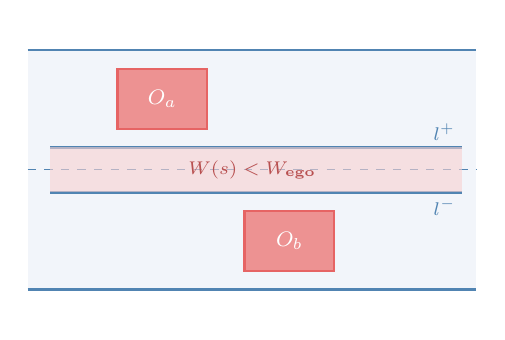
\begin{tikzpicture}[scale=0.95, transform shape]
  % 统一边界框：与子图 a/c 对齐
  \useasboundingbox (0,-1.9) rectangle (6.0,1.9);

  \fill[bglight] (0,-1.6) rectangle (6.0,1.6);
  \draw[deepblue, thick] (0,-1.6) -- (6.0,-1.6);
  \draw[deepblue, thick] (0, 1.6) -- (6.0, 1.6);
  \draw[deepblue, dashed, thin] (0,0) -- (6.0,0);

  \fill[obsstatic] (1.2,0.55) rectangle (2.4,1.35);
  \node[white, font=\footnotesize\bfseries] at (1.8,0.95) {$O_a$};

  \fill[obsstatic] (2.9,-1.35) rectangle (4.1,-0.55);
  \node[white, font=\footnotesize\bfseries] at (3.5,-0.95) {$O_b$};

  \draw[deepblue, very thick] (0.3,0.3) -- (5.8,0.3);
  \node[deepblue, font=\scriptsize, right] at (5.3,0.5) {$l^+$};

  \draw[deepblue, very thick] (0.3,-0.3) -- (5.8,-0.3);
  \node[deepblue, font=\scriptsize, right] at (5.3,-0.5) {$l^-$};

  \fill[dangerred!30, opacity=0.6] (0.3,-0.3) rectangle (5.8,0.3);
  \node[dangerred!80!black, font=\scriptsize\bfseries] at (3.0,0) {$W(s)<W_{\text{ego}}$};
\end{tikzpicture}
\end{center}\vspace*{\fill}\clearpage
% ============================================================
% 三问题示意 子图c
% ============================================================
\vspace*{\fill}\begin{center}% 问题三 动态障碍物排除（子图 c）
\begin{tikzpicture}[scale=0.95, transform shape]
  % 统一边界框：与子图 a/b 对齐
  \useasboundingbox (0,-1.9) rectangle (6.0,1.9);

  % 道路
  \fill[bglight] (0,-1.8) rectangle (6.0,1.8);
  \draw[deepblue, thick] (0,-1.8) -- (6.0,-1.8);
  \draw[deepblue, thick] (0, 1.8) -- (6.0, 1.8);
  \draw[deepblue, dashed, thin] (0,0) -- (6.0,0);

  % 行人（动态障碍物）
  \fill[obsdyn] (3.5,0.1) rectangle (4.0,0.7);
  \draw[-Stealth, thick, dangerred] (3.75,0.7) -- (3.75,1.4);
  \node[font=\scriptsize, dangerred!70!black, right] at (4.1,1.15) {行人 1.2m/s};

  % Path阶段排除标记：× 叠在行人上，文字移到道路内右上方
  \node[dangerred, font=\Large, opacity=0.85] at (3.75,0.4) {\textbf{$\times$}};
  \node[font=\scriptsize, dangerred!80!black, right] at (4.1,0.4) {Path阶段排除};

  % 自车
  \fill[deepblue] (0.6,-0.35) rectangle (1.2,0.35);
  \node[deepblue, font=\tiny, below] at (0.9,-0.4) {自车};
  \draw[-Stealth, thick, deepblue] (1.3,0) -- (3.2,0);
  \node[font=\scriptsize, deepblue, above] at (2.25,0.05) {8 m/s};

  % Speed阶段才发现标注
  \draw[dangerred, very thick, dashed] (3.2,-0.6) rectangle (4.3,0.9);
  \node[dangerred, font=\scriptsize\bfseries] at (2.2,-1.25) {Speed阶段才发现};
  \draw[dangerred, thin] (3.0,-1.15) -- (3.2,-0.7);

\end{tikzpicture}
\end{center}\vspace*{\fill}\clearpage

% ============================================================
% 安全距离压缩
% ============================================================
\vspace*{\fill}
\begin{center}% 路锥场景：差异化 d_buf vs 统一 d_buf 对比
\begin{tikzpicture}[scale=1.0, transform shape]

% ============================================================
% 子图 (a)：差异化 d_buf=0.15m，恰好可通行
% ============================================================
\begin{scope}[shift={(0,0)}]
  % 背景
  \fill[bglight] (0,-2.3) rectangle (7.0,2.3);

  % 道路边界 ±1.875m
  \draw[deepblue, very thick] (0,-1.875) -- (7.0,-1.875);
  \draw[deepblue, very thick] (0, 1.875) -- (7.0, 1.875);
  \draw[deepblue, dashed, thin] (0,0) -- (7.0,0);

  % 车道宽度标注
  \draw[{Stealth}-{Stealth}, thin, deepblue] (0.3,-1.875) -- (0.3,1.875);
  \node[font=\scriptsize, deepblue, rotate=90] at (0.6,0) {车道 3.75m};

  % 路锥（宽0.3m，高0.3m，中心在 (3.25, -0.225)）
  % 横向 l: [-0.375, -0.075]，纵向 s: [3.1, 3.4]
  \fill[dangerred!70, draw=dangerred, thick] (3.1,-0.375) rectangle (3.4,-0.075);
  \node[white, font=\tiny\bfseries] at (3.25,-0.225) {锥};

  % 缓冲区 d_buf=0.15m（四周等距膨胀 0.15m）
  % l: [-0.375-0.15, -0.075+0.15] = [-0.525, 0.075]
  % s: [3.1-0.15, 3.4+0.15] = [2.95, 3.55]
  \draw[dangerred!70, dashed, thick] (2.95,-0.525) rectangle (3.55,0.075);
  \node[dangerred!70!black, font=\scriptsize, anchor=west] at (3.7,-0.225)
    {$\delta{=}0.15$m};

  % 膨胀距离标注（垂直）
  \draw[{Stealth}-{Stealth}, dangerred!60, thin] (2.8,-0.375) -- (2.8,-0.525);
  \node[dangerred!60, font=\tiny, left] at (2.75,-0.45) {0.15};
  \draw[{Stealth}-{Stealth}, dangerred!60, thin] (2.8,-0.075) -- (2.8,0.075);
  \node[dangerred!60, font=\tiny, left] at (2.75,0.0) {0.15};

  % 通行区域 [0.075, 1.875]（绿色填充）
  \fill[lightgreen, opacity=0.25] (1.0,0.075) rectangle (5.5,1.875);

  % 自车（宽1.8m = y方向，长4.5m = x方向，1:1比例）
  \fill[deepblue, opacity=0.3] (1.0,0.075) rectangle (5.5,1.875);
  \draw[deepblue, thick, rounded corners=2pt] (1.0,0.075) rectangle (5.5,1.875);
  \node[deepblue, font=\scriptsize\bfseries] at (3.25,0.975) {自车};

  % 净间距标注
  \draw[{Stealth}-{Stealth}, thick, lightgreen!60!black] (6.2,0.075) -- (6.2,1.875);
  \node[font=\scriptsize, lightgreen!60!black, anchor=west] at (6.3,0.975) {1.80m};
  \node[font=\scriptsize, lightgreen!60!black, anchor=west] at (6.3,0.55) {$= W_{\mathrm{ego}}$};

  \node[lightgreen!60!black, font=\normalsize\bfseries] at (1.5,-2.1) {\checkmark};

  % 子图标题
  \node[font=\small\bfseries, align=center] at (3.5,-2.7)
    {(a) $\delta{=}0.15$m（差异化），恰好可通行};
\end{scope}

% ============================================================
% 子图 (b)：Apollo d_buf=0.3m，BLOCKED
% ============================================================
\begin{scope}[shift={(8.5,0)}]
  % 背景
  \fill[bglight] (0,-2.3) rectangle (7.0,2.3);

  % 道路边界 ±1.875m
  \draw[deepblue, very thick] (0,-1.875) -- (7.0,-1.875);
  \draw[deepblue, very thick] (0, 1.875) -- (7.0, 1.875);
  \draw[deepblue, dashed, thin] (0,0) -- (7.0,0);

  % 车道宽度标注
  \draw[{Stealth}-{Stealth}, thin, deepblue] (0.3,-1.875) -- (0.3,1.875);
  \node[font=\scriptsize, deepblue, rotate=90] at (0.6,0) {车道 3.75m};

  % 路锥（同样大小）
  \fill[dangerred!70, draw=dangerred, thick] (3.1,-0.375) rectangle (3.4,-0.075);
  \node[white, font=\tiny\bfseries] at (3.25,-0.225) {锥};

  % 缓冲区 d_buf=0.3m（四周等距膨胀 0.3m）
  % l: [-0.375-0.3, -0.075+0.3] = [-0.675, 0.225]
  % s: [3.1-0.3, 3.4+0.3] = [2.8, 3.7]
  \draw[dangerred!70, dashed, thick] (2.8,-0.675) rectangle (3.7,0.225);
  \node[dangerred!70!black, font=\scriptsize, anchor=west] at (3.85,-0.225)
    {$\delta{=}0.3$m};

  % 膨胀距离标注
  \draw[{Stealth}-{Stealth}, dangerred!60, thin] (2.6,-0.375) -- (2.6,-0.675);
  \node[dangerred!60, font=\tiny, left] at (2.55,-0.525) {0.3};
  \draw[{Stealth}-{Stealth}, dangerred!60, thin] (2.6,-0.075) -- (2.6,0.225);
  \node[dangerred!60, font=\tiny, left] at (2.55,0.075) {0.3};

  % 上方不足区域 [0.225, 1.875] = 1.65m
  \fill[dangerred, opacity=0.12] (1.0,0.225) rectangle (5.5,1.875);
  % 下方不足区域 [-1.875, -0.675] = 1.2m
  \fill[dangerred, opacity=0.12] (1.0,-1.875) rectangle (5.5,-0.675);

  % 上方净间距
  \draw[{Stealth}-{Stealth}, thick, dangerred] (5.7,0.225) -- (5.7,1.875);
  \node[font=\scriptsize, dangerred, anchor=west] at (5.8,1.05) {1.65m};
  \node[font=\scriptsize, dangerred, anchor=west] at (5.8,0.65) {$< W_{\mathrm{ego}}$};

  % 下方净间距
  \draw[{Stealth}-{Stealth}, thick, dangerred] (5.7,-1.875) -- (5.7,-0.675);
  \node[font=\scriptsize, dangerred, anchor=west] at (5.8,-1.275) {1.20m};
  \node[font=\scriptsize, dangerred, anchor=west] at (5.8,-1.6) {$< W_{\mathrm{ego}}$};

  % BLOCKED
  \draw[dangerred, ultra thick] (2.5,1.0) -- (4.0,-1.0);
  \draw[dangerred, ultra thick] (2.5,-1.0) -- (4.0,1.0);
  \node[dangerred, font=\small\bfseries] at (3.25,-2.1) {BLOCKED};

  % 子图标题
  \node[font=\small\bfseries, align=center] at (3.5,-2.7)
    {(b) $\delta{=}0.3$m（统一），BLOCKED};
\end{scope}

\end{tikzpicture}
\end{center}
\vspace*{\fill}
\clearpage

% ============================================================
% 动态障碍物时变排除 子图a
% ============================================================
\vspace*{\fill}\begin{center}% 动态障碍物排除 t=0 时刻（子图 a）
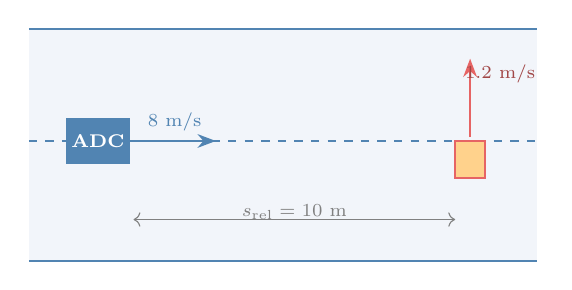
\begin{tikzpicture}[scale=0.95, transform shape]
  \fill[bglight] (0,-1.3) rectangle (6.8,1.8);
  \draw[deepblue, thick] (0,-1.3) -- (6.8,-1.3);
  \draw[deepblue, thick] (0, 1.8) -- (6.8, 1.8);
  \draw[deepblue, dashed, thin] (0,0.3) -- (6.8,0.3);

  \fill[egopt] (0.5,0) rectangle (1.35,0.6);
  \node[white, font=\scriptsize\bfseries] at (0.925,0.3) {ADC};
  \draw[-Stealth, thick, deepblue] (1.4,0.3) -- (2.5,0.3);
  \node[font=\scriptsize, deepblue] at (1.95,0.55) {8 m/s};

  \fill[obsdyn] (5.7,-0.2) rectangle (6.1,0.3);
  \draw[-Stealth, thick, dangerred] (5.9,0.35) -- (5.9,1.4);
  \node[font=\scriptsize, dangerred!70!black] at (6.3,1.2) {1.2 m/s};

  \draw[<->, thin, gray] (1.4,-0.75) -- (5.7,-0.75);
  \node[font=\scriptsize, gray] at (3.55,-0.65) {$s_{\text{rel}}=10$ m};
\end{tikzpicture}
\end{center}\vspace*{\fill}\clearpage
% ============================================================
% 动态障碍物时变排除 子图b
% ============================================================
\vspace*{\fill}\begin{center}% 动态障碍物排除 t=0.625s（子图 b）
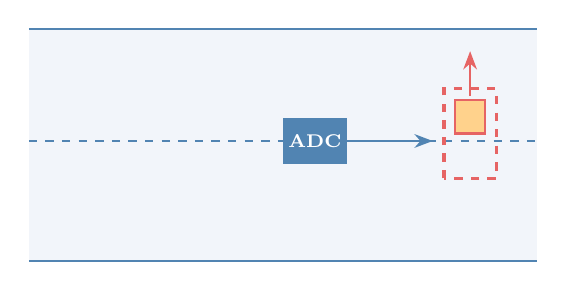
\begin{tikzpicture}[scale=0.95, transform shape]
  \fill[bglight] (0,-1.3) rectangle (6.8,1.8);
  \draw[deepblue, thick] (0,-1.3) -- (6.8,-1.3);
  \draw[deepblue, thick] (0, 1.8) -- (6.8, 1.8);
  \draw[deepblue, dashed, thin] (0,0.3) -- (6.8,0.3);

  \fill[egopt] (3.4,0) rectangle (4.25,0.6);
  \node[white, font=\scriptsize\bfseries] at (3.825,0.3) {ADC};
  \draw[-Stealth, thick, deepblue] (4.3,0.3) -- (5.4,0.3);

  \fill[obsdyn] (5.7,0.4) rectangle (6.1,0.85);
  \draw[-Stealth, thick, dangerred] (5.9,0.9) -- (5.9,1.5);

  \draw[dangerred, very thick, dashed] (5.55,-0.2) rectangle (6.25,1.0);
\end{tikzpicture}
\end{center}\vspace*{\fill}\clearpage
% ============================================================
% 动态障碍物时变排除 子图c
% ============================================================
\vspace*{\fill}\begin{center}% 动态障碍物排除 t=1.25s（子图 c）
\begin{tikzpicture}[scale=0.95, transform shape]
  \fill[bglight] (0,-1.3) rectangle (6.8,1.8);
  \draw[deepblue, thick] (0,-1.3) -- (6.8,-1.3);
  \draw[deepblue, thick] (0, 1.8) -- (6.8, 1.8);
  \draw[deepblue, dashed, thin] (0,0.3) -- (6.8,0.3);

  \fill[egopt, opacity=0.3] (0.5,0) rectangle (1.35,0.6);
  \node[gray, font=\scriptsize] at (0.925,0.3) {$t=0$};

  \fill[egopt] (5.7,0) rectangle (6.55,0.6);
  \node[white, font=\scriptsize\bfseries] at (6.125,0.3) {ADC};

  \fill[obsdyn] (5.7,1.3) rectangle (6.1,1.75);
  \node[font=\scriptsize, dangerred!70!black, above] at (5.9,1.8) {已穿过};

  \fill[bandok] (1.5,0.05) rectangle (5.6,0.55);
  \node[font=\scriptsize, lightgreen!50!black] at (3.5,0.3) {路径已打开};
\end{tikzpicture}
\end{center}\vspace*{\fill}\clearpage

% ============================================================
% u_i/v_i 几何定义
% ============================================================
\vspace*{\fill}
\begin{center}% u_i / v_i 几何定义图
\begin{tikzpicture}[scale=1.0, transform shape]

% 坐标系（先画，不被遮挡）
\draw[->, thick] (0,0) -- (9.7,0) node[right,font=\footnotesize] {$s$};
\draw[->, thick] (0,-2.5) -- (0,3.3) node[above,font=\footnotesize] {$l$};

% 道路背景带（与其他 SL 图统一）
\begin{scope}[on background layer]
  \fill[bglight] (0.05,-2.3) rectangle (9.3,3.0);
\end{scope}

% 道路边界
\draw[gray, thick] (0.05,3.0) -- (9.3,3.0) node[right, font=\footnotesize] {$l_{road}^+$};
\draw[gray, thick] (0.05,-2.3) -- (9.3,-2.3) node[right, font=\footnotesize] {$l_{road}^-$};

% 参考线 l=0
\draw[dashed, gray!60] (0.05,0) -- (9.3,0);
\node[gray, font=\scriptsize, right] at (9.3,-0.25) {$l{=}0$};

% 障碍物矩形 [s_i^-, s_i^+] x [l_i^-, l_i^+]
\fill[obsstatic] (3,-0.8) rectangle (6,1.2);
\node[white, font=\small\bfseries] at (4.5,0.2) {$O_i$};

% s 标注（紧贴障碍物底边，不与轨迹干扰）
\node[font=\scriptsize] at (3,-0.55) {$s_i^-$};
\node[font=\scriptsize] at (6,-0.55) {$s_i^+$};

% l 标注（右侧引线）
\draw[-, thin, gray] (6,-0.8) -- (7.8,-0.8);
\draw[-, thin, gray] (6, 1.2) -- (7.8, 1.2);
\node[font=\scriptsize, anchor=west] at (7.8,-0.8) {$l_i^-$};
\node[font=\scriptsize, anchor=west] at (7.8, 1.2) {$l_i^+$};

% 安全裕度扩展
\draw[obsbuf] (3,-1.4) rectangle (6,1.8);
\draw[<->, thin, dangerred] (2.5,-0.8) -- (2.5,-1.4);
\node[dangerred, font=\scriptsize, left] at (2.5,-1.1) {$\delta$};
\draw[<->, thin, dangerred] (2.5,1.2) -- (2.5,1.8);
\node[dangerred, font=\scriptsize, left] at (2.5,1.5) {$\delta$};

% u_i 线（下方安全边界）
\draw[deepblue, very thick] (3,-1.4) -- (6,-1.4);
\node[deepblue, font=\scriptsize, anchor=west] at (6.2,-1.4) {$u_i = l_i^- - \delta$};

% v_i 线（上方安全边界）
\draw[deeppink, very thick] (3,1.8) -- (6,1.8);
\node[deeppink, font=\scriptsize, anchor=west] at (6.2,1.8) {$v_i = l_i^+ + \delta$};

% 右绕示意路径（起终点在参考线 l=0，与 u_i 保持明显间距）
\draw[deepblue, very thick, densely dashed]
  plot[smooth, tension=0.55] coordinates {(0.5,0) (1.2,-0.6) (2.0,-1.6) (4.5,-2.0) (7.0,-1.6) (7.8,-0.6) (8.5,0)};
\fill[deepblue] (0.5,0) circle (2.5pt);
\node[deepblue, font=\scriptsize] at (1.5,-1.2) {右绕轨迹};

% 左绕示意路径（对称，与 v_i 保持明显间距）
\draw[deeppink, very thick, densely dashed]
  plot[smooth, tension=0.55] coordinates {(0.5,0) (1.2,0.6) (2.0,1.6) (4.5,2.6) (7.0,1.6) (7.8,0.6) (8.5,0)};
\fill[deeppink] (0.5,0) circle (2.5pt);
\node[deeppink, font=\scriptsize] at (4.5,2.8) {左绕轨迹};

\end{tikzpicture}
\end{center}
\vspace*{\fill}
\clearpage

% ============================================================
% 最大间隙定理图证
% ============================================================
\vspace*{\fill}
\begin{center}% 引理1+定理1 几何图证（1D 横向数轴）
\begin{tikzpicture}[scale=1.0, transform shape]

% 障碍物位置设计: g₂ 为最大间隙
% O₁@1.5, O₂@3.0, O₃@6.5, O₄@8.0 (中心)
% 半宽 0.35, δ 扩展 0.55
% l_road⁻=0, l_road⁺=9.5

% === 上图: 排序后的障碍物横向投影 ===

% 道路区域淡色背景（先画，避免盖住坐标轴）
\fill[bglight] (0,-0.7) rectangle (9.5,0.7);

% l 轴
\draw[->, thick] (-0.5,0) -- (10.2,0) node[right,font=\footnotesize] {$l$};

% 道路边界（垂直于 l 轴的竖线）
\draw[deepblue, very thick] (0,-0.9) -- (0,0.9);
\node[deepblue, font=\scriptsize, below] at (0,-0.95) {$l_{road}^-$};
\draw[deepblue, very thick] (9.5,-0.9) -- (9.5,0.9);
\node[deepblue, font=\scriptsize, below] at (9.5,-0.95) {$l_{road}^+$};

% 4 个障碍物（按 u_i 排序）
\fill[obsstatic] (1.15,-0.35) rectangle (1.85,0.35);
\node[white, font=\scriptsize\bfseries] at (1.5,0) {$O_1$};

\fill[obsstatic] (2.65,-0.35) rectangle (3.35,0.35);
\node[white, font=\scriptsize\bfseries] at (3.0,0) {$O_2$};

\fill[obsstatic] (6.15,-0.35) rectangle (6.85,0.35);
\node[white, font=\scriptsize\bfseries] at (6.5,0) {$O_3$};

\fill[obsstatic] (7.65,-0.35) rectangle (8.35,0.35);
\node[white, font=\scriptsize\bfseries] at (8.0,0) {$O_4$};

% u_i / v_i 膨胀区
\draw[obsbuf, dashed] (0.95,-0.55) rectangle (2.05,0.55);
\draw[obsbuf, dashed] (2.45,-0.55) rectangle (3.55,0.55);
\draw[obsbuf, dashed] (5.95,-0.55) rectangle (7.05,0.55);
\draw[obsbuf, dashed] (7.45,-0.55) rectangle (8.55,0.55);

% u_i / v_i 标注（选择性标注避免拥挤）
\node[deepblue, font=\tiny] at (0.95,0.75) {$u_1$};
\node[deeppink, font=\tiny] at (2.05,0.75) {$v_1$};
\node[deepblue, font=\tiny] at (2.45,0.75) {$u_2$};
\node[deeppink, font=\tiny] at (3.55,0.75) {$v_2$};
\node[deepblue, font=\tiny] at (5.95,0.75) {$u_3$};
\node[deeppink, font=\tiny] at (7.05,0.75) {$v_3$};
\node[deepblue, font=\tiny] at (7.45,0.75) {$u_4$};
\node[deeppink, font=\tiny] at (8.55,0.75) {$v_4$};

% 5 个间隙标注（在下方）
% g₀ = u₁ - l_road⁻ = 0.95
\draw[<->, thick, lightgreen!60!black] (0,-1.2) -- (0.95,-1.2);
\node[font=\scriptsize, lightgreen!60!black] at (0.475,-1.5) {$g_0$};

% g₁ = u₂ - v₁ = 0.40
\draw[<->, thick, lightgreen!60!black] (2.05,-1.2) -- (2.45,-1.2);
\node[font=\scriptsize, lightgreen!60!black] at (2.25,-1.5) {$g_1$};

% g₂ = u₃ - v₂ = 2.40 ← 最大间隙
\draw[<->, very thick, deeppink] (3.55,-1.2) -- (5.95,-1.2);
\node[font=\small\bfseries, deeppink] at (4.75,-1.5) {$g_2^\star$};

% g₃ = u₄ - v₃ = 0.40
\draw[<->, thick, lightgreen!60!black] (7.05,-1.2) -- (7.45,-1.2);
\node[font=\scriptsize, lightgreen!60!black] at (7.25,-1.5) {$g_3$};

% g₄ = l_road⁺ - v₄ = 0.95
\draw[<->, thick, lightgreen!60!black] (8.55,-1.2) -- (9.5,-1.2);
\node[font=\scriptsize, lightgreen!60!black] at (9.025,-1.5) {$g_4$};

% 最优分割线
\draw[deeppink, thick, dashed] (4.75,-0.9) -- (4.75,0.9);

\node[font=\scriptsize] at (4.75,-1.9) {$k{=}4$ 个障碍物，$k{+}1{=}5$ 个候选间隙，$g_2^\star$ 最大};

% === 下图: 决策向量 ===
\begin{scope}[shift={(0,-3.8)}]

  % R 群背景
  \fill[lightgreen!20] (0,-0.6) rectangle (4.75,0.6);
  % L 群背景
  \fill[improvedpink!25] (4.75,-0.6) rectangle (9.5,0.6);

  % 4 个障碍物
  \fill[obsstatic] (1.15,-0.35) rectangle (1.85,0.35);
  \node[white, font=\scriptsize\bfseries] at (1.5,0) {$O_1$};
  \node[deepblue, font=\scriptsize\bfseries] at (1.5,-0.65) {$d_1{=}R$};

  \fill[obsstatic] (2.65,-0.35) rectangle (3.35,0.35);
  \node[white, font=\scriptsize\bfseries] at (3.0,0) {$O_2$};
  \node[deepblue, font=\scriptsize\bfseries] at (3.0,-0.65) {$d_2{=}R$};

  \fill[obsstatic] (6.15,-0.35) rectangle (6.85,0.35);
  \node[white, font=\scriptsize\bfseries] at (6.5,0) {$O_3$};
  \node[deeppink, font=\scriptsize\bfseries] at (6.5,-0.65) {$d_3{=}L$};

  \fill[obsstatic] (7.65,-0.35) rectangle (8.35,0.35);
  \node[white, font=\scriptsize\bfseries] at (8.0,0) {$O_4$};
  \node[deeppink, font=\scriptsize\bfseries] at (8.0,-0.65) {$d_4{=}L$};

  % 分割线
  \draw[deeppink, thick, dashed] (4.75,-0.8) -- (4.75,0.8);
  \node[deeppink, font=\scriptsize] at (4.75,1.0) {$p^\star{=}2$};

  % 群标注
  \node[deepblue, font=\scriptsize] at (2.25,-1.1) {$\mathcal{R}{=}\{O_1,O_2\}$};
  \node[deeppink, font=\scriptsize] at (7.25,-1.1) {$\mathcal{L}{=}\{O_3,O_4\}$};

  % 连续性说明
  \node[font=\scriptsize] at (4.75,-1.5) {$\mathbf{d}^\star{=}(R,R,L,L)$，排序中连续，无交错};
\end{scope}

\end{tikzpicture}
\end{center}
\vspace*{\fill}
\clearpage

% ============================================================
% 威胁度五因子曲线
% ============================================================
\vspace*{\fill}
\begin{figure}[H]
\centering
% 威胁度五因子函数曲线
% 每个 tikzpicture 用 \useasboundingbox 统一尺寸，\resizebox 缩放不变形

\begin{subfigure}[b]{0.32\textwidth}
\centering
\resizebox{\textwidth}{!}{%
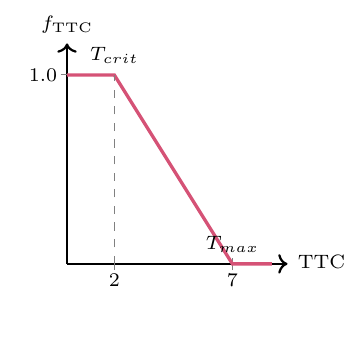
\begin{tikzpicture}
  \useasboundingbox (-0.5,-0.8) rectangle (3.2,3.0);
  \draw[->, thick] (0,0) -- (2.8,0) node[right,font=\scriptsize] {TTC (s)};
  \draw[->, thick] (0,0) -- (0,2.8) node[above,font=\scriptsize] {$f_{\text{TTC}}$};
  \node[font=\scriptsize, left] at (0,2.4) {1.0};
  \draw[gray, thin] (-0.08,2.4) -- (0.08,2.4);
  \node[font=\scriptsize, below] at (0.6,0) {2};
  \node[font=\scriptsize, below] at (2.1,0) {7};
  \draw[gray, thin] (0.6,-0.08) -- (0.6,0.08);
  \draw[gray, thin] (2.1,-0.08) -- (2.1,0.08);
  \draw[deeppink, very thick] (0,2.4) -- (0.6,2.4) -- (2.1,0) -- (2.6,0);
  \draw[gray, dashed, thin] (0.6,0) -- (0.6,2.4);
  \node[font=\scriptsize] at (0.6,2.65) {$T_{crit}$};
  \node[font=\scriptsize] at (2.1,0.25) {$T_{max}$};
\end{tikzpicture}%
}
\caption{碰撞时间因子}
\end{subfigure}
\hfill
\begin{subfigure}[b]{0.32\textwidth}
\centering
\resizebox{\textwidth}{!}{%
\begin{tikzpicture}
  \useasboundingbox (-0.5,-0.8) rectangle (3.2,3.0);
  \draw[->, thick] (0,0) -- (2.8,0) node[right,font=\scriptsize] {重叠率};
  \draw[->, thick] (0,0) -- (0,2.8) node[above,font=\scriptsize] {$f_{\text{ov}}$};
  \node[font=\scriptsize, left] at (0,2.4) {1.0};
  \draw[gray, thin] (-0.08,2.4) -- (0.08,2.4);
  \node[font=\scriptsize, below] at (2.4,0) {1.0};
  \node[font=\scriptsize, below] at (0,0) {0};
  \draw[deeppink, very thick] (0,0) -- (2.4,2.4);
\end{tikzpicture}%
}
\caption{横向重叠率因子}
\end{subfigure}
\hfill
\begin{subfigure}[b]{0.32\textwidth}
\centering
\resizebox{\textwidth}{!}{%
\begin{tikzpicture}
  \useasboundingbox (-0.5,-0.8) rectangle (3.2,3.0);
  % 内容居中: sigmoid 画在 [0.4, 2.8] 范围, 对称轴在 1.6
  \draw[->, thick] (0.2,0) -- (3.0,0) node[right,font=\scriptsize] {$v_{rel}/v_{max}$};
  \draw[->, thick] (0.2,0) -- (0.2,2.8) node[above,font=\scriptsize] {$f_{vel}$};
  \node[font=\scriptsize, left] at (0.2,2.4) {1.0};
  \draw[gray, thin] (0.12,2.4) -- (0.28,2.4);
  \node[font=\scriptsize, left] at (0.2,1.2) {0.5};
  \draw[gray, thin] (0.12,1.2) -- (0.28,1.2);
  % v_rel/v_max: -1 → x=0.4, 0 → x=1.6, 1 → x=2.8
  \draw[deeppink, very thick]
    plot[smooth, domain=0.4:2.8, samples=50] (\x, {2.4/(1+exp(-5*(\x-1.6)/1.2))});
  \node[font=\scriptsize, below] at (0.4,0) {$-1$};
  \node[font=\scriptsize, below] at (1.6,0) {$0$};
  \node[font=\scriptsize, below] at (2.8,0) {$1$};
  \draw[gray, dashed, thin] (1.6,0) -- (1.6,1.2);
\end{tikzpicture}%
}
\caption{相对速度因子}
\end{subfigure}

\vspace{0.8cm}

\hfill
\begin{subfigure}[b]{0.32\textwidth}
\centering
\resizebox{\textwidth}{!}{%
\begin{tikzpicture}
  \useasboundingbox (-0.5,-0.8) rectangle (3.2,3.0);
  \draw[->, thick] (0,0) -- (2.8,0);
  \draw[->, thick] (0,0) -- (0,2.8) node[above,font=\scriptsize] {$f_{\text{type}}$};
  \node[font=\scriptsize, left] at (0,2.4) {1.0};
  \draw[gray, thin] (-0.08,2.4) -- (0.08,2.4);
  \node[font=\scriptsize, left] at (0,1.68) {0.7};
  \draw[gray, thin] (-0.08,1.68) -- (0.08,1.68);
  \node[font=\scriptsize, left] at (0,0.72) {0.3};
  \draw[gray, thin] (-0.08,0.72) -- (0.08,0.72);
  \fill[dangerred!60] (0.2,0) rectangle (0.7,2.4);
  \fill[lightorange!80] (0.9,0) rectangle (1.4,1.68);
  \fill[deepblue!40] (1.6,0) rectangle (2.1,0.72);
  \node[font=\scriptsize] at (0.45,-0.35) {行人};
  \node[font=\scriptsize] at (1.15,-0.35) {车辆};
  \node[font=\scriptsize] at (1.85,-0.35) {静态};
\end{tikzpicture}%
}
\caption{障碍物类型因子}
\end{subfigure}
\hspace{0.02\textwidth}
\begin{subfigure}[b]{0.32\textwidth}
\centering
\resizebox{\textwidth}{!}{%
\begin{tikzpicture}
  \useasboundingbox (-0.5,-0.8) rectangle (3.2,3.0);
  \draw[->, thick] (0,0) -- (2.8,0) node[right,font=\scriptsize] {$d_{ij}$ (m)};
  \draw[->, thick] (0,0) -- (0,2.8) node[above,font=\scriptsize] {贡献};
  \node[font=\scriptsize, left] at (0,2.4) {1.0};
  \draw[gray, thin] (-0.08,2.4) -- (0.08,2.4);
  \node[font=\scriptsize, below] at (2.4,0) {$d_{cl}{=}10$};
  \draw[gray, thin] (2.4,-0.08) -- (2.4,0.08);
  \draw[deeppink, very thick] (0,2.4) -- (2.4,0) -- (2.7,0);
  \node[font=\scriptsize, deeppink] at (1.6,2.0) {$\frac{d_{cl}-d_{ij}}{d_{cl}}$};
\end{tikzpicture}%
}
\caption{单邻居交互贡献}
\end{subfigure}
\hfill

\end{figure}
\vspace*{\fill}
\clearpage

% ============================================================
% 算法总流程
% ============================================================
\vspace*{\fill}
\begin{center}% MIKU 多障碍物统一规划算法总流程
\begin{tikzpicture}[
    scale=1.0, transform shape,
    stepimp/.style={rectangle, rounded corners=3pt, draw=deeppink, fill=improvedpink, minimum width=5.4cm, minimum height=1.0cm, font=\small, align=center},
    inp/.style={rectangle, draw=deepblue, fill=inputyellow, minimum width=4.0cm, minimum height=0.8cm, font=\footnotesize, align=center},
    outnode/.style={rectangle, rounded corners=3pt, draw=deeppink, fill=outputpink, minimum width=4.0cm, minimum height=0.8cm, font=\small\bfseries, align=center},
    qpnode/.style={rectangle, rounded corners=3pt, draw=deepblue, fill=lightblue, minimum width=4.0cm, minimum height=0.8cm, font=\small\bfseries, align=center},
    arr/.style={-Stealth, thick, deepblue},
    injarr/.style={-Stealth, thick, deeppink},
]

% 输入
\node[inp] (i1) at (-5.8, 6.0) {参考线 $+$ 障碍物集合};
\node[inp] (i2) at (-5.8, 5.0) {预测轨迹 $+$ 车辆状态};

% 步骤（间距 1.7，全部为 MIKU 改进）
\node[stepimp] (s1) at (0, 5.5)  {\textbf{Step 1} 到达时间 $\tau(s)$ 与时变 SL 投影};
\node[stepimp] (s2) at (0, 3.8)  {\textbf{Step 2} 多因子威胁度评估 $\Theta_i$};
\node[stepimp] (s3) at (0, 2.1)  {\textbf{Step 3} 动态安全裕度 $\delta_i$ 与边界 $u_i,v_i$};
\node[stepimp] (s4) at (0, 0.4)  {\textbf{Step 4} 扫描线重叠分组 $\mathcal{G}_1,\ldots,\mathcal{G}_m$};
\node[stepimp] (s5) at (0,-1.3)  {\textbf{Step 5} 组内最大间隙 $g^\star_j=\max_k g_{j,k}$};
\node[stepimp] (s6) at (0,-3.0)  {\textbf{Step 6} 合并全局路径横向边界};
\node[stepimp] (s7) at (0,-4.7)  {\textbf{Step 7} ST 时空可通行走廊 $\Omega$};

% 输出（左侧）与跨接口的速度 QP
\node[outnode] (o1) at (-5.8,-3.0) {路径横向边界};
\node[outnode] (o2) at (-5.8,-4.7) {时空可通行走廊};
\node[qpnode]  (qp) at (-5.8,-6.4) {速度 QP（求解器不变）};

% 输入箭头
\draw[arr] (i1.east) -- (s1.west);
\draw[arr] (i2.east) -- (s1.west);

% 步骤间箭头
\draw[arr] (s1) -- (s2);
\draw[arr] (s2) -- (s3);
\draw[arr] (s3) -- (s4);
\draw[arr] (s4) -- (s5);
\draw[arr] (s5) -- (s6);
\draw[arr] (s6) -- (s7);

% 输出箭头
\draw[arr] (s6.west) -- (o1.east);
\draw[arr] (s7.west) -- (o2.east);

% 走廊注入速度 QP（跨解耦接口）
\draw[injarr] (o2.south) -- node[right, font=\footnotesize, deeppink] {逐时间步纵向上界} (qp.north);

\end{tikzpicture}
\end{center}
\vspace*{\fill}
\clearpage

% ============================================================
% 计算开销分解
% ============================================================
\vspace*{\fill}
\begin{center}% 改进算法各组件耗时分布
\begin{tikzpicture}[scale=1.0, transform shape]

% === 左：堆叠条形图（组件耗时绝对值）===
\begin{scope}[shift={(0,0)}]
  \draw[->, thick] (0,0) -- (10.5,0) node[right,font=\scriptsize] {耗时 (ms)};
  \draw[->, thick] (0,-0.3) -- (0,4.2) node[above,font=\scriptsize] {障碍物数 $n$};

  % Y 轴刻度
  \foreach \n/\y in {5/0.5, 10/1.5, 20/2.5, 40/3.5} {
    \draw[thick] (-0.1,\y) -- (0,\y);
    \node[font=\scriptsize, left] at (-0.1,\y) {$n=\n$};
  }

  % n=5, 总计 ≈ 3.2ms
  \fill[deeppink] (0,0.3) rectangle (0.8,0.7);
  \fill[improvedpink] (0.8,0.3) rectangle (1.4,0.7);
  \fill[deepblue] (1.4,0.3) rectangle (2.0,0.7);
  \fill[lightblue] (2.0,0.3) rectangle (3.0,0.7);
  \fill[skyblue] (3.0,0.3) rectangle (3.6,0.7);
  \node[font=\scriptsize, right] at (3.7,0.5) {3.2 ms};

  % n=10, 总计 ≈ 5.0ms
  \fill[deeppink] (0,1.3) rectangle (1.1,1.7);
  \fill[improvedpink] (1.1,1.3) rectangle (2.0,1.7);
  \fill[deepblue] (2.0,1.3) rectangle (2.8,1.7);
  \fill[lightblue] (2.8,1.3) rectangle (4.1,1.7);
  \fill[skyblue] (4.1,1.3) rectangle (5.0,1.7);
  \node[font=\scriptsize, right] at (5.1,1.5) {5.0 ms};

  % n=20, 总计 ≈ 8.5ms
  \fill[deeppink] (0,2.3) rectangle (1.6,2.7);
  \fill[improvedpink] (1.6,2.3) rectangle (3.0,2.7);
  \fill[deepblue] (3.0,2.3) rectangle (4.2,2.7);
  \fill[lightblue] (4.2,2.3) rectangle (6.8,2.7);
  \fill[skyblue] (6.8,2.3) rectangle (8.5,2.7);
  \node[font=\scriptsize, right] at (8.6,2.5) {8.5 ms};

  % n=40, 总计 ≈ 15.2ms
  \fill[deeppink] (0,3.3) rectangle (2.4,3.7);
  \fill[improvedpink] (2.4,3.3) rectangle (4.6,3.7);
  \fill[deepblue] (4.6,3.3) rectangle (6.4,3.7);
  \fill[lightblue] (6.4,3.3) rectangle (11.0,3.7);
  \fill[skyblue] (11.0,3.3) rectangle (13.8,3.7);
  \node[font=\scriptsize, right] at (13.9,3.5) {15.2 ms};

  % 实时性参考线 20ms
  \draw[dangerred, very thick, dashed] (13.8,-0.1) -- (13.8,4.0);
  \node[dangerred, font=\scriptsize, rotate=90, anchor=south] at (14.0,2) {实时阈值 20 ms};


\end{scope}

% === 图例 ===
\begin{scope}[shift={(0,-1.0)}]
  \fill[deeppink] (0,0) rectangle (0.4,0.3);
  \node[font=\footnotesize, anchor=west] at (0.5,0.15) {扫描线分组};
  \fill[improvedpink] (3.0,0) rectangle (3.4,0.3);
  \node[font=\footnotesize, anchor=west] at (3.5,0.15) {时变投影};
  \fill[deepblue] (5.8,0) rectangle (6.2,0.3);
  \node[font=\footnotesize, anchor=west] at (6.3,0.15) {路径边界合并};
  \fill[lightblue] (9.2,0) rectangle (9.6,0.3);
  \node[font=\footnotesize, anchor=west] at (9.7,0.15) {DP 速度搜索};
  \fill[skyblue] (12.5,0) rectangle (12.9,0.3);
  \node[font=\footnotesize, anchor=west] at (13.0,0.15) {QP 速度优化};
\end{scope}

\end{tikzpicture}
\end{center}
\vspace*{\fill}
\clearpage

% ============================================================
% 贪心 vs 全局协调 子图a
% ============================================================
\vspace*{\fill}\begin{center}% 贪心独立决策 → BLOCKED（子图 a）
\begin{tikzpicture}[scale=0.85, transform shape]
  % 道路
  \fill[bglight] (-0.5,-2.5) rectangle (8.5,2.5);
  \draw[gray, thick] (-0.5, 2.5) -- (8.5, 2.5);
  \draw[gray, thick] (-0.5,-2.5) -- (8.5,-2.5);
  \draw[dashed, gray!60] (-0.5, 0) -- (8.5, 0);
  \node[gray, font=\scriptsize, anchor=east] at (-0.6, 0) {$l{=}0$};

  % O_a（上方靠边）y=[0.5, 1.0]
  \fill[dangerred!70, draw=dangerred, thick] (3.2, 0.5) rectangle (4.8, 1.0);
  \node[font=\scriptsize, white] at (4.0, 0.75) {$O_a$};

  % O_b（下方靠边）y=[-1.0, -0.5]
  \fill[dangerred!70, draw=dangerred, thick] (3.2,-1.0) rectangle (4.8,-0.5);
  \node[font=\scriptsize, white] at (4.0,-0.75) {$O_b$};

  % 膨胀虚线 δ=0.4
  \draw[dangerred!60, dashed, thick] (2.8, 0.1) rectangle (5.2, 1.4);
  \draw[dangerred!60, dashed, thick] (2.8,-1.4) rectangle (5.2,-0.1);

  % 决策标注
  \node[deepblue, font=\scriptsize\bfseries] at (5.5, 0.75) {R};
  \node[deeppink, font=\scriptsize\bfseries] at (2.5,-0.75) {L};

  % 独立决策：O_a 右绕 → 上界压到 0.1-0.1=0.0
  %           O_b 左绕 → 下界抬到 -0.1+0.1=0.0
  % l+ ≈ l- → BLOCKED

  % 上界 l+(s) 凹字形（offset 区分）
  \draw[deeppink, very thick]
    (-0.5, 2.5) -- (2.6, 2.5) -- (2.6, 0.0) -- (5.4, 0.0) -- (5.4, 2.5) -- (8.5, 2.5);
  \node[deeppink, font=\scriptsize] at (7.5, 2.1) {$l^+(s)$};

  % 下界 l-(s) 凸字形
  \draw[deepblue, very thick]
    (-0.5,-2.5) -- (2.6,-2.5) -- (2.6, 0.0) -- (5.4, 0.0) -- (5.4,-2.5) -- (8.5,-2.5);
  \node[deepblue, font=\scriptsize] at (7.5,-2.1) {$l^-(s)$};

  % BLOCKED 标注
  \node[dangerred, font=\scriptsize\bfseries] at (4.0, 1.8) {$l^+ \leq l^-$ $\Rightarrow$ BLOCKED};

  % 自车
  \fill[deepblue, opacity=0.4] (0.3,-0.3) rectangle (1.8,0.3);
  \draw[deepblue, thick, rounded corners=1pt] (0.3,-0.3) rectangle (1.8,0.3);
  \node[deepblue, font=\tiny\bfseries] at (1.05,0) {自车};
\end{tikzpicture}
\end{center}\vspace*{\fill}\clearpage
% ============================================================
% 贪心 vs 全局协调 子图b
% ============================================================
\vspace*{\fill}\begin{center}% 全局协调统一右绕 → 通行（子图 b）
\begin{tikzpicture}[scale=0.85, transform shape]
  % 道路
  \fill[bglight] (-0.5,-2.5) rectangle (8.5,2.5);
  \draw[gray, thick] (-0.5, 2.5) -- (8.5, 2.5);
  \draw[gray, thick] (-0.5,-2.5) -- (8.5,-2.5);
  \draw[dashed, gray!60] (-0.5, 0) -- (8.5, 0);
  \node[gray, font=\scriptsize, anchor=east] at (-0.6, 0) {$l{=}0$};

  % O_a（上方靠边）y=[0.5, 1.0]
  \fill[dangerred!70, draw=dangerred, thick] (3.2, 0.5) rectangle (4.8, 1.0);
  \node[font=\scriptsize, white] at (4.0, 0.75) {$O_a$};

  % O_b（下方靠边）y=[-1.0, -0.5]
  \fill[dangerred!70, draw=dangerred, thick] (3.2,-1.0) rectangle (4.8,-0.5);
  \node[font=\scriptsize, white] at (4.0,-0.75) {$O_b$};

  % 膨胀虚线 δ=0.4（统一右绕）
  \draw[dangerred!60, dashed, thick] (2.8, 0.1) rectangle (5.2, 1.4);
  \draw[dangerred!60, dashed, thick] (2.8,-1.4) rectangle (5.2,-0.1);

  % 决策标注（统一 R）
  \node[deepblue, font=\scriptsize\bfseries] at (5.5, 0.75) {R};
  \node[deepblue, font=\scriptsize\bfseries] at (5.5,-0.75) {R};

  % 统一右绕 → 上界压到 O_b 膨胀下缘 -1.4（offset -0.1）
  \draw[deeppink, very thick]
    (-0.5, 2.5) -- (2.6, 2.5) -- (2.6, -1.5) -- (5.4, -1.5) -- (5.4, 2.5) -- (8.5, 2.5);
  \node[deeppink, font=\scriptsize] at (7.5, 2.1) {$l^+(s)$};

  % 下界保持道路下界
  \draw[deepblue, very thick, dashed]
    (-0.5,-2.5) -- (8.5,-2.5);
  \node[deepblue, font=\scriptsize, left] at (-0.6,-2.5) {$l^-(s)$};

  % 通行带
  \fill[lightgreen, opacity=0.25] (-0.5,-2.5) rectangle (8.5,-1.5);

  % 通行带宽度
  \draw[lightgreen!60!black, thick, {Stealth}-{Stealth}] (0.5,-2.5) -- (0.5,-1.5);
  \node[lightgreen!60!black, font=\scriptsize, anchor=east] at (0.4,-2.0) {$W{=}1.0$m};

  % 自车轨迹（无 fill）
  \draw[deepblue, very thick, -{Stealth}]
    plot[smooth, tension=0.55] coordinates
      {(0.5, 0) (1.5,-0.5) (2.5,-1.8) (4.0,-2.0) (5.5,-1.8) (6.5,-0.5) (7.5, 0)};
  \node[deepblue, font=\scriptsize] at (4.0,-2.4) {规划轨迹};

  % PASS 判定
  \node[draw=lightgreen!80!black, fill=lightgreen!20, font=\scriptsize,
        rounded corners=3pt] at (4.0, 2.0)
    {统一右绕 $\Rightarrow$ \textbf{PASS}};
\end{tikzpicture}
\end{center}\vspace*{\fill}\clearpage

% ============================================================
% 扫描线分组过程
% ============================================================
\vspace*{\fill}
\begin{center}% 扫描线按 s_i^- 升序合并连通分量的过程
\begin{tikzpicture}[scale=0.95, transform shape,
    obs/.style={fill=dangerred!70, draw=dangerred, thick, rounded corners=1pt},
    grp/.style={draw=deeppink, very thick, dashed, rounded corners=3pt},
]

% s 轴
\draw[-Stealth, thick] (0,0) -- (14.5,0) node[right, font=\small] {$s$};
\foreach \x/\lab in {0/0, 2/10, 4/20, 6/30, 8/40, 10/50, 12/60, 14/70}
    \draw[thick] (\x,-0.1) -- (\x,0.1) node[below=0.1cm, font=\scriptsize] {\lab};

% 六个障碍物的 [s^-, s^+] 区间（按 s^- 升序）
% O1: [5, 15]  O2: [10, 22]  O3: [30, 38]  O4: [34, 44]  O5: [42, 50]  O6: [60, 68]
\fill[obs] (1,0.6) rectangle (3,1.1);
\node[white, font=\scriptsize\bfseries] at (2,0.85) {$O_1$};

\fill[obs] (2,1.4) rectangle (4.4,1.9);
\node[white, font=\scriptsize\bfseries] at (3.2,1.65) {$O_2$};

\fill[obs] (6,0.6) rectangle (7.6,1.1);
\node[white, font=\scriptsize\bfseries] at (6.8,0.85) {$O_3$};

\fill[obs] (6.8,1.4) rectangle (8.8,1.9);
\node[white, font=\scriptsize\bfseries] at (7.8,1.65) {$O_4$};

\fill[obs] (8.4,0.6) rectangle (10,1.1);
\node[white, font=\scriptsize\bfseries] at (9.2,0.85) {$O_5$};

\fill[obs] (12,0.6) rectangle (13.6,1.1);
\node[white, font=\scriptsize\bfseries] at (12.8,0.85) {$O_6$};

% s_max 扫描线（当前最大上界）
\draw[deepblue, very thick, densely dotted] (4.4,-0.3) -- (4.4,3.0);
\node[deepblue, font=\scriptsize, anchor=south] at (4.4,3.0) {$s_{\max}=22$};

\draw[deepblue, very thick, densely dotted] (10,-0.3) -- (10,3.0);
\node[deepblue, font=\scriptsize, anchor=south] at (10,3.0) {$s_{\max}=50$};

\draw[deepblue, very thick, densely dotted] (13.6,-0.3) -- (13.6,3.0);
\node[deepblue, font=\scriptsize, anchor=south] at (13.6,3.0) {$s_{\max}=68$};

% 三个连通分量分组框
\draw[grp] (0.7,0.4) rectangle (4.7,2.1);
\node[deeppink, font=\small\bfseries, anchor=south] at (2.7,2.1) {$C_1=\{O_1,O_2\}$};
\node[deeppink!80, font=\scriptsize, anchor=north west] at (0.78,0.43) {$s_{\min}{=}5$};

\draw[grp] (5.7,0.4) rectangle (10.3,2.1);
\node[deeppink, font=\small\bfseries, anchor=south] at (8,2.1) {$C_2=\{O_3,O_4,O_5\}$};
\node[deeppink!80, font=\scriptsize, anchor=north west] at (5.78,0.43) {$s_{\min}{=}30$};

\draw[grp] (11.7,0.4) rectangle (13.9,2.1);
\node[deeppink, font=\small\bfseries, anchor=south] at (12.8,2.1) {$C_3=\{O_6\}$};
\node[deeppink!80, font=\scriptsize, anchor=north west] at (11.78,0.43) {$s_{\min}{=}60$};

\end{tikzpicture}
\end{center}
\vspace*{\fill}
\clearpage

% ============================================================
% 到达时间估计对比
% ============================================================
\vspace*{\fill}
\begin{center}% 到达时间估计：匀速 vs 二阶运动学
\begin{tikzpicture}
\begin{axis}[
    width=11cm, height=7cm,
    xlabel={$s - s_{ego}$ \;(m)}, ylabel={$\tau(s)$ \;(s)},
    xmin=0, xmax=30, ymin=0, ymax=6,
    grid=both, grid style={gray!25},
    legend style={at={(0.02,0.98)}, anchor=north west, font=\small, draw=deepblue},
    axis line style={thick},
    tick label style={font=\footnotesize},
    label style={font=\small},
]

% 匀速假设 tau_0 = s/v_ego, v_ego=5
\addplot[deepblue, very thick, samples=50, domain=0:30] {x/5};
\addlegendentry{$\tau_0(s)=s/v_{ego}$ 匀速假设}

% 二阶模型 tau = (-v + sqrt(v^2 + 2 a s))/a, v=5, a=2
\addplot[deeppink, very thick, samples=80, domain=0:30] {(-5 + sqrt(25 + 4*x))/2};
\addlegendentry{$\tau(s)$ 二阶运动学}

% 原始速度曲线反推: v(t)=5+2(1-e^{-t}), s(t)=7t-2+2 e^{-t}
% 取参数 t 等距采样得 (s, tau) 对
\addplot[lightgreen!55!black, very thick, densely dashed] coordinates {
  (0, 0) (2.71, 0.5) (5.74, 1.0) (8.95, 1.5) (12.27, 2.0)
  (15.66, 2.5) (19.10, 3.0) (22.56, 3.5) (26.04, 4.0) (29.52, 4.5)
};
\addlegendentry{$\tau_{\mathrm{true}}(s)$ 原始速度曲线反推}

% 误差标注（在 s=20 处）
% tau0(20) = 20/5 = 4.0
% tau(20)  = (-5 + sqrt(25 + 4*20))/2 = (-5 + sqrt(105))/2 ≈ 2.62
% tau_true(20) ≈ 3.13（绿色采样点线性插值）
\draw[dangerred, thick, densely dashed] (axis cs:20,0) -- (axis cs:20,4);

% 匀速误差 = 4.00 - 3.13 = 0.87 s
\draw[<->, thick, dangerred] (axis cs:20,3.13) -- (axis cs:20,4);
\node[dangerred, font=\footnotesize, anchor=west] at (axis cs:20.3,3.56) {匀速误差 ${\approx}\,0.87$ s};

% 二阶残差 = 3.13 - 2.62 = 0.51 s
\draw[<->, thick, lightorange!80!black] (axis cs:20,2.62) -- (axis cs:20,3.13);
\node[lightorange!80!black, font=\footnotesize, anchor=west] at (axis cs:20.3,2.88) {二阶残差 ${\approx}\,0.51$ s};

% 关键点
\addplot[deepblue, mark=*, mark size=2pt, only marks] coordinates {(20,4)};
\addplot[lightgreen!55!black, mark=*, mark size=2pt, only marks] coordinates {(20,3.13)};
\addplot[deeppink, mark=*, mark size=2pt, only marks] coordinates {(20,2.62)};

\node[deepblue, font=\scriptsize, anchor=south] at (axis cs:20,4.08) {$\tau_0{=}4.00$};
\node[deeppink, font=\scriptsize, anchor=north] at (axis cs:20,2.54) {$\tau{=}2.62$};

% 参数标注
\node[rectangle, draw=deepblue, fill=bglight, rounded corners=3pt, font=\footnotesize, align=left] at (axis cs:22,1) {$v_{ego}=5$ m/s\\$a_{ego}=2$ m/s$^2$};

\end{axis}
\end{tikzpicture}
\end{center}
\vspace*{\fill}
\clearpage

% ============================================================
% 时变 SL 投影 pipeline
% ============================================================
\vspace*{\fill}
\begin{center}% 动态障碍物时变SL投影 pipeline
\begin{tikzpicture}[scale=0.92, transform shape,
    stage/.style={rectangle, rounded corners=3pt, draw=deeppink, fill=improvedpink, minimum width=3.3cm, minimum height=1.35cm, font=\small, align=center},
    data/.style={rectangle, draw=deepblue, fill=inputyellow, minimum width=3.0cm, minimum height=0.9cm, font=\footnotesize, align=center},
    outbox/.style={rectangle, rounded corners=3pt, draw=deeppink, fill=outputpink, minimum width=3.2cm, minimum height=1.1cm, font=\small\bfseries, align=center},
    arr/.style={-Stealth, thick, deepblue},
    tauarr/.style={-Stealth, thick, dashed, deeppink},
    midlab/.style={font=\scriptsize, deepblue, inner sep=1pt},
]

% 主流水线：水平四步
\node[stage] (s1) at (0,0) {\textbf{Step 1}\\轨迹查询\\(线性插值)};
\node[stage] (s2) at (4.1,0) {\textbf{Step 2}\\Cartesian 到\\ Frenet 投影};
\node[stage] (s3) at (8.2,0) {\textbf{Step 3}\\时变 SL 边界\\$[l_i^-(\tau),l_i^+(\tau)]$};
\node[stage] (s4) at (12.3,0) {\textbf{Step 4}\\活跃性过滤\\(距离阈值)};

% 主流水线箭头 + 中间态标签（贴在箭头上方，白底）
\draw[arr] (s1) -- node[midlab, above=1pt] {$(x_i(\tau),y_i(\tau))$} (s2);
\draw[arr] (s2) -- node[midlab, above=1pt] {$(s_i(\tau),l_i(\tau))$} (s3);
\draw[arr] (s3) -- node[midlab, above=1pt] {$u_i(\tau),v_i(\tau)$} (s4);

% 输入：从左侧水平流入 Step 1
\node[data] (in) at (-4.2,0) {Prediction 轨迹\\$\{(x_i(t_j),y_i(t_j))\}$};
\draw[arr] (in) -- (s1);

% 输出：从 Step 4 水平流出
\node[outbox] (out) at (16.3,0) {活跃障碍物集\\ $+$ 时变 $u_i,v_i$};
\draw[arr] (s4) -- (out);

% 自车到达时间 tau(s)：上方横向总线，正交注入 Step1/2/3 顶部
\node[data, fill=improvedpink, draw=deeppink] (tau) at (-4.2,2.4) {自车到达时间 $\tau(s)$};

% 横向总线：从 tau 延伸到 s3 上方
\coordinate (busL) at (tau.east);
\coordinate (busR) at (s3.north |- 0,2.4);
\draw[tauarr, -] (busL) -- (busR);

% 三条向下的短虚线，分别接入 Step1/2/3 顶部
\draw[tauarr] (s1.north |- 0,2.4) -- (s1.north);
\draw[tauarr] (s2.north |- 0,2.4) -- (s2.north);
\draw[tauarr] (s3.north |- 0,2.4) -- (s3.north);

% 总线标签
\node[font=\scriptsize, deeppink, anchor=south] at ($(s1.north |- 0,2.4)!0.5!(s2.north |- 0,2.4)$) {参数注入 $\tau$};

\end{tikzpicture}
\end{center}
\vspace*{\fill}
\clearpage

% ============================================================
% Baseline 贪心流程
% ============================================================
\vspace*{\fill}
\begin{center}% Apollo Baseline 贪心策略流程
\begin{tikzpicture}[scale=0.95, transform shape,
    box/.style={rectangle, rounded corners=3pt, draw=deepblue, fill=lightblue, minimum width=5.0cm, minimum height=0.9cm, font=\small, align=center},
    dec/.style={diamond, draw=deepblue, fill=inputyellow, aspect=2.2, inner sep=2pt, font=\small, align=center},
    bad/.style={rectangle, rounded corners=3pt, draw=dangerred, fill=dangerred!25, minimum width=4.2cm, minimum height=0.9cm, font=\small, align=center},
    arr/.style={-Stealth, thick, deepblue},
    arrbad/.style={-Stealth, thick, dangerred},
]

\node[box] (init) at (0,8.4) {初始化 $l^{\pm}(s)=l^{\pm}_{road}(s)$};
\node[box] (loop) at (0,6.8) {遍历活跃障碍物 $O_i$};
\node[dec]  (side) at (0,4.8) {仅单侧可通行?};
\node[box] (greedy) at (5.5,4.8) {比较 $\frac{l_i^-+l_i^+}{2}$ 与 $l_{last\_nudge}$};
\node[box] (assign) at (0,2.8) {指派 $d_i \in \{L,R\}$，更新 $l^{\pm}$};
\node[dec]  (blk) at (0,0.8) {$l^+ < l^-$?};
\node[bad] (trim) at (5.5,0.8) {\texttt{TrimPathBounds} 截断};
\node[bad] (fb) at (5.5,-0.8) {FallbackPath 停车};
\node[box] (more) at (0,-0.8) {下一个 $O_i$};
\node[rectangle, rounded corners=3pt, draw=deeppink, fill=outputpink, minimum width=5.0cm, minimum height=0.9cm, font=\small\bfseries, align=center] (out) at (0,-2.6) {输出 path\_boundary};

\draw[arr] (init) -- (loop);
\draw[arr] (loop) -- (side);
\draw[arr] (side.east) -- node[above, font=\scriptsize] {否} (greedy.west);
\draw[arr] (greedy.south) |- (assign.east);
\draw[arr] (side.south) -- node[right, font=\scriptsize] {是，直接赋可通侧} (assign.north);
\draw[arr] (assign) -- (blk);
\draw[arrbad] (blk.east) -- node[above, font=\scriptsize] {是} (trim.west);
\draw[arrbad] (trim) -- (fb);
\draw[arr] (blk.west) -| node[above left=0.05cm, font=\scriptsize] {否} ++(-2.5,0) |- (more.west);
\draw[arr] (more.west) -- ++(-2.5,0) |- (loop.west);
\draw[arr] (more) -- node[right, font=\scriptsize] {遍历结束} (out);

\end{tikzpicture}
\end{center}
\vspace*{\fill}
\clearpage

% ============================================================
% 三级降级状态转移
% ============================================================
\vspace*{\fill}
\begin{center}% 三级降级机制状态转移
\begin{tikzpicture}[scale=0.95, transform shape,
    level/.style={rectangle, rounded corners=4pt, draw=#1, line width=1.2pt,
        fill=#1!12, minimum width=15.4cm, minimum height=2.2cm},
    badge/.style={circle, draw=#1, fill=#1, text=white, font=\small\bfseries,
        minimum size=0.7cm, inner sep=0pt},
    trigbox/.style={rectangle, rounded corners=3pt, draw=dangerred, fill=dangerred!15,
        minimum width=5.0cm, minimum height=0.9cm, font=\small, align=center},
    actbox/.style={rectangle, rounded corners=3pt, draw=deepblue, fill=lightblue,
        minimum width=5.0cm, minimum height=0.9cm, font=\small, align=center},
    arr/.style={-Stealth, thick, deepblue},
    arrdanger/.style={-Stealth, thick, dangerred},
    arrback/.style={-Stealth, thick, deeppink, densely dashed},
    conn/.style={-Stealth, very thick, gray!80},
]

% 主流程入口
\node[rectangle, rounded corners=4pt, draw=deeppink, line width=1.2pt,
    fill=improvedpink, minimum width=6cm, minimum height=1cm,
    font=\normalsize\bfseries] (main) at (0,0) {改进算法主流程};

% L3（最轻）
\node[level=deepblue] (l3bg) at (0,-2.4) {};
\node[badge=deepblue] at (-7.0,-1.7) {L3};
\node[font=\small\bfseries, deepblue, anchor=west] at (-6.4,-1.7) {轻度降级};
\node[font=\scriptsize, gray, anchor=east] at (7.3,-1.7) {实测频率 $<$1\%};
\node[trigbox] (t3) at (-3.0,-2.7) {分组内 $k>k_{\max}$（感知误检或极端拥堵）};
\node[actbox] (a3) at (4.0,-2.7) {组内回退Baseline逐障碍贪心};
\draw[conn] (t3) -- (a3);

% L2（中等）
\node[level=lightorange] (l2bg) at (0,-5.2) {};
\node[badge=lightorange] at (-7.0,-4.5) {L2};
\node[font=\small\bfseries, lightorange, anchor=west] at (-6.4,-4.5) {中度降级};
\node[font=\scriptsize, gray, anchor=east] at (7.3,-4.5) {实测频率 $<$1\%};
\node[trigbox] (t2) at (-3.0,-5.5) {预测轨迹缺失或超出时间范围};
\node[actbox] (a2) at (4.0,-5.5) {障碍物退化为静态，使用$t{=}0$快照};
\draw[conn] (t2) -- (a2);

% L1（最严重）
\node[level=dangerred] (l1bg) at (0,-8.0) {};
\node[badge=dangerred] at (-7.0,-7.3) {L1};
\node[font=\small\bfseries, dangerred, anchor=west] at (-6.4,-7.3) {重度降级};
\node[font=\scriptsize, gray, anchor=east] at (7.3,-7.3) {实测频率 3--5\%};
\node[trigbox] (t1) at (-3.0,-8.3) {$W^* \leq 0$，所有间隙不足车宽};
\node[actbox] (a1) at (4.0,-8.3) {\texttt{TrimPathBounds} + FallbackPath停车};
\draw[conn] (t1) -- (a1);

% 主流程 → 三级
\draw[arrdanger] (main.south) -- (l3bg.north);
\draw[arrdanger] (l3bg.south) -- (l2bg.north);
\draw[arrdanger] (l2bg.south) -- (l1bg.north);

% 恢复箭头
\draw[arrback] (a3.east) -- ++(0.8,0) |- node[pos=0.25, right, font=\scriptsize, deeppink] {恢复} (main.east);
\draw[arrback] (a2.east) -- ++(1.6,0) |- (main.east);

\end{tikzpicture}
\end{center}
\vspace*{\fill}
\clearpage

% ============================================================
% 路径-速度信息断层
% ============================================================
\vspace*{\fill}
\begin{center}% 路径与速度规划之间的单向信息传递与时空约束缺口
\begin{tikzpicture}[scale=0.95, transform shape,
    infobox/.style={rectangle, rounded corners=4pt, draw=deepblue, fill=lightblue!30,
        minimum width=3.8cm, align=left, font=\small, inner sep=8pt},
    recvbox/.style={rectangle, rounded corners=4pt, draw=deepblue, fill=bglight,
        minimum width=3.8cm, align=left, font=\small, inner sep=8pt},
    lostitem/.style={rectangle, rounded corners=2pt, draw=dangerred!70, fill=dangerred!8,
        font=\small, inner sep=4pt},
]

% ===== Left: Path 阶段产生的决策信息 =====
\node[infobox, minimum height=3.8cm] (pathbox) at (0, 0) {%
    \textbf{Path 阶段产生的决策信息}\\[5pt]
    \textcolor{deepblue}{\textbullet}~避让方向 $d_i$\\[3pt]
    \textcolor{deepblue}{\textbullet}~横向边界 $[l^-(s),\,l^+(s)]$\\[3pt]
    \textcolor{deepblue}{\textbullet}~时间前提 $t_{\mathrm{clear}}$\\[3pt]
    \textcolor{deepblue}{\textbullet}~威胁度评估 $\theta_i$%
};

% ===== Right: Speed 阶段接收的信息 =====
\node[recvbox, minimum height=3.0cm] (speedbox) at (11.5, 0) {%
    \textbf{Speed 阶段接收的信息}\\[5pt]
    \textcolor{deepblue}{\textbullet}\;$[l^-(s),\,l^+(s)]$\\[1pt]
    {\footnotesize\textcolor{deepblue}{知道路径在哪里}}\\[6pt]
    \textcolor{dangerred}{\texttimes}\;$d_i,\;t_{\mathrm{clear}},\;\theta_i$\\[1pt]
    {\footnotesize\textcolor{dangerred}{不知道路径为什么在那里}}%
};

% ===== Middle: 传递瓶颈（漏斗形，内部干净） =====
\coordinate (fTL) at (4.6, 1.9);
\coordinate (fBL) at (4.6,-1.9);
\coordinate (fTR) at (7.8, 0.55);
\coordinate (fBR) at (7.8,-0.55);

\fill[bglight, draw=deepblue!60, thick]
    (fTL) -- (fTR) -- (fBR) -- (fBL) -- cycle;

\node[font=\small\bfseries, deepblue!80] at (6.1, 2.3) {传递瓶颈};

% 一根蓝色箭头从 pathbox 穿过漏斗到 speedbox
\draw[deepblue, very thick, -Stealth] (pathbox.east) -- (speedbox.west)
    node[midway, above, font=\small\bfseries, deepblue] {$[l^-(s),\,l^+(s)]$};

% ===== 丢失的信息：漏斗上下方标注，箭头撞向漏斗壁 =====
% 上方
\node[lostitem] (ld) at (5.0, 3.2) {$d_i$\;避让方向};
\node[lostitem] (lt) at (8.0, 3.2) {$t_{\mathrm{clear}}$\;时间前提};
\draw[dangerred, thick, -|] (ld.south) -- ($(fTL)!0.2!(fTR)$)
    node[pos=0.4, right, font=\small\bfseries, dangerred] {\texttimes};
\draw[dangerred, thick, -|] (lt.south) -- ($(fTL)!0.7!(fTR)$)
    node[pos=0.4, right, font=\small\bfseries, dangerred] {\texttimes};

% 下方
\node[lostitem] (lth) at (6.3, -3.2) {$\theta_i$\;威胁度评估};
\draw[dangerred, thick, -|] (lth.north) -- ($(fBL)!0.4!(fBR)$)
    node[pos=0.4, right, font=\small\bfseries, dangerred] {\texttimes};

\end{tikzpicture}
\end{center}
\vspace*{\fill}
\clearpage

% ============================================================
% 场景1轨迹 baseline
% ============================================================
\vspace*{\fill}\begin{center}% 场景一 S1-C 原始算法轨迹（子图 a）
\begin{tikzpicture}[scale=0.85, transform shape]
  \fill[bglight] (0,-1.5) rectangle (12,1.5);
  \draw[deepblue, very thick] (0,-1.5) -- (12,-1.5);
  \draw[deepblue, very thick] (0, 1.5) -- (12, 1.5);
  \draw[deepblue, dashed, thin] (0,0) -- (12,0);

  \fill[obsstatic] (2.2,-0.2) rectangle (2.7,0.35);
  \fill[obsstatic] (4.0,-0.35) rectangle (4.5,0.2);
  \fill[obsstatic] (5.8,-0.1) rectangle (6.3,0.45);
  \fill[obsstatic] (7.6,-0.4) rectangle (8.1,0.15);
  \fill[obsstatic] (9.4,-0.2) rectangle (9.9,0.35);

  \draw[deepblue, very thick]
    plot[smooth, tension=0.5] coordinates {(0.3,0.1) (1.5,0.4) (2.9,0.7) (4.1,-0.7) (5.5,0.7) (6.5,0.1)};
  \fill[dangerred] (6.5,0.1) circle (4pt);
  \node[dangerred, font=\scriptsize\bfseries, anchor=south] at (6.5,0.25) {STOP};
  \draw[dangerred, ultra thick] (6.2,-0.2) -- (6.8,0.4);
  \draw[dangerred, ultra thick] (6.2,0.4) -- (6.8,-0.2);

  \fill[egopt] (0.3,-0.2) rectangle (0.9,0.2);
\end{tikzpicture}
\end{center}\vspace*{\fill}\clearpage
% ============================================================
% 场景1轨迹 改进
% ============================================================
\vspace*{\fill}\begin{center}% 场景一 S1-C 改进算法轨迹（子图 b）
\begin{tikzpicture}[scale=0.85, transform shape]
  \fill[bglight] (0,-1.5) rectangle (12,1.5);
  \draw[deepblue, very thick] (0,-1.5) -- (12,-1.5);
  \draw[deepblue, very thick] (0, 1.5) -- (12, 1.5);
  \draw[deepblue, dashed, thin] (0,0) -- (12,0);

  \fill[obsstatic] (2.2,-0.2) rectangle (2.7,0.35);
  \fill[obsstatic] (4.0,-0.35) rectangle (4.5,0.2);
  \fill[obsstatic] (5.8,-0.1) rectangle (6.3,0.45);
  \fill[obsstatic] (7.6,-0.4) rectangle (8.1,0.15);
  \fill[obsstatic] (9.4,-0.2) rectangle (9.9,0.35);

  \fill[lightgreen!30] (0,-1.0) rectangle (12,-0.7);
  \draw[deeppink, very thick]
    plot[smooth, tension=0.5] coordinates {(0.3,0) (1.5,-0.6) (3.0,-0.85) (4.5,-0.85) (6.0,-0.85) (7.5,-0.85) (9.0,-0.85) (10.5,-0.6) (11.7,-0.2)};

  \fill[egopt] (0.3,-0.2) rectangle (0.9,0.2);
  \fill[deeppink] (11.7,-0.2) circle (3pt);

  \node[lightgreen!40!black, font=\scriptsize, anchor=west] at (0.1,-0.85) {最优通行带};
\end{tikzpicture}
\end{center}\vspace*{\fill}\clearpage
% ============================================================
% 场景2轨迹 baseline
% ============================================================
\vspace*{\fill}\begin{center}% 场景二 S2-C 原始 BLOCKED（子图 a）
\begin{tikzpicture}[scale=0.85, transform shape]
  % 道路背景
  \begin{scope}[on background layer]
    \fill[bglight] (0,-1.5) rectangle (12,1.5);
  \end{scope}

  \draw[gray, thick] (0,-1.5) -- (12,-1.5);
  \draw[gray, thick] (0, 1.5) -- (12, 1.5);
  \draw[gray, dashed] (0,0) -- (12,0);

  % 障碍物（靠边）
  \fill[dangerred!70, draw=dangerred, thick] (4.5,0.6) rectangle (7.5,1.2);
  \node[font=\scriptsize, white] at (6.0,0.9) {$O_a$};
  \fill[dangerred!70, draw=dangerred, thick] (4.5,-1.2) rectangle (7.5,-0.6);
  \node[font=\scriptsize, white] at (6.0,-0.9) {$O_b$};

  % 矛盾避让区域标注（用半透明，放在 background layer 不遮挡）
  \begin{scope}[on background layer]
    \fill[deeppink!10] (4.5,-0.3) rectangle (7.5,1.2);
    \fill[deepblue!10] (4.5,-1.2) rectangle (7.5,0.3);
  \end{scope}

  % 自车
  \fill[deepblue, opacity=0.4] (0.3,-0.25) rectangle (1.5,0.25);
  \draw[deepblue, thick, rounded corners=1pt] (0.3,-0.25) rectangle (1.5,0.25);
  \node[deepblue, font=\tiny\bfseries] at (0.9,0) {自车};

  % 自车轨迹 → BLOCKED
  \draw[deepblue, very thick] (1.5,0) -- (3.8,0);
  \fill[dangerred] (3.8,0) circle (4pt);
  \draw[dangerred, ultra thick] (3.5,-0.3) -- (4.1,0.3);
  \draw[dangerred, ultra thick] (3.5,0.3) -- (4.1,-0.3);

  \node[dangerred, font=\scriptsize\bfseries] at (6.0,0) {$l^+ < l^-$};
  \node[dangerred, font=\scriptsize\bfseries, anchor=south] at (3.8,0.35) {BLOCKED};
\end{tikzpicture}
\end{center}\vspace*{\fill}\clearpage
% ============================================================
% 场景2轨迹 改进
% ============================================================
\vspace*{\fill}\begin{center}% 场景二 S2-C 改进中央通过（子图 b）
\begin{tikzpicture}[scale=0.85, transform shape]
  \fill[bglight] (0,-1.5) rectangle (12,1.5);
  \draw[deepblue, very thick] (0,-1.5) -- (12,-1.5);
  \draw[deepblue, very thick] (0, 1.5) -- (12, 1.5);
  \draw[deepblue, dashed, thin] (0,0) -- (12,0);

  \fill[obsstatic] (4.5,0.6) rectangle (7.5,1.2);
  \fill[obsstatic] (4.5,-1.2) rectangle (7.5,-0.6);

  \fill[lightgreen!30] (0,-0.35) rectangle (12,0.35);

  \draw[deeppink, very thick] (0.3,0) -- (11.7,0);

  \fill[egopt] (0.3,-0.2) rectangle (0.9,0.2);
  \fill[deeppink] (11.7,0) circle (3pt);

  \node[lightgreen!40!black, font=\scriptsize\bfseries, anchor=west] at (0.1,0.55) {最大中央间隙};
\end{tikzpicture}
\end{center}\vspace*{\fill}\clearpage
% ============================================================
% 场景3轨迹 baseline
% ============================================================
\vspace*{\fill}\begin{center}% 场景三 S3-C 原始 YIELD 停车（子图 a）
\begin{tikzpicture}[scale=0.85, transform shape]
  \fill[bglight] (0,-1.5) rectangle (12,1.5);
  \draw[deepblue, very thick] (0,-1.5) -- (12,-1.5);
  \draw[deepblue, very thick] (0, 1.5) -- (12, 1.5);
  \draw[deepblue, dashed, thin] (0,0) -- (12,0);

  \fill[obsstatic] (3.2,0.4) rectangle (3.8,1.0);
  \fill[obsstatic] (8.8,-1.0) rectangle (9.4,-0.4);
  \fill[obsdyn] (5.5,-0.5) rectangle (6.3,-0.1);
  \draw[-Stealth, thick, dangerred] (6.35,-0.3) -- (7.0,-0.3);
  \fill[obsdyn] (7.5,-0.2) rectangle (7.8,0.2);
  \draw[-Stealth, thick, dangerred] (7.65,0.25) -- (7.65,1.1);
  \node[dangerred, font=\scriptsize] at (7.65,1.3) {行人};

  \draw[deepblue, very thick] (0.3,0) -- (6.8,0) -- (7.1,0);
  \fill[dangerred] (7.1,0) circle (4pt);
  \node[dangerred, font=\scriptsize\bfseries, anchor=south] at (7.1,0.2) {YIELD 停车};

  \fill[egopt] (0.3,-0.2) rectangle (0.9,0.2);
\end{tikzpicture}
\end{center}\vspace*{\fill}\clearpage
% ============================================================
% 场景3轨迹 改进
% ============================================================
\vspace*{\fill}\begin{center}% 场景三 S3-C 改进时变平滑通过（子图 b）
\begin{tikzpicture}[scale=0.85, transform shape]
  \fill[bglight] (0,-1.5) rectangle (12,1.5);
  \fill[lightgreen!30] (0,-0.35) rectangle (12,0.35);
  \draw[deepblue, very thick] (0,-1.5) -- (12,-1.5);
  \draw[deepblue, very thick] (0, 1.5) -- (12, 1.5);
  \draw[deepblue, dashed, thin] (0,0) -- (12,0);

  \fill[obsstatic] (3.2,0.4) rectangle (3.8,1.0);
  \fill[obsstatic] (8.8,-1.0) rectangle (9.4,-0.4);
  \fill[obsdyn] (5.5,-0.5) rectangle (6.3,-0.1);
  \fill[obsdyn, opacity=0.3] (7.5,-0.2) rectangle (7.8,0.2);
  \fill[obsdyn] (7.5,0.9) rectangle (7.8,1.3);
  \draw[dangerred, dashed, thick] (7.65,0) -- (7.65,0.9);
  \node[dangerred, font=\scriptsize, anchor=west] at (7.85,1.1) {$\tau=1.25$s 预测};

  \draw[deeppink, very thick]
    plot[smooth, tension=0.5] coordinates {(0.3,0) (2.5,-0.1) (4.5,-0.05) (6.5,-0.2) (8.5,-0.1) (11.7,0)};
  \fill[egopt] (0.3,-0.2) rectangle (0.9,0.2);
  \fill[deeppink] (11.7,0) circle (3pt);
\end{tikzpicture}
\end{center}\vspace*{\fill}\clearpage
% ============================================================
% 场景4轨迹 baseline
% ============================================================
\vspace*{\fill}\begin{center}\input{fig_scene4_trajectory_a}\end{center}\vspace*{\fill}\clearpage
% ============================================================
% 场景4轨迹 改进
% ============================================================
\vspace*{\fill}\begin{center}% 场景四 S4-C 改进蛇形避让（子图 b）
\begin{tikzpicture}[scale=0.85, transform shape]
  \fill[bglight] (0,-1.5) rectangle (12,1.5);
  \draw[deepblue, very thick] (0,-1.5) -- (12,-1.5);
  \draw[deepblue, very thick] (0, 1.5) -- (12, 1.5);
  \draw[deepblue, dashed, thin] (0,0) -- (12,0);

  \fill[obsdyn] (4.5,0.5) rectangle (5.3,1.0);
  \fill[obsdyn] (5.8,-0.9) rectangle (6.6,-0.4);
  \fill[obsdyn] (7.5,0.2) rectangle (8.3,0.7);
  \fill[obsdyn] (3.0,-0.7) rectangle (3.8,-0.2);
  \fill[obsstatic] (9.5,0.1) rectangle (10.1,0.7);
  \fill[obsstatic] (9.5,-0.7) rectangle (10.1,-0.1);

  \draw[deeppink, very thick]
    plot[smooth, tension=0.5] coordinates {(0.3,0) (2.0,-0.3) (3.5,-0.95) (5.0,-0.2) (6.5,0.95) (8.0,-0.2) (9.5,-0.95) (11.7,-0.3)};

  \fill[egopt] (0.3,-0.2) rectangle (0.9,0.2);
  \fill[deeppink] (11.7,-0.3) circle (3pt);
\end{tikzpicture}
\end{center}\vspace*{\fill}\clearpage

% ============================================================
% 创新贡献汇总
% ============================================================
\vspace*{\fill}
\begin{center}% 四项创新贡献汇总 四层堆叠结构
\begin{tikzpicture}[scale=0.9, transform shape,
    layer/.style={rectangle, rounded corners=4pt, draw=deeppink, fill=improvedpink, minimum width=8cm, minimum height=1.2cm, font=\small\bfseries, align=center},
    capbadge/.style={rectangle, rounded corners=3pt, draw=deeppink, fill=deeppink, text=white, minimum width=2.0cm, minimum height=0.7cm, font=\small\bfseries, align=center},
]

\node[layer] (sys)    at (0,6) {ST 走廊与速度规划协调};
\node[capbadge]       at (-5.5,6) {系统};

\node[layer] (safety) at (0,4) {威胁度分级与动态安全距离};
\node[capbadge]       at (-5.5,4) {安全};

\node[layer] (algo)   at (0,2) {扫描线分组与时变 SL 投影};
\node[capbadge]       at (-5.5,2) {算法};

\node[layer] (theory) at (0,0) {最大间隙最优性定理};
\node[capbadge]       at (-5.5,0) {理论};

\draw[-Stealth, very thick, deeppink] (theory.north) -- (algo.south);
\draw[-Stealth, very thick, deeppink] (algo.north)   -- (safety.south);
\draw[-Stealth, very thick, deeppink] (safety.north) -- (sys.south);

\end{tikzpicture}
\end{center}
\vspace*{\fill}

\end{document}
